\documentclass[a4paper, 12pt, oneside, swedish]{article}
\usepackage[T1]{fontenc}
\usepackage{aurical}
% Babel package:
\usepackage{babel}[swedish]
\usepackage{booktabs}
\usepackage{textalpha}
\usepackage{url}

\usepackage[dvipsnames]{xcolor}
\usepackage{eso-pic,graphicx}
\usepackage[top=50mm, bottom=50mm, outer=29mm, inner=29mm]{geometry}
\setlength{\columnsep}{90pt}

\usepackage{sectsty}
\usepackage[titles]{tocloft}

\allsectionsfont{\Fontauri}
\sectionfont{\Fontauri\Huge}
\subsectionfont{\Fontauri\LARGE}
\subsubsectionfont{\Fontauri\Large}

\usepackage{graphicx}
\setlength{\emergencystretch}{15pt}
\graphicspath{ {./ } }
\usepackage[figurename=]{caption}
\usepackage{fancyhdr}
\usepackage{amssymb}
\usepackage{array}
\usepackage{imakeidx}
\usepackage{float}
\usepackage{microtype}

% change color of text, example replace all \color{Goldenrod} with \color{lightgray}

\makeatletter % change only the display of \thepage, but not \thepage itself:
\patchcmd{\ps@plain}{\thepage}{\bfseries\large\color{Red}{\thepage}}{}{}
\makeatother

\color{Red}

\begin{document}
\Fontauri
\renewcommand{\cftfigfont}{\Fontauri}
\renewcommand{\cftfigpagefont}{\Fontauri}

\renewcommand{\cftsecfont}{\Fontauri}
\renewcommand{\cftsubsecfont}{\Fontauri}
\renewcommand{\cftsubsubsecfont}{\Fontauri}
% fix toc page numbers
\let\origcftsecfont\cft
\let\origcftsecpagefont\cftsecpagefont
\let\origcftsecafterpnum\cftsecafterpnum
\renewcommand{\cftsecpagefont}{\Fontauri{\origcftsecpagefont}}
\renewcommand{\cftsecafterpnum}{\Fontauri{\origcftsecafterpnum}}
\let\origcftsubsecpagefont\cftsubsecpagefont
\let\origcftsubsecafterpnum\cftsubsecafterpnum
\renewcommand{\cftsubsecpagefont}{\Fontauri{\origcftsubsecpagefont}}
\renewcommand{\cftsubsecafterpnum}{\Fontauri{\origcftsubsecafterpnum}}
\let\origcftsubsubsecpagefont\cftsubsubsecpagefont
\let\origcftsubsubsecafterpnum\cftsubsubsecafterpnum
\renewcommand{\cftsubsubsecpagefont}{\Fontauri{\origcftsubsubsecpagefont}}
\renewcommand{\cftsubsubsecafterpnum}{\Fontauri{\origcftsubsubsecafterpnum}}

\AddToShipoutPictureBG{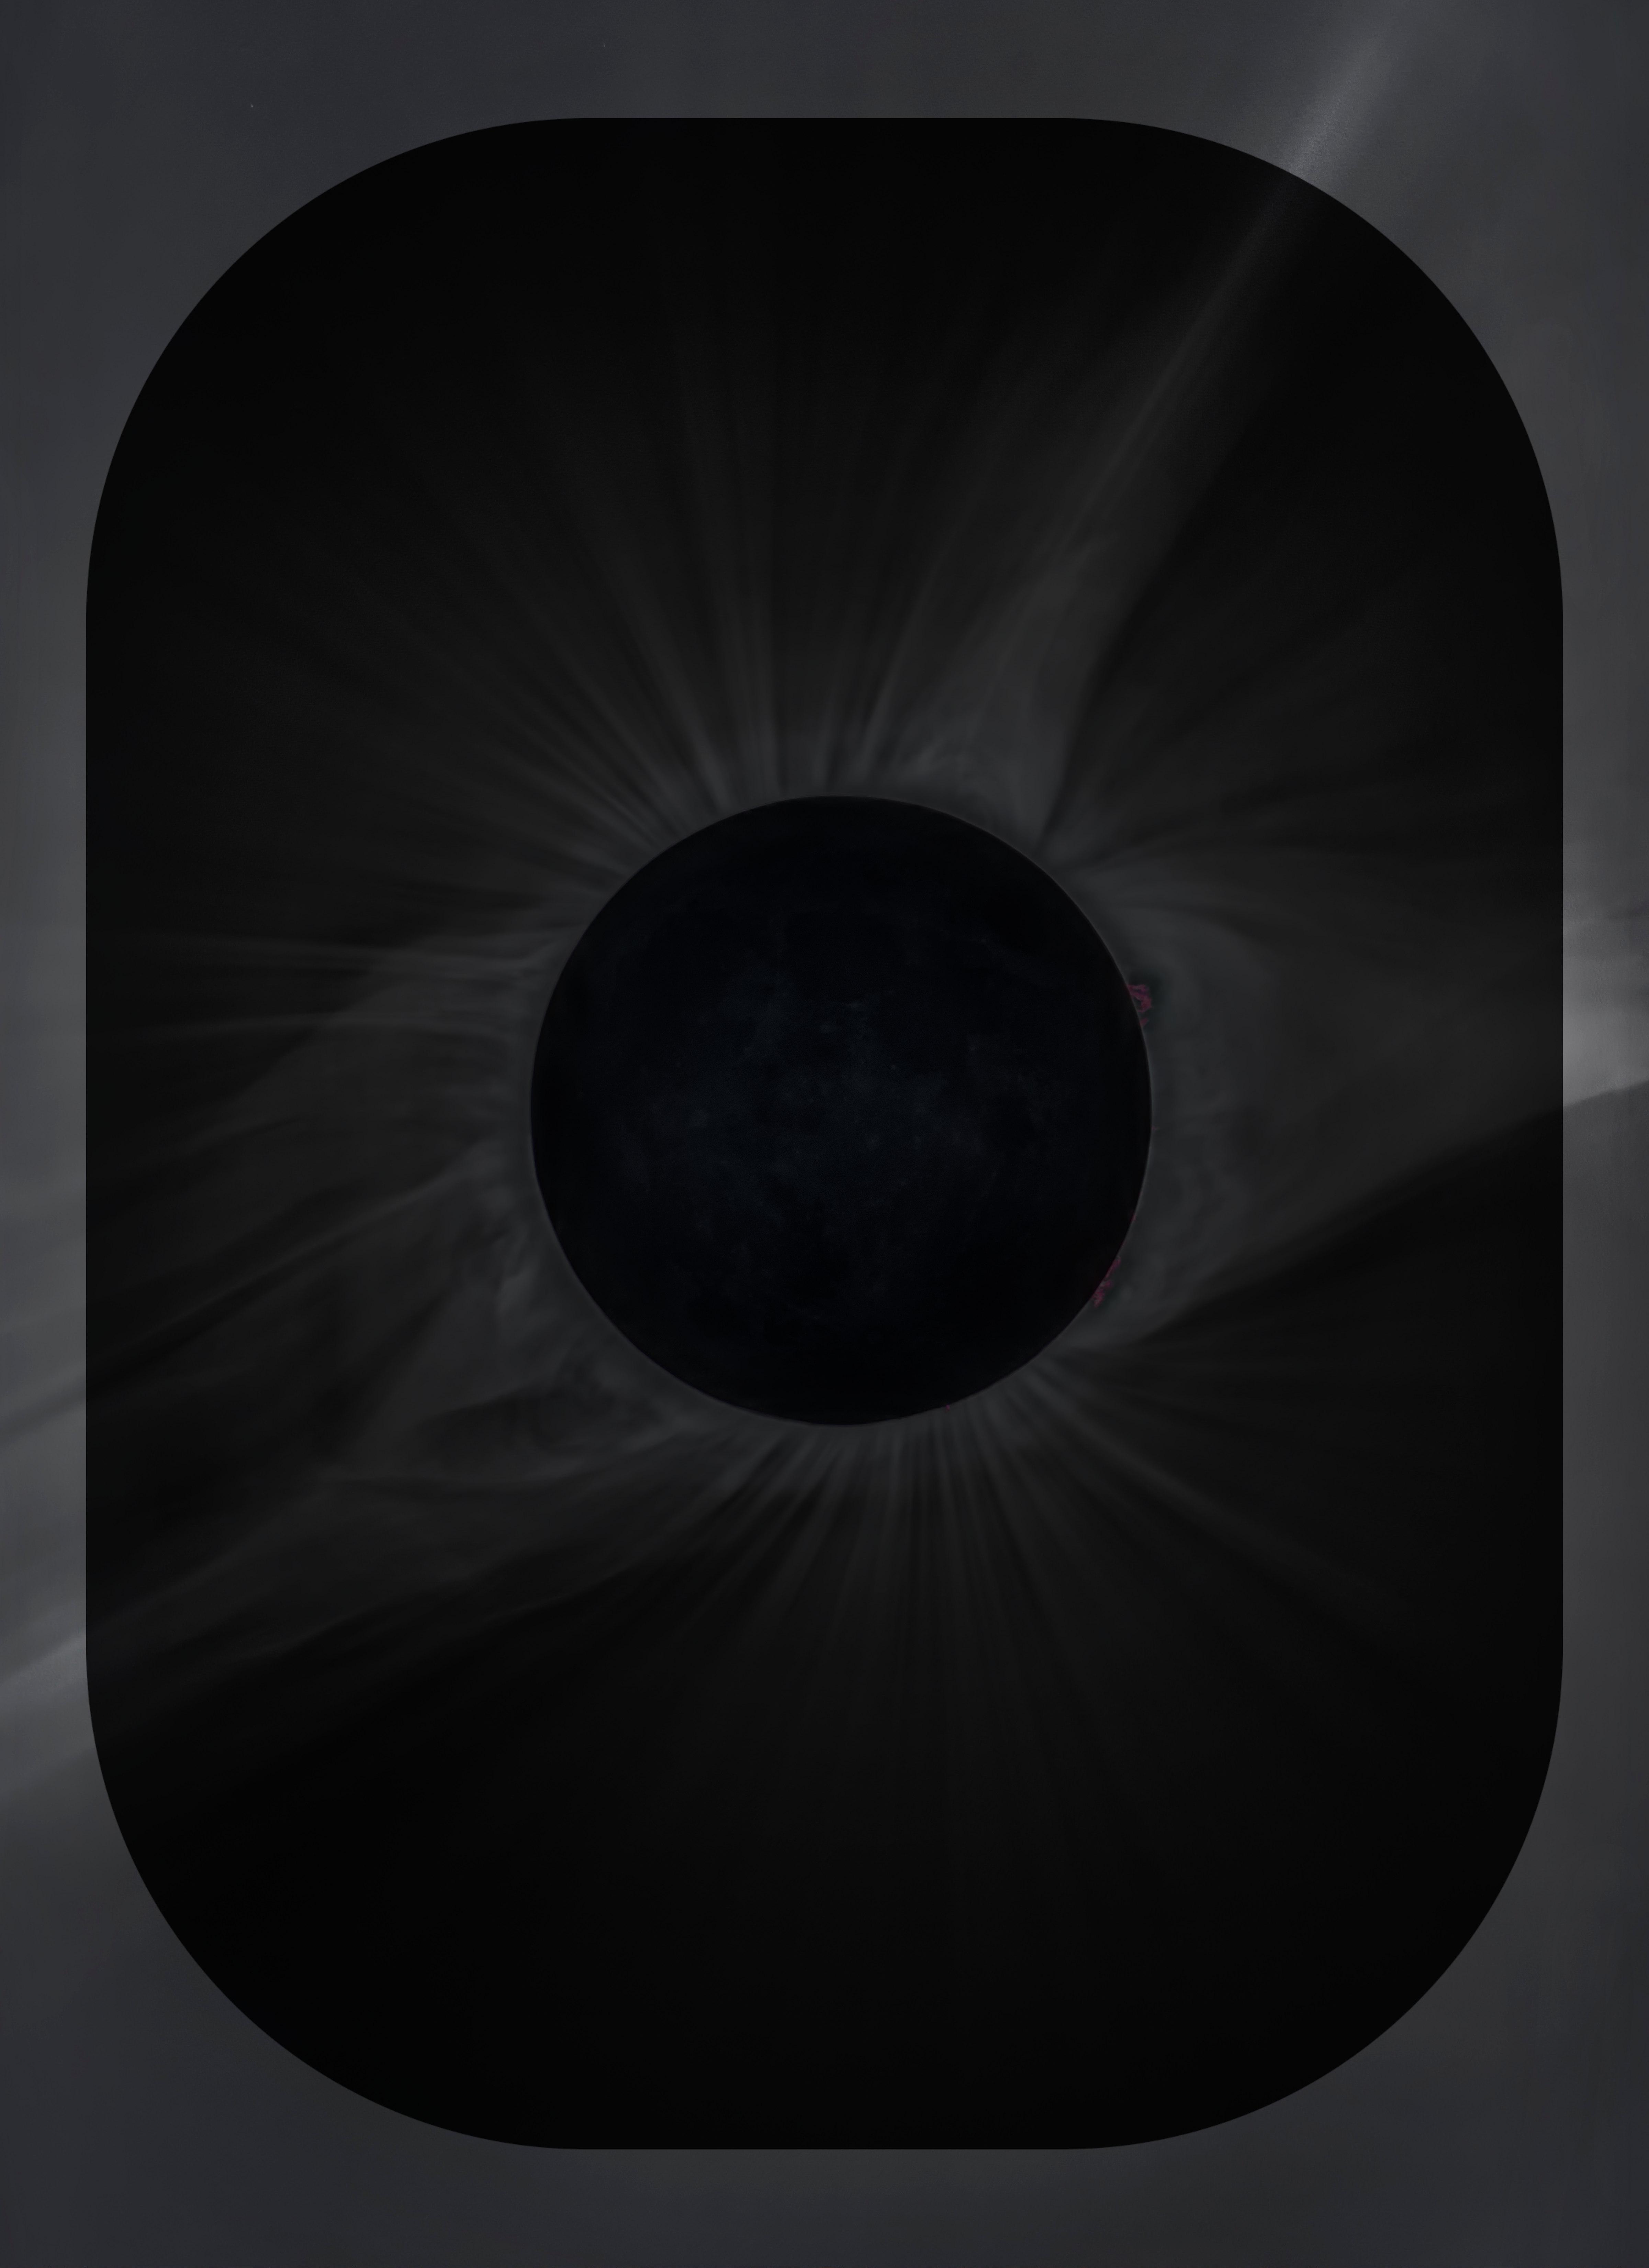
\includegraphics[width=\paperwidth,height=\paperheight]{solar-eclipse.jpeg}}

\renewcommand{\thefigure}{\color{Red}\Fontauri{\arabic{figure}}}
\renewcommand\thefootnote{\color{Red}\Fontauri{\arabic{footnote}}}

\let\oldfootnote\footnote
    \renewcommand{\footnote}[1]{\oldfootnote{\color{Red}\Fontauri\large#1}}
\begin{titlepage} % Suppresses headers and footers on the title page
	\centering % Centre everything on the title page
	\scshape % Use small caps for all text on the title page

	%------------------------------------------------
	%	Title
	%------------------------------------------------
	
	\rule{\textwidth}{1.6pt}\vspace*{-\baselineskip}\vspace*{2pt} % Thick horizontal rule
	\rule{\textwidth}{0.4pt} % Thin horizontal rule
	
	\vspace{0.75\baselineskip} % Whitespace above the title

        {\Huge Världarnas Utveckling \\} % Title
	
	\vspace{0.75\baselineskip} % Whitespace below the title
	
	\rule{\textwidth}{0.4pt}\vspace*{-\baselineskip}\vspace{3.2pt} % Thin horizontal rule
	\rule{\textwidth}{1.6pt} % Thick horizontal rule
	
	\vspace{1\baselineskip} % Whitespace after the title block
	
	%------------------------------------------------
	%	Subtitle
	%------------------------------------------------
	
	{Av \scshape\Large Svante Arrhenius \\} % Subtitle or further description
	
	\vspace*{1\baselineskip} % Whitespace under the subtitle
	
	%------------------------------------------------
	%	Editor(s)
	%------------------------------------------------

 	% Subtitle or further description

	\vspace{1\baselineskip} % Whitespace before the editors

        {\small Med 45 Illustrationer \\Fjärde Oförändrade Upplagan}

    %------------------------------------------------
	%	Cover photo
	%------------------------------------------------
	
	%\includegraphics[scale=1]{cover}
	
	%------------------------------------------------
	%	Publisher
	%------------------------------------------------

	\vspace*{\fill}% Whitespace under the publisher logo
	
	Stockholm 1906 % Publication year
	
	{\small Hugo Gebers Förlag} % Publisher

	\vspace{1\baselineskip} % Whitespace under the publisher logo

        Internet Archive Online Edition  % Publication year
	
	{\small Erkännande-IckeKommersiell-DelaLika 4.0 Internationell } % Publisher
\end{titlepage}
\setlength{\parskip}{1mm plus1mm minus1mm}
\clearpage
\pagestyle{fancy}
\fancyhf{}
\cfoot{\Fontauri{\thepage}}
\Large
\tableofcontents
\clearpage
\listoffigures
\clearpage
\section*{Företal till Första Upplagan.}
\paragraph{}
Då jag för omkring sex år sedan var sysselsatt med utarbetandet av min »Lehrbuch der kosmischen Physik,» kunde jag ej undgå att känna de stora svårigheter, som vidlådde förklaringen enligt dittills rådande åsikter av ett stort antal fenomen, särskildt dem som stodo i sammanhang med kosmogoniska spörsmål. Jag fann att det dittills försummade strålningstrycket med framgång kunde användas för förstående av en stor del av dessa förut svårtydda företeelser. Jag använde därför också denna förut förbisedda naturkraft i mycket vidsträckt grad vid behandlingen av nämnda företeelser i sagda lärobok.

Oaktadt de av mig försökta utredningarna vid deras första framträdande, såsom ju naturligt är, alls icke kunde göra anspråk på att bliva oförändrade i alla detaljer, mottogos de likväl av den vetenskapliga världen med ovanligt stort intresse och välvilja. Detta uppmuntrade mig att alltjämt söka efter förklaring över de mest framskjutna av de talrika gåtor som överallt möta på detta område. Jag har på detta sätt infogat några nya delar i det system av utläggningar angående världssystemens utveckling, som jag grundlagt först i en afhandling inlämnad till vetenskapsakademien i Stockholm 1900, strax därefter aftryckt i Physikalische Zeitschrift, och sedan vidare utbildat i Lehrbuch der kosmischen Physik.

Det säges ju, och icke utan berättigande, att vetenskapliga åsikter först böra debatteras inom fack-kretsar och där vinna erkännande, innan de framläggas inför en större publik. Det kan ej förnekas att största delen av de hugskott, som offentliggöras angående kosmogoniska frågor, aldrig skulle kommit i beröring med tryckpressen, om ofvannämnda betingelser iakttagits, ävensom att det arbete som blifvit nedlagdt på deras tryckning bättre kunnat användas. De sex år, som förflutit sedan mina första försök i denna riktning delgåfvos den vetenskapliga världen, och det välvilliga mottagande som desamma rönt, ävensom de rikliga tillfällen jag under denna tid haft att granska och förbättra mina utläggningar, anser jag vara mera än tillräckliga för att tillåta mig framlägga mina åsikter inför en större allmänhet.

I själfva verket har problemet angående världsutvecklingen alltid utgjort föremål för den tänkande allmänhetens synnerliga intresse. Och utan tvifvel kommer det att bibehålla den kanske främsta platsen bland alla frågor, som ej beröra direkt praktiska spörsmål. Den lösning, som hvarje tid gifvit detta älsklingsproblem, utgör en trogen bild av tidens tänkesätt på naturvetenskapligt område. I detta afseende har jag den lifliga förhoppning, att nedan gifna framställning skall till fullo motsvara den storartade utveckling, som fysiken och kemien nått vid sista sekelskiftet.

Före upptäckten av energiens oförstörbarhet omfattade de kosmogoniska spörsmålen endast frågan om, huru materien blifvit samlad på det sätt att de nu förefintliga himlakropparna däraf framgått. De främsta tankarna på detta område innehållas i Herschels åsikt om nebulosornas utveckling och Kant-Laplaces hypotes om solsystemens bildning ur världstöcken. Den förstnämnda åsikten synes alltmer bestyrkas av iakttagelsen. Däremot lider den Kant-Laplaceska hypotesen av så stora svårigheter, att man sett sig nödsakad att övergifva den, oaktadt den en lång tid ansetts såsom blomman av den kosmogoniska spekulationen. Att såsom Kant försöka bilda sig ett begrepp om, huru högeligen regelbundna sysystem av himlakroppar kunnat uppstå ur ett absolut oordnadt kaos är att sträfva efter lösningen av ett på grund av dess formulering fullkomligt olösligt problem. För öfrigt ligger det en motsägelse i alla försök att förklara världens uppkomst i dess helhet, såsom Stallo\footnote{Stallo: Concepts and theories of modern physics. 4 uppl. s. 276 London 1900.} med synnerlig styrka framhållit. »Den enda fråga, till hvilken en serie företeelser kan med rätta leda, angår dessa företeelsers beroende på och sammanhang med hvarandra.» I följd häraf har jag endast sökt visa, huru nebulosor kunna uppstå ur solar, och omvändt, hur solar uppstå ur nebulosor, och jag har antagit, att denna växelverkan ständigt pågått just såsom nu.

De kosmogoniska problemen försvårades i hög grad genom upptäckten av energiens oförstörbarhet. Mayers och Helmholtz' hypoteser om sättet för täckande av solens värmeförluster ha måst uppgifvas såsom otillräckliga och ha ersatts med en annan, grundad på de kemiska förhållandena i solens inre, belysta med den mekaniska värmeteoriens andra hufvudsats. En ännu större svårighet syntes resa sig därigenom att läran om energiens ständiga »försämring» leder till den slutsatsen, att världen allt mer närmar sig hvad Clausius kallar »värmedöden,» då all energi skall förefinnas jämnt fördelad i universum i form av rörelse hos kropparnas minsta smådelar. Även ur denna svårighet, som leder till ett för oss fullkomligt obegripligt slut på världsutvecklingen, har jag sökt en utväg, som går ut därpå, att energien »försämras» hos kroppar som befinna sig på sol-stadiet, däremot »förbättras» hos sådana, som tillhöra nebulosastadiet.

Slutligen har ännu en kosmogonisk fråga under den sista tiden blifvit mera aktuell än den förr var. Man trodde nämligen förr allmänt, att lif kan uppkomma ur oorganisk materia genom en process, kallad »själfalstring.»

Men liksom drömmen om själfalstring av energi --- »perpetuum mobile» --- numera fullkomligt fått vika för erfarenhetens negativa resultat i denna riktning, så är det sannolikt, att den stora erfarenhet, som häntyder på själfalstrings av lif orealiserbarhet, slutligen leder oss attantaga att den är alldeles omöjlig. För att förstå möjligheten av lifs uppträdande på planeterna, måste man då taga sin tillflykt till läran om Panspermien, hvilken jag gifvit en mot vetenskapens nuvarande utveckling svarande form genom att kombinera densamma med läran om strålningstrycket.

Det ledande motivet vid föreliggande bearbetning av de kosmogoniska spörsmålen har varit den åsikten, att världen på det hela taget ständigt varit likartad med hvad den nu är. Materien, energien och lifvet ha endast växlat form och plats i rymden.

En del av de slutsatser, till hvilka jag här kommit, har förut lämnats i populär form såsom föreläsningar i Kristiania 1903, i Göteborg, Stockholm och Norrköping 1906. Det sista kapitlet utgjorde föremål för en föreläsning i Frankfurt 1903 och i Stockholm vid högskolans 25-års-fest 1904 och har varit tryckt i »Nordisk tidskrift» 1905. Det första kapitlet, en föreläsning i Göteborg 1906, hållen till förmån för svenskar, som lidit förluster genom jordbäfningen i Kalifornien den 18 April 1906, har förut varit offentliggjordt i »Ord och bild» 1906.

Jag vill också begagna tillfället att tacka förläggaren av detta arbete Herr Hugo Geber för att han, i tillit till den svenska allmänhetens vakna intresse för de behandlade frågorna, möjliggjort denna boks utkommande även i svensk dräkt och med gedigen utstyrsel, förr än den lämnas till översättning på främmande tungomål.

Stockholm i Augusti 1906.

\begin{flushright}
\emph{Författaren.}
\end{flushright}
\clearpage
\section{Vulkaniska företeelser och jordbäfningar. Jordens inre.}
\paragraph{}
De svåra olyckor, som under den sista tiden (april 1906) träffat de blomstrande samhällena kring Vesuvius och i Kalifornien, ha åter riktat mänsklighetens uppmärksamhet på de våldsamma krafter, som uppenbara sig i form av vulkaniska utbrott och jordbäfningar.

De förluster av människolif, som registrerats i dessa två sista fall, äro likväl obetydliga i jämförelse med dem, som åtföljt åtskilliga äldre katastrofer av dylik art. Det häftigaste utbrott av vulkanisk art i nyare tid är otvifvelaktigt det av den 26-27 augusti 1883, hvarvid två tredjedelar av den 33 kvadratkilometer stora ön Krakatoa i den ostindiska Arkipelagen sprängdes i luften. Oaktadt denna ö var obebodd, dödades omkring 40,000 människor vid detta tillfälle, hufvudsakligen genom den flodvåg, som följde på utbrottet och förorsakade härjande översvämningar i de omgifvande trakterna. Ännu gräsligare var förstörelsen genom den kalabriska jordbäfningen, som bestod av flera jordskalf, under februari och mars månader 1783. Därvid förstördes den betydande staden Messina den 5 februari, och antalet av förlorade människolif genom dessa jordskalf uppskattades till omkring 100,000. Samma trakter, särskildt Kalabrien, hemsöktes för öfrigt, den 8 sept. 1905 av förödande jordskalf. En annan jordbäfning, som nämnes av historien på grund av den stora förlusten av människolif, ej mindre än omkring 90,000, var den som den 1 november 1755 härjade Portugals hufvudstad. Två tredjedelar av dessa människolif ödelades genom en fem meter hög flodvåg, som störtade in från hafvet.

Den bäst studerade av alla vulkaner är utan tvifvel Vesuvius. Under Roms blomstringstid var detta berg al helt fredlig art, en, så långt historien mindes, utslocknad vulkankägla. Kring detsamma hade på den utomordentligt bördiga jordmånen grekiska kolonier av en sådan rikedom uppblomstrat, att trakten kallades Stora Grekland (Græcia magna). Då inträffade år 79 efter Kristus det förödande utbrott, hvarigenom bland andra städer Herculanum och Pompeji ödelades. De våldsamt utbrytande gasmassor, som då strömmade ut ur jordens inre, ryckte bort en stor del av den gamla vulkankäglan, hvars återstod nu kallas Monte Somma, och de nedfallande stoftmassorna, blandade med utflytande lavaströmmar, byggde upp det nya Vesuvius. Detta har vid senare utbrott ofta betydligt ändrat sitt utseende och även i år fått en ny askkägla. Efter år 79 förekommo nya utbrott år 203, 472, 512, 685, 993, 1036, 1139, 1500, 1631 och 1660, alltså med ganska oregelbundna tidsintervall. Sedermera har Vesuvius varit i nästan oafbruten verksamhet, vanligen en alldeles ofarlig sådan, då endast rökmolnet över kratern angifvit, att den inre glöden alltjämt fortfarit (fig. 1). Mycket häftiga utbrott förekommo under denna tid år 1794, 1822, 1872 och 1906.

\begin{figure}[H]
\centering
\includegraphics[width=0.9\textwidth,keepaspectratio]{red/fig-01.png}
\caption{\Fontauri{Fig. 1. --- Vesuvius, sedd från ön Nisita under måttlig vulkanisk verksamhet.}}
\end{figure}
\paragraph{}
Helt annorlunda än dessa häftigt verksamma vulkaner förhålla sig andra, som knappast förorsaka nämnvärd skada. En sådan är vulkanen Stromboli mellan Sicilien och Kalabrien. Denna är sedan årtusenden i ständig verksamhet, dess utbrott följa hvarandra med tidsmellanrum uppgående till mellan mindre än en minut och tjugo minuter. Dess eld tjänar som ett slags naturlig fyrbåk för de sjöfarande. Naturligtvis är även denna vulkans kraft olika vid olika tider, för närvarande säges den vara i ovanligt häftig verksamhet. Mycket lugnt aflöpa också utbrotten av de stora vulkanerna på Hawai.

Den viktigaste beståndsdelen bland de kroppar, som stötas ut ur vulkanerna, är vattenånga. Därför utgör molnet över vulkankratern det säkraste kännemärket på vulkanens verksamhet. Vid de häftiga utbrotten stötas dessa ångmassor högt upp i luften, såsom av närstående bilder synes, bortåt åtta kilometer. Vesuvius själf är Fig. 2. Vesuvii utbrott år 1794; efter en samtida handteckning. 1300 m. högt över hafsytan, och med ledning däraf kan man uppskatta molnets höjd. Omstående bild återger en teckning av Poulett Scrope,som föreställer Vesuvii utbrott år 1822. I detta fall synes vindstilla råda.

\begin{figure}[H]
\centering
\includegraphics[width=0.45\textwidth,keepaspectratio]{red/fig-02.png}
\caption{\Fontauri{Fig. 2. --- Vesuvii utbrott år 1794; efter en samtida handteckning.}}
\end{figure}
\paragraph{}
Ångmassorna bilda då moln av en regelbunden form påminnande om utseendet av en pinie. Molnet över Vesuvius vid dess utbrott år 79 beskrifves av Plinius såsom hafvande ägt detta utseende. Då luften ej är så stilla, antager molnet en mera oregelbunden form (fig. 4). Moln, som stiga upp till så stora höjder som de nämnda, utmärka sig genom häftiga elektriska laddningar. De kraftiga blixtarna, som på grund häraf skjuta ut ur det svarta molnet, bidraga mycket till att öka intrycket av det hemska skådespelet.

\begin{figure}[H]
\centering
\includegraphics[width=0.75\textwidth,keepaspectratio]{red/fig-03.png}
\caption{\Fontauri{Fig. 3. --- Vesuvii utbrott år 1822 efter en samtida handteckning.}}
\end{figure}
\paragraph{}
Regnet, som störtar ned ur detta moln, blandas ofta med aska och ser då ut som bläck. Askan, som har en mellan ljusgrått, gulgrått och brunt till nästan svart växlande färg, är endast ytterst små droppar av lava, som kastats ut av de utströmmande gaserna och hastigt stelnat i luften. Större lavadroppar stelna till vulkanisk sand eller så kallade lapilli (d. v. s. stenar) och »bomber» hvilka ofta äro fårade och päronformade på grund av luftens motstånd. Dessa fasta produkter åstadkomma vanligen de största skadorna vid vulkaniska utbrott. Tyngden av de nedfallande massorna tryckte in taken på husen 1906. Ett 7 meter tjockt lager av aska inbäddade Pompeji i det skyddande täcke, som höljt detsamma till utgräfningarna i våra dagar. Därvid smög sig den fina askan och det regnblandade slammet tätt såsom en gipsform till de döda kroppar, som inhöljdes däri; de hårdnade sedermera såsom ett slags cement, och då sönderdelningsprodukterna av de döda kropparna spolats bort, kunde man med hjälp av cementformen erhålla de naturtrognaste afgjutningar av de förut däri inbäddade föremålen. På samma sätt bildas, där askan faller ned i hafvet, ett lager av vulkanisk tuff, i hvilken sjödjur och hafsalger inbäddas: av denna art är jorden i landskapet Campagna Felice vid Neapel. Större stenar genomdragna av otaliga gasblåsor, flyta kring på hafvet såsom pimpsten, de täras småningom sönder av hafsvågen till vulkanisk sand. Den kringdrifvande pimpstenen är stundom farlig eller hinderlig för skeppsfarten på grund av sin stora massa. Detta var exempelvis fallet vid Krakatoas utbrott 1883.

\begin{figure}[H]
\centering
\includegraphics[width=0.9\textwidth,keepaspectratio]{red/fig-04.png}
\caption{\Fontauri{Fig. 4. --- Vesuvii utbrott år 1872 enligt fotografi.}}
\end{figure}
\paragraph{}
Utom vattenångan utstötas även andra gaser, i främsta rummet kolsyra, men även ångor av svafvel, svafvelväte, klorväte och salmiak samt mera sällan klorider av järn och koppar, borsyra med mera. En stor del av dessa kroppar utfälles rätt hastigt på vulkanväggarna vid vulkangasernas hastiga afkylning; en annan del av mera flyktiga beståndsdelar, såsom kolsyra, svafvelväte och klorväte, kan breda ut sig på större sträckningar och förgöra genom sin hetta och giftighet alla människo- och djurlif, som komma i gasströmmens väg. Detta var nu fallet vid den sorgliga förödelsen av St. Pierre, då 30,000 människolif spilldes genom Mont Pélées utbrott d. 8 maj år 1902. Även Plinius d. ä. dödades vid Vesuvii utbrott år 79 av kväfvande gaser. Man har i kratern Kilauea iakttagit utströmning av vätgas, hvilken emellertid vid utträdet ur lavan i luften förbränts till vatten.

Vulkanaskan kan stundom av luftströmmarna föras bort över stora sträckor, så från Sydamerikas västkust till Antillerna, från Island till Norge och Sverige, från Vesuvius (1906) till Holstein. Mest bekant i detta afseende är Krakatoas utbrott, hvarvid den fina askan slungades ända till 30 kilometers höjd och de finaste partiklarna småningom spriddes av vindarna till alla delar av jorden, där de under de närmaste två åren förorsakade de praktfulla soluppgångar eller solnedgångar, som fått namn av »röda skenet.» Även efter Mont Pélées utbrott iakttog man i Europa det röda skenet. Stoftet från Krakatoa gaf också material till de 1883-1892 iakttagna så kallade »lysande nattmolnen,» som under den sista tiden sväfvade på omkring 80 kilometers höjd och därför voro solbelysta långt efter solens nedgång.

\begin{figure}[H]
\centering
\includegraphics[width=0.8\textwidth,keepaspectratio]{red/fig-05.png}
\caption{\Fontauri{Fig. 5. --- Vesuvii utbrott år 1906 enl. fotografi; hufvudsakligen askmoln.}}
\end{figure}
\paragraph{}
Ett synnerligt stort intresse har kratern Kilauea på den höga vulkanen Mauna-Loa på Hawai --- denna vulkan är ungefär så hög som Mont Blanc --- ådragit sig. Denna krater bildar en stor lavasjö av omkring 12 kvadratkilometers utsträckning --- den växlar emellertid betydligt med tiden. Den kokande, rödheta lavamassan afger under lätta explosioner ständigt gasmassor, hvarvid eldfontäner av omkring 20 meters höjd spruta upp i luften. Stundom utgjuter sig lavasjön genom sprickor i kraterns kant och flyter ut i form av en lavaström längs efter bergets sida, intill dess lavasjöns yta sjunkit under sprickorna. Denna lava är vanligen at jämförelsevis lättflytande beskaffenhet och breder därför ut sig tämligen jämnt över stora ytor. Av liknande art äro de lavaflöden, som stundom gjutits över tusentals kvadratkilometer på Island --- särskildt storartadt var det så kallade Laki-utbrottet år 1783, som, oaktadt det ägde rum i obygden, likväl förorsakade ganska stor skada. I äldre geologiska perioder, särskildt den tertiära, ha oerhördt stora lavatäcken av sådan art gjutit sig ut exempelvis över England och Skottland (över 100,000 kv. km.), över Dekkan i Indien (400,000 kv. km., till en höjd av stundom 2,000 m.) och över Wyoming, Yellowstone Park, Nevada, Utah, Oregon och andra delar av Nordamerikas Förenta stater samt British Columbia.

I andra fall innehåller den långsamt framflytande lavan massor av gaser, som vid lavans stelnande gå bort och spränga sönder densamma i skrofliga block, då den bildar så kallad blocklava (fig. 6). Även lavaströmmarna åstadkomma ofantlig förödelse, då de tränga ned till odlade trakter, men på grund av sin långsamma rörelse förorsaka de endast ringa förlust av människolif.

Då den vulkaniska verksamheten småningom minskas och upphör, stanna vanligen spår av densamma kvar uti de utströmningar av varmt vatten och gaser, som på många trakter observeras, där under tertiärtiden mäktiga vulkaner utstötte sina lavaströmmar. Hit höra de berömda gejsrarna på Island, i Yellowstone Park och på Nya Zeeland, de i medicinskt afseende högt skattade varma källorna i Böhmen (t. ex. Karlsbadersprudeln), de vattenånga utkastande fumarolerna i Italien, Grekland och andra länder, mofetterna med deras kolsyre-utströmningar --- sådana förekomma ymnigt i det så kallade Eifel-området nära Rhen, i hundgrottan vid Neapel och i dödsdalen på Java --- solfatarerna, som afgifva svafvelångor, vätesvafla och svavelsyrlighet --- sådana finnas vid Neapel på de phlegreiska fälten och i Grekland ---, samt en del av de så kallade slamvulkanerna, hvilka stöta ut slam, saltvatten och gaser, vanligen kolsyra och kolväten, till exempel de vid Parma och Modena i Italien samt vid Kronstadt i Siebenburgen befintliga.

\begin{figure}[H]
\centering
\includegraphics[width=0.9\textwidth,keepaspectratio]{red/fig-06.png}
\caption{\Fontauri{Fig. 6. --- Blocklava å Mauna Loa.}}
\end{figure}
\paragraph{}
De slocknade vulkanerna, bland hvilka några höra till jordens högsta berg, såsom Aconcagua i Syd-Amerika (6,970 m.) och Kilimandjaro i Afrika (6,010 m.), lida ofta en snabb förstöring genom regnets inflytande, emedan de till stor del äro uppbyggda av löst material, vulkanisk aska, mellanlagrad med lavaströmmar. Dessa, som ha en radial utsträckning, skydda underliggande delar från att föras bort av vatten, och man får på detta sätt vid lavaströmmarnas kanter formliga skärningar genom den gamla vulkanen och även nedanför liggande sedimentära jordaflagringar. Ett intressant exempel på sådant förhållande visar den gamla vulkanen Monte Venda vid Padua. Man kan där iakttaga, huru den varma lavan, där den utgjutit sig över sedimentära kalkstenar, förvandlat dessa till marmor till ett djup av omkring 1 meter. Stundom äro även kalkstenar, liggande över de gamla lavatäckena, på detta sätt omvandlade, hvilket visar, att lavan ej blott flödat över kraterns rand utan även från sidan trängt in i springor mellan två olika skikt i kalkstenen. Sådana massformade underjordiska utgjutningar förekomma i de så kallade lakkoliterna i Utah. I dessa ha de överliggande lagren pressats upp av den påträngande lavamassan, som emellertid har stelnat innan den hunnit upp till jordytan och kommit att bilda en vulkan. Av likartadt ursprung äro en hel del graniter, s. k. batholiter, hvilka ymnigt förekomma i Norge, Java, Skottland o. s. v. Stundom står endast en kärna av stelnad lava kvar av hela det eldsprutande berget. Dessa kärnor, som ursprungligen fyllt kraterröret, äro mycket vanliga i Skottland och Norra Amerika, där de kallas »Necks.» I Coloradoplatån ha flera floder nedskurit så kallade Canons med nästan vertikala väggar. En teckning av Dutton visar en sådan över 800 m. hög vägg, i hvilken fyra lavafyllda sprickor trängt upp till ytan (fig. 8). Öfver den ena finnes ännu en liten vulkanisk askkägla, medan de, som sannolikt afslutat de tre andra springorna, äro bortspolade, så att gångarna sluta med små »necks.» Tydligen har lättsmält lava --- den som innehåller mycket magnesia och järnoxid är mera lättflytande än den som innehåller mycket kiselsyra, fluiditeten ökas för öfrigt genom närvaro av vatten --- plötsligen trängt in i de förut befintliga sprickorna och nått ända fram till jordytan, innan den stelnat. Man måste antaga, att den drifvande kraften har varit ganska betydande för att den nödvändiga utströmningshastigheten skall ha blifvit uppnådd.

\begin{figure}[H]
\centering
\includegraphics[width=0.9\textwidth,keepaspectratio]{red/fig-07.png}
\caption{\Fontauri{Fig. 7. --- Mato Tepee i Wyoming, U. S. A. En typisk vulkanisk »neck.»}}
\end{figure}
\paragraph{}
Då Krakatoa år 1883 sprängdes i luften, stannade hälften av dess vulkan kvar på platsen. Denna visar mycket tydligt genomskärningen av en askkägla, som ännu lidit mycket ringa inverkan av vattnets förstörelsearbete. Man ser här i midten den ljusa lavaproppen i vulkanröret, och från denna utgå ljusare lavabäddar, mellan hvilka mörkare asklager synas.

För öfrigt har man iakttagit en påfallande regelbundenhet i afseende på vulkanernas fördelning på jordytan. Nästan alla vulkaner ligga i närheten av hafvet, några vulkaner finnas visserligen i Ost-Afrika, men de ligga i stället nära de stora sjöarna vid ekvatorn. Några vulkaner, som angifvits såsom belägna i Centralasien, äro tvifvelaktiga. Emellertid saknas vulkaner vid många hafskusten såsom vid Australiens kust och vid Norra Ishafvets långa kustlinjer norr om Asien, Europa och Amerika: Endast där stora sprickor i jordskorpan förefinnas längs hafskusterna, förekomma vulkaner. Där dylika sprickor i skorpan förekomma, men haf (eller mycket stora insjöar) ej finnas i närheten, exempelvis i Österrikes alptrakter, förekomma ej heller vulkaner, dessa trakter äro däremot kända för sina jordbäfningar.

\begin{figure}[H]
\centering
\includegraphics[width=0.9\textwidth,keepaspectratio]{red/fig-08.png}
\caption{\Fontauri{Fig. 8. --- Lavafyllda sprickor med en vulkanisk askkägla på Torowheap-canon, Coloradoplatån. Skematisk bild.}}
\end{figure}
\paragraph{}
Redan tidigt har den föreställningen gjort sig gällande, att jordens smälta inre massa genom vulkanerna tränger fram till jordytan. Man har försökt att uppskatta djupet av vulkanhärdarna och kommit till ganska olikartade resultat. Så t. ex. har man för vulkanhärden under den vulkan, Monte Nuovo, som år 1538 uppkastades på de phlegreiska fälten vid Neapel, beräknat ett djup av mellan 1,3 och 60 kilometer, för Krakatoa har man funnit mer än 50 kilometer, o. s. v. Alla dessa beräkningar synas tämligen betydelselösa, då vulkanerna sannolikt ligga över veck på jordskorpan, i hvilka den flytande massan (magman) i jordens inre kilformigt tränger in, så att man troligen har svårt att ange hvar magmahärden slutar och vulkanröret börjar. Vid Kilauea har man ovillkorligen det intrycket, att man står framför en öppning i jordskorpan, genom hvilken jordens smälta massa direkt träder i dagen (fig. 9).

Angående jordskorpan vet man genom iakttagelser i borrhål i skilda världsdelar, att temperaturen mot djupet stiger ganska hastigt --- i medeltal med ungefär 30 grader för hvarje kilometer; de djupaste borrhål äro för öfrigt ej fullt 2 kilometer djupa (Paruchowitz i Schlesien 1,96, Schladebach vid Merseburg 1,72 km.). Stiger nu temperaturen med 30C pr kilometer, så måste på ett djup av 40 kilometer en temperatur vara uppnådd, vid hvilken alla vanligare bergarter skulle smälta. Nu stiger visserligen smältpunkten med trycket, men betydelsen av denna omständighet har förr mycket överdrifvits, då man trodde att möjligen på denna grund jordens inre skulle kunna vara fast. Såsom Tammann visat genom direkta försök, är det sannolikt, att smälttemperaturen stiger endast till ett visst tryck, för att sedermera, vid ytterligare stegring av trycket, åter sjunka. Det nyss beräknade värdet kommer därför att något höjas, men om man antager, att andra bergarter förhålla sig såsom diabas enligt Barus, d. v. s. att deras smältpunkt stiger 1° C. för 40 atmosfärers tryck, motsv. 155 m. djup, så finner man, att den fasta jordskorpan ej har större tjocklek än mellan 50 och 60 kilometer. På större djup vidtager således den smälta massan. På grund av kiselsyrans större lätthet kommer denna att koncentreras i smältans högre skikt, medan de mera järnoxidhaltiga, de s. k. basiska, delarna av magman på grund av sin tyngd företrädesvis samla sig i dess djupare delar. Denna magma hafva vi att föreställa oss såsom en ytterst trögflytande vätska, liknande asfalt. Genom Days och Alléns undersökningar har det visat sig, att i ändarna stödda stafvar (30 x 2 x 1 m. m.) av åtskilliga mineral, sådana som fältspaterna mikroklin och albit, kunnat bibehålla sin form under tre timmar, utan att märkbart böjas, oaktadt deras temperatur legat omkring 100° C. över smältpunkten och de vid uttagningen ur ugnen varit fullkomligt smälta eller rättare förglasade. Dessa silikat förhålla sig helt annorlunda än de substanser, med hvilka vi äro vana att arbeta, såsom vatten och kvicksilfver.

\begin{figure}[H]
\centering
\includegraphics[width=0.9\textwidth,keepaspectratio]{red/fig-09.png}
\caption{\Fontauri{Fig. 9. --- Kilaueas krater, Hawaï.}}
\end{figure}
\paragraph{}
Den omrörning och diffusion, som förekommer i magman, särskildt dess mycket trögflytande, ofvantill belägna, sura, partier, är således ytterst ringa, så att magman, likasom albiten vid Days och Alléns försök, skenbart förhåller sig såsom en fast kropp. Magman under nära hvarandra belägna vulkaner såsom Etna, Vesuvius och Pantellaria kan därför, såsom erfarenheten angående deras lava visar, ha ganska olika sammansättning, utan att man därför med Stübel behöver antaga, att dessa tre vulkanhärdar äro fullkomligt isolerade från hvarandra.

Lavan i Vesuvius har befunnits äga en temperatur av 1000 à 1100° C. vid lavaströmmens nedre ände. Ur förekomsten i lavan av vissa kristaller, såsom av leucit och olivin, hvilka man av vissa skäl antar ha bildats före lavans utträde ur kratern, sluter man till, att dennas temperatur, innan den lämnade vulkanröret, ej kan hafva varit högre än omkring 1400° C.

Det vore emellertid orätt att ur lavans i Vesuvius temperatur draga den slutsatsen, att vulkanhärden ligger på ett djup av inemot 50 kilometer. Dess djup är sannolikt mycket mindre, kanske ej ens 10 kilometer, emedan här, liksom överallt där vulkaner förekomma, jordskorpan är starkt veckad, så att magman på vissa ställen, där just vulkanerna böra förekomma, kommer mycket närmare jordytan än under normala förhållanden.

Vattnets betydelse för vulkanernas bildning beror sannolikt därpå, att detsamma i närheten av sprickor under hafsbottnen tränger ned mot djupet. Då det når ett skikt, hvars temperatur är 365° (vattnets s. k. kritiska temperatur), kan det ej längre förefinnas i flytande tillstånd. Detta hindrar emellertid ej, att det tränger vidare ned i djupet, fastän förgasadt. Då det når magman, absorberas det av denna i hög grad. Detta beror därpå, att vatten vid temperaturer av över 300 grader är en starkare syra än kiselsyra, som därför av vattnet uttränges ur dess föreningar, silikaten, som utgöra huvudbeståndsdelen av magman. Ju högre temperaturen är, desto större blir magmans förmåga att uppsupa vatten. Genom detta upptagande av vatten sväller magman och blir samtidigt mera lättflytande. Magman pressas därför ut under utöfvande av ett tryck, som fullkomligt motsvarar det osmotiska trycket vid inträngande av vatten i en lösning, exempelvis av socker eller salt. Detta tryck kan bliva så starkt, att det uppgår till tusentals atmosfärer. Av detta tryck kan magman lyftas upp genom vulkanrören, även om dessas höjd skulle stiga till bortåt 6000 meter över hafvet. Då magman nu stiger upp i vulkanröret, afkyles den småningom, dess förmåga att hålla vatten absorberadt minskas med temperaturen. Vattnet bortgår därför under häftiga kokningsfenomen och rycker med sig droppar eller större massor av lava, som faller ned såsom aska och pimpsten. Även sedan lavan flutit ut ur kratern, afkyles den långsamt och afger allt mera vatten, som söndersliter detsamma under bildande av blocklava. Står däremot lavan jämförelsevis stilla i vulkankratern, såsom i Kilauea, afgår vattnet långsammare, och till följd av de översta lavalagrens långa beröring med luften hålla de jämförelsevis litet vatten --- detta är så att säga utluftadt ---, och deras lavaströmmar bilda därför vid stelnandet mera jämna ytor.

I åtskilliga fall har man (Stübel och Branco) påvisat vulkaner, som äro oberoende av brottsprickor i jordskorpan. Detta är exempelvis fallet med några vulkaner från äldre (tertiära) tider i Schwaben. Man kan väl tänka sig, att trycket på grund av magmans svällning blir så stort, att det förmår genombryta jordskorpan, där denna är tunn, även om ingen spricka där förut förefinnes.

Fortsätta vi nu undersökningen av magman på större djup, så finnes ingen anledning att antaga, att ej temperaturen fortfarande stiger mot jordens inre. På ett djup av 300 a 400 kilometer bör temperaturen slutligen bli så hög (omkring 10,000° C.), att intet ämne där förmår att bestå annat än i gasform. Innanför detta skikt bör således jordens inre vara gasformigt. På grund av våra undersökningar angående gasernas förhållande vid höga temperaturer och tryck ledas vi att antaga, att gaserna i jordens innersta förhålla sig ungefär såsom en ytterst trögflytande magma; i vissa afseenden kunna de snarast jämföras med fasta kroppar. Särskildt är deras sammantryck-barhet ytterst ringa. Man skulle kunna tro, att det vore nära nog omöjligt att få någon som helst kunskap om dessa lagers förhållande; genom jordbäfningarna få vi emellertid någon kännedom därom. Dessa lager utgöra den ojämförligt största delen av jordmassan och måste ha en betydande specifik vikt, då jordens specifika vikt i medeltal är 5,52 och de yttre lagren, såsom världshafvet och de av oss kända jordmassorna, ha lägre specifik vikt (de vanliga bergarterna ha specifika vikter mellan 2,5 och 3). Man har därför antagit, att jordens innersta delar äro metalliska, särskildt har Wiechert förfäktat denna åsikt. Sannolikt utgör järn hufvudmassan i denna jordgas. Därför talar den omständigheten, att järn, såsom Spektralanalysen lär oss, utgör en synnerligen viktig beståndsdel av solen, att vidare järn utgör hufvudmassan av de metallrika delarna i meteoriter, och slutligen tyder jordmagnetismen därpå, att järn i stora mängder förefinnes i jordens inre. Man har också anledning att tro de i naturen förekommande järnen, t. ex. det bekanta järnet från Ovifak i Grönland, vara av vulkaniskt ursprung. De i jordens gasformiga inre förekommande ämnena förhålla sig på grund av sin täthet i kemiskt och fysikaliskt afseende ungefär såsom vätskor. Då metaller sådana som järn säkerligen även vid mycket höga temperaturer hafva vida högre specifik vikt än deras oxider och dessa högre än deras silikat, så måste vi antaga att gaserna i jordens allra innersta nästan uteslutande bestå av metaller, de yttre delarna däremot hufvudsakligen innehålla oxider och de yttersta mest silikat.

Beträffande den längst ut liggande smälta magman är det sannolikt, att den ofta, då den tränger in i högre lager i form av batholiter, till följd av afkylningen delas i två delar, hvaraf den ena är lättare och gasformig och innehåller vatten och däri lösliga beståndsdelar, medan den andra, den tyngre, till sin hufvudmassa består av silikat med ringa halt av vatten. Den lättrörliga, vattenrika delen afsöndrar sig i de högre skikten, och tränger in i kringliggande sedimentära lager, särskildt i deras sprickor, och fyller dem med stora kristaller, ofta av metallurgiskt värde, såsom tenn-, koppar- och andra malmer, medan vattnet sakta dunstar bort genom de ofvanliggande delarna. Den trögflytande silikatmassan stelnar däremot, till följd av sin ringa fluiditet, till glas eller, om afkylningen sker långsamt, i små kristaller.

Vi återgå nu till jordbäfningarna. Intet land är fullkomligt förskönadt för jordbäfningar. I vårt land och grannländerna, särskildt norra Ryssland, förekomma de emellertid endast i mycket ofarliga former. Detta beror därpå, att jordskorpan här legat orubbad genom långa geologiska tidrymder och ej bräckts sönder i några sprickor. Den jämförelsevis starka jordbäfning, som den 23 okt. 1904 skakade vårt land, särskildt dess västkust, i ovanligt häftig grad, dock utan att orsaka nämnvärd skada, några skorstenar skakades ned, härrörde från en for våra nordiska förhållanden jämförelsevis betydande skrynkla i jordskorpan ute i Skagerack, en fortsättning av det djupaste vecket på Nordsjöns botten, den så kallade norska rännan, som går fram utanför Norges kust. Även andra starkare jordskalf, som observerats i vårt land, t. ex. de av den 22 dec. 1759 och den 13 april 1851 synas ha utgått från samma trakt, I Europa träffas Italien och Balkanhalfön samt de österrikiska så kallade karstländerna jämförelsevis ofta av jordskalf.

Enligt en av British Association tillsatt kommitté för undersökning av jordbäfningar, hvilken mycket väsentligt bidragit till kännedomen av dessa viktiga naturfenomen, härröra de som äro av någon betydelse från bestämda centra, som äro angifna på vidstående karta (fig. 10). Av dessa äro de viktigaste det, som omfattar bortre Indien, Sundaöarna, Nya Guinea och Norra Australien, på kartan betecknadt med F. Från detta område ha under sexårsperioden 1899-1904 utgått ej mindre än 249 jordskalf, som iakttagits på långt aflägsna observationsorter. Det nämnda jordbäfningscentret hänger nära tillsammans med det japanska med E betecknade, som gifvit upphof till 189 jordskalf. Därnäst kommer det vidsträckta distriktet K, omfattande de viktigaste veckningarna i den gamla världens jordskorpa med bergskedjor från Alperna till Himalaya, med 174 jordbäfningar. Detta distrikt är intressant, emedan det företer en stor mängd jordbäfningar, oaktadt det nästan helt och hållet ligger på landområde. Närmast efter detta komma områdena A, B och C med 125, 98 och 95 jordskalf. De ligga vid de stora brottytorna i jordskorpan längs Amerikas Stilla Hafskust och i Karaibiska hafvet. Detsamma gäller om distriktet D med 68 jordskalf. De tre sistnämnda B, C och D, likasom distriktet G mellan Madagaskar och Indien med 85 jordskalf, överträffas likväl skenbart av distriktet H i östra Atlanten med dess 107 jordskalf. Dessa sistnämnda äro nämligen jämförelsevis svaga, och deras noggranna upptecknande beror sannolikt på, att en stor mängd jordbäfningsobservatorier ligga i detta distrikts närmaste omgifning. Detsamma är fallet med de mycket få jordskalfven från distrikten I utanför New Foundland och J mellan Island och Spetsbergen med resp. 31 och 19 jordskalf. Sist på listan kommer distriktet L kring sydpolen med 8 jordskalf. Detta ringa antal är nog beroende på bristen på observationsorter i dessa trakter. Till dessa har slutligen kommit ett nytt distrikt M, som sträcker sig åt SSW från Nya Zeeland. Från detta distrikt härstamma ej mindre än 75 starka jordskalf, som registrerats av Discoveryexpeditionen (70° S. Br., 178 Ö. L.) under tiden 14 Mars till 23 Nov. 1903.

\begin{figure}[H]
\centering
\includegraphics[width=0.9\textwidth,keepaspectratio]{red/fig-10.png}
\caption{\Fontauri{Fig. 10. --- Karta utvisande läget av de viktigaste jordbäfnings centra enligt British Associations undersökning.}}
\end{figure}
\paragraph{}
Jordbäfningarna förekomma vanligen i så kallade svärmar. Så räknade man i Mars 1868 mer än 2000 jordstötar på Hawai. Vid de jordskalf, som 1870-73 härjade landskapet Phokis i Grekland, iakttogos stundom jordstötar, som följde på hvarandra med mellantider av tre sekunder, under långa tider. Under jordbäfningstiden, som omfattade $3\frac{1}{2}$ år, beräknas omkring en half million jordstötar och en fjärdedels million underjordiska dån, som ej åtföljdes av märkliga jordskalf, ha inträffat. Bland dessa jordskalf voro likväl endast omkring 300 åtföljda av nämnvärd förstörelse och blott 35 ansågos värda omnämnande i tidningarna. Även jordstöten av den 23 oktober 1904 tillhörde en svärm, som varade från den 10 till den 28 oktober, då talrika småstötar, särskildt den 24 och 25 oktober gjorde sig kända. Jordbäfningen i San Francisco började den 18 april 1906 kl. 5 t. 12 m. 6 s. förmiddagen (pacific tid.) och var slut kl. 5 t. 13 m. 11 s. f. m., motsvarande en varaktighet av en minut och fem sekunder. Inom en timme därefter iakttogos tolf mindre stötar. Före kl. 6.52 e. m. hade ytterligare nitton jordskalf annoterats, och dylika mindre stötar återkommo under flera dygn efteråt.

Till följd av detta förekomstsätt inträffa vanligen svagare stötar före de häftiga, förstörande, och tjänstgöra sålunda såsom ett slags varningstecken. Men ganska ofta är detta dessvärre icke fallet, så t. ex. vid de jordbäfningar, som förstörde Lissabon 1755 och Caracas 1812 och de som anställde ovanligt stora härjningar i Agram 1880 och nu senast i San Francisco 1906. En ej allt för svår jordbäfning utan svagare förelöpare gick över Ischia 1881, medan den häftiga katastrof, som ödelade denna härliga ö 1883, var föregången av flera varningstecken. Dessa förhärjande jordbäfningar ha också i de flesta fall följts av ett antal mindre jordskalf, så jordbäfningarna i San Francisco och i Chile 1906. Mycket sällsynta äro de av en enda stöt beståenoe skalfven, ett sådant var det i Lissabon 1755.

De häftiga jordrörelserna åstadkomma ofta stora sprickor i jorden. Sådana förekommo i San Francisco på flera ställen (fig 11). Den märkligaste av dylika sprickor finnes vid Midori i Japan och uppkom vid jordbäfningen den 20 okt. 1891. En »förkastning» av jordlagren, uppgående till 6 meter i vertikal och 4 meter i horisontel led på sina ställen, härrör därifrån. Denna spricka är ej mindre än 65 kilometer lång. En annan av samma slag bildades vid ett jordskalf vid Monte Sant' Angelo i Kalabrien 1783. I bergstrakter inträffa ofta ras av berg till följd av sprickbildningen och skakningarna. En massa klippblock störtade ned vid Delphi under loppet av de phokiska jordskalfven. Den 25 januari 1348 störtade till följd av en jordbäfning en stor del av det nu av turister ofta besökta berget Dobratsch (Villacher Alp) i Kärnten ned och begrafde två städer och 17 byar. Jordbäfningen den 18 April 1906 i Kalifornien utgick från en spricka i jorden, som sträcker sig från mynningen av Alder Creek nära Point Arena, sedan löper nära parallellt med kustlinjen, mest på land men vid San Francisco ett stycke ut i sjön, och åter går in över land mellan Santa Cruz och San José och sedermera över Chittenden till Mount Pinos, en sträcka av omkring 600 kilometer i riktningen N 35° W till S 35° E. Längs denna spricka ha de båda jordflaken förskjutit sig, så att det sydväst om sprickan belägna stycket rört sig åt nordväst omkring 3 meter, stundom ända till 6 meter. I några trakter --- Sonoma och Mendocino county --- har det sydvästra jordflaket höjt sig något, aldrig mer än 1.2 meter. Detta är den längsta spricka som observerats vid en jordbäfning.

\begin{figure}[H]
\centering
\includegraphics[width=0.9\textwidth,keepaspectratio]{red/fig-11.png}
\caption{\Fontauri{Fig. 11. --- Sprickor i Valentia Street, S. Francisco efter jordbäfningen år 1906.}}
\end{figure}
\paragraph{}
Efter jordskalfvens slut ligger jordytan ofta ej kvar i sitt ursprungliga läge utan har tagit en mer eller mindre vågig form. Detta iakttages naturligtvis lättast där gator eller järnvägar förefinnas på jordbäfningsområdet. Så omtalas, att spårvägarna på hufvudgatan Market Street i San Francisco efter jordbäfningen bilda stora vågor.

Till följd av rubbningarna i jordskorpans läge och de samtidigt uppstående sprickorna ändras floderna i sina lopp, källor utsina och andra nybildas. Detta var också fallet vid jordbäfningen i Kalifornien 1906. Grundvattnet störtar därvid ofta ut med stor häftighet, medrifvande stenar, sand och slam, som stundom tornas upp i kraterformade förhöjningar (fig. 12). Vid dylika tillfällen inträffa också av dessa grunder vidsträckta översvämningar. Genom en dylik förskjutning av ett flodlopp inbäddades det antika Olympia i ett lager av flodsand, som skyddat en del av de gamla grekiska mästarnas konstverk --- till exempel den berömda Hermesstoden --- från förstöring. Floden har sedan gått tillbaka, och det gamla Olympias skatter ha blifvit utgräfda.

På samma sätt, som de naturliga vattenådrorna rubbas av jordskorpans förskjutningar, så brytas vattenledningar vid dylika tillfällen sönder, hvarigenom stor förödelse dels direkt åstadkommes, dels ännu mera indirekt, emedan möjligheten att hejda eldsvådor, som ofta utbryta vid husens sammanstörtande, därigenom i högsta grad nedsättes. Detta var anledningen till de största materiella förlusterna vid San Franciscos förödelse.

Ännu svårare härjningar åstadkomma de väldiga hafsvågor, som förorsakas av jordbäfningarna. Vi ha redan förut nämnt om flodvågen vid Lissabon 1755, hvilken åstadkom böljsvall ända vid svenska västkusten. Ar 1510 uppslukade en dylik vattenvåg i Konstantinopel 109 moskéer och 1070 boningshus. En annan flodvåg av 15 meters höjd bröt vid jordbäfningen den 15 juni 1896 in vid Kamaishi på ön Nippon (Japan), bortsopade 7,600 boningshus och dödade 27,000 människor.

Om den förhärjande flodvågen från Krakatoa 1883 ha vi redan talat. Denna flodvåg bredde ut sig i hela den Indiska oceanen och gick förbi goda Hopps-udden till Cap Horn, alltså rundt halfva jorden. Nästan ännu märkvärdigare var den luftvåg, som utbredde sig från detta explosionsställe. Medan häftiga kanonader ej höras längre än omkring 150 kilometer, i ett enstaka gynnsamt fall 270 kilometer, hördes eruptionen på Krakatoa i Alice Springs (Central-australien) på 3,600 och på ön Rodriguez på nära 4,800 kilometers afstånd. Barograferna på de meteorologiska stationerna upptecknade först en plötslig stegring och därpå en stark sänkning av lufttrycket, åtföljda av några mindre störingar. Dessa luftstötar upprepades på några ställen ända till sju gånger, så att man däraf kan sluta, att luftvågen tre gånger passerat kring jorden i ena och tre gånger i andra leden. Fortplantningshastigheten hos denna luftvåg var 314,2 meter i sekunden, motsvarande en temperatur av -27 C., hvilken är förhärskande på omkring 8 kilometers höjd över jordytan.

\begin{figure}[H]
\centering
\includegraphics[width=0.9\textwidth,keepaspectratio]{red/fig-12.png}
\caption{\Fontauri{Fig. 12. --- Sandkratrar och sprickor bildade vid jordskalfvet vid Korint 1861. I vattnet grenar från översvämmade träd.}}
\end{figure}
\paragraph{}
Under det sista årtiondet har man noga följt en egendomlig företeelse, som består däri att jordens axel rör sig i en mycket oregelbunden kroklinje kring dess medelläge. Denna rörelse är mycket obetydlig, nordpolens förskjutning från medelläget uppgår till ej mer än omkring 10 meter. Man har trott sig iakttaga, att denna nordpolens rörelse lider plötsliga rubbningar efter synnerligen häftiga jordskalf, särskildt då flera sådana inträffa efter hvarandra. Detta ger, kanske mer än någon annan iakttagelse, ett begrepp om jordbäfningarnas styrka, då de förmå att rubba hela den tunga jordmassan ur dess jämviktsläge.

En skadegörelse till följd av jordbäfningar, hvilken är av mycket betydande art, men som dock undgår de flestas uppmärksamhet, är förstöringen av underhafskablar genom jordstötar. Ofta visar sig därvid, att kablarnas guttaperkahölje smält, hvarigenom vulkaniska eruptioner under hafvets yta antydas. Man söker numera vid läggande av telegrafkablar att undvika de jordbäfningscentra, om hvilkas läge man fått säker kännedom genom de nyare tidernas undersökningar.

Man har alltid varit benägen att ställa jordbäfningar och vulkanutbrott i sammanhang. Otvifvelaktigt existerar också ett sådant sammanhang för en stor del av de häftiga jordbäfningarna. För att visa detta, har den förutnämnda engelska kommittén gjort följande sammanställning angående Antillernas jordbäfningshistoria.

1692. Port Royal, Jamaica, förstördt genom jordbäfning. Land sjunker ned i hafvet. Eruption av St. Kitts.

1718. Våldsam jordbäfning i St. Vincent, åtföljd av eruption.

1766-67. Våldsamma jordskalf i nordöstra Sydamerika, Cuba, Jamaica och Antillerna. Eruption av S:ta Lucia.

1797. Jordbäfning i Quito, förlust av 40,000 människolif. Jordskalf på Antillerna. Eruption på Guadeloupe.

1802. Häftig jordstöt i Antigua. Eruption på Guadeloupe.

1812. Caracas, hufvudstad i Venezuela, totalt förstörd genom jordbäfning. Häftiga jordskalf i Nordamerikas sydstater, begynnande 11 nov. 1811. Eruptioner på St. Vincent och Guadeloupe.

1835-36. Häftiga jordskalf i Chile och Centralamerika. Eruption på Guadeloupe.

1902, April 19. Häftiga jordstötar, hvarigenom många städer i Central-Amerika förstördes. Mont Pelée på Martinique i verksamhet. Utbrott den 3 maj. Underhafskablar söndersletos, och hafvet sjönk tillbaka. Nya häftiga rörelser av hafvet den 8, 19 och 20 maj, 7 maj utbrott på St. Vincent, kablar förstöras, 8 maj häftigt utbrott av Mont Pelée. Förödelse av St. Pierre. Talrika smärre jordskalf.

Av denna sammanställning framgår, huru oroliga förhållandena äro i denna del av världen och huru lugnt och tryggt vi ha det i det gamla Europa, särskildt här i norden. Åtskilliga delar av Centralamerika äro så starkt hemsökta av jordbäfningar, att en del däraf (Salvador) fått namnet »gungmattan.» Jorden är där i nära nog sagdt ständig skälfning. Andra trakter, som ofta hemsökas, äro Kurilerna och Japan samt de ostindiska öarna. I alla dessa landsdelar är jordskorpan sönderbräckt av talrika sprickor och sammanknycklad under jämförelsevis sena geologiska perioder (hufvudsakligen tertiärtiden), och hoppressningen av jordskorpan pågår alltjämt därstädes. De små jordbäfningarna, av hvilka man räknar ej mindre än omkring 30,000 om året, ha intet närmare samband med vulkaniska utbrott, och detta är nog även fallet med åtskilliga bland de häftiga jordbäfningarna, såsom exempelvis den som förstörde San Francisco.

Man antager på goda skäl, att jordbäfningar ofta förorsakas genom rutschningar på hafsbottnen, där denna har stor lutning, av sediment, som under tidernas lopp utspolats från land. Milne anser, att »sjöbäfningen» vid Kamaishi den 15 juni 1896 hade ett sådant ursprung. Till och med den olikformiga belastningen av jordskorpan genom ojämnt lufttryck gynnar uppkomsten av jordskalf.

\begin{figure}[H]
\centering
\includegraphics[width=0.9\textwidth,keepaspectratio]{red/fig-13.png}
\caption{\Fontauri{Fig. 13. --- Jordbäfningslinjer i Nedre Österrike.}}
\end{figure}
\paragraph{}
Mindre jordbäfningar, och stundom rätt häftiga sådana, inträffa ganska ofta i trakten av Wien. På kartan synas tre linjer, en AB, kallad »thermallinjen,» på grund av att längs densamma en massa varma källor (Meidling, Baden, Vöslau o. s. v.), s. k. »thermer,» som användas för medicinskt bruk, förekomma, en annan BC, kallad »Kamplinjen,» därför att floden Kamp flyter fram däri, och den tredje EF kallad »Mürzlinjen,» därför att floden Mürz flyter fram längs densamma. Den stora järnvägslinjen mellan Wien och Bruck följer för öfrigt dalsänkorna längs AB och EF. Dessa linjer, som anses motsvara stora sprickor i jordskorpan, äro kända såsom utgångsställen för talrika jordskalf. Särskildt trakten kring Wiener Neustadt, där de tre linjerna skära hvarandra, skakas ofta av häftiga jordbäfningar, hvilkas årtal delvis stå antecknade på kartan. Den på kartan med xx betecknande kroklinjen angifver utsträckningsområdet för ett jordskalf, som den 3 januari 1873 utgick åt båda sidor om Kamplinjen. Det är påfallande, huru vidt jordskalfvet utbredt sig i de lösa jordlagren på slätten mellan St. Pölten och Tulln, medan de på kartan streckade bergsmassiven utgjort ett hinder för jordbäfningens utbredning.

\begin{figure}[H]
\centering
\includegraphics[width=0.9\textwidth,keepaspectratio]{red/fig-14.png}
\caption{\Fontauri{Fig. 14. --- Universitetsbiblioteket vid Stanford University i Kalifornien efter jordbäfningen 1906. Bilden visar järnkonstruktioners stora hållfasthet, jämförd med murverks. Jordbäfningens inverkan på låga trähus synes på fig. 11.}}
\end{figure}
\paragraph{}
Till liknande slutsatser har man kommit genom studiet av utbredningen av det jordskalf, som härjade Charleston i Nord-Amerikas Förenta stater år 1886, då 27 människolif gingo förlorade. Detta var den mest förödande jordbäfning, som träffat dessa stater före jordbäfningen i Kalifornien 1906. Vid Charleston-jordbäfningen utgjorde Alleghany-bergen ett kraftigt hinder för jordstötarnas utbredning, hvilka desto lättare trängde fram i de lösa jordlagren i Mississippis floddal. Även i San Francisco iakttog man, att den häftigaste förödelsen träffade de stadsdelar, som lågo på lös, delvis utfylld grund i hamnens närhet, medan de på Franciscos berömda bergåsar byggda kvarteren blefvo jämförelsevis oskadade, såvida de ej nåddes av den påföljande, härjande, eldsvådan. Med hänsyn till härjningarna av jordbäfningen i San Francisco har man indelat denna stads byggnadsgrund i fyra klasser, hvaraf den första visade sig tryggast, den sista farligast, nämligen: 1) klippgrunden 2) mellan klipporna belägna dalar, som sakta fyllts av naturen 3) sand-dyner och 4) mark som vunnits genom utfyllning medelst konst. Denna sistnämnda mark »förhöll sig såsom halfflytande gelé i en skål» enligt jordbäfningskommissionens framställning.

Av liknande grunder stodo sig skyskraparna, som äro konstruerade av stål på djupt liggande grund, bäst, därefter kommo tegelhus med väl förbundna och cementerade murar på djup grund. Trähusens svaga sida visade sig de dåliga förbindningarna mellan stockarna vara, hvilken svaghet torde kunna afhjälpas. Stålkonstruktioners förträfflighet i detta afseende ådagalägges tydligt av bilden fig. 14.

Den svåraste förstörelsen vid denna jordbäfning träffade platser som lågo just på s. 21 nämnda spricka. Därnäst härjades de orter, såsom Santa Rosa, San José och Palo Alto med Stanforduniversitetet, hvilka ligga på lösa jordlager i den dal, hvars lägsta partier intagas av San Francisco-bay. Däremot ledo lyckligtvis det rika California University i Berkeley och det världsberömda Lickobservatoriet, som båda äro belägna på klippgrund, ingen nämnvärd skada.

\begin{figure}[H]
\centering
\includegraphics[width=0.9\textwidth,keepaspectratio]{red/fig-15.png}
\caption{\Fontauri{Fig. 15. --- Karta över jordbäfningslinjerna kring det Tyrrhenska sänkningsområdet.}}
\end{figure}
\paragraph{}
En kartskiss av Suess återgifver jordbäfningslinjerna i Sicilien och Kalabrien (fig. 15). Dessa trakter ha, som förut nämnts, härjats av åtskilliga förödande jordbäfningar, hvaraf den gräsligaste år 1783 och en ganska svår år 1905. Men de äro dessutom skådeplatsen för talrika mindre jordskalf. I ganska sena tider har här Tyrrhenska hafvet sänkt sig, och hafsbottnen sjunker fortfarande. Man ser på kartan fem streckade linjer, motsvarande sprickor i jordskorpan, hvilka skära hvarandra i den vulkaniska trakten kring de Lipariska öarna. Dessutom finnes en punkterad periferisk cirkelbågformad spricka, som var utgångsstället för de båda förödande kalabriska jordskalfven 1783 och 1905. Jordskorpan förhåller sig här ungefär som en ruta, som spräckts av en häftig stöt mot en punkt motsvarande ön Lipari. Från stötpunkten stråla brottlinjer ut, och brottstyckena ha afbräckts från den kringliggande jordskorpan genom bågformade sprickor. Vulkanen Etna ligger på skärningspunkten av den periferiska och en radial spricka.

\begin{figure}[H]
\centering
\includegraphics[width=0.75\textwidth,keepaspectratio]{red/fig-16.png}
\caption{\Fontauri{Fig. 16. --- I Shide upptaget seismogram.}}
\end{figure}
\paragraph{}
På grund av jordbäfningarnas stora praktiska betydelse har man på senare tid inrättat en mängd »seismologiska» stationer, där jordbäfningarna registreras av pendlar, som teckna linjer på papper, och drifvas framåt av urverk, ungefär så som en telegram-pappersremsa. Äger ingen jordstöt rum, är linjen rät, vid jordskalf övergår den till en våglinje. Om papperets rörelse är långsam, synes denna våglinje endast såsom en utbredning av den räta linjen. Nedanstående bild visar ett seismogram från stationen Shide på ön Wight av den 31 aug. 1898.\footnote{Stationen Shide utgör ett slags centralstation. I Sverige finns en jordbäfningsregistrator, »seismograf,» uppställd i Uppsala sedan några år. En annan är afsedd att uppställas i Vassijaure.} Den jordbäfning, som här registrerats, utgick från centret G i Indiska oceanen. Detta kunde man sluta sig till på grund av ankomsttiderna till de olika stationerna. Man ser på nämnda »seismogram» en svag förtjockning av den räta linjen kl. 20 t. 5 m. och 2 sek. (8 t. 5 m. 2 sek. e. m.). Sedan svällde linjen ut vidare, och den häftigaste stöten inträffade kl. 20. 36. 25. En annan stöt kom fram kl. 20. 42. 29, hvarefter skakningen under mindre stötar sakta aftog. Stöten kl. 20. 5. 2 kallas den första stöten. Den går rätt genom jorden med en fortplantningshastighet av 9,2 kilometer pr sek. Den behöver 23 minuter för att gå rätt igenom jorden längs en diameter. Den är mycket svag, hvilket anses bero på den utomordentligt starka friktion, som är egendomlig för starkt upphettade gaser sådana som de, som befinna sig i jordens inre. Den skarpa stöten kl. 20. 36. 25 beror på en vågrörelse i den fasta jordskorpan. Denna stöt försvagas i mycket mindre grad än den nyssnämnda och rör sig framåt med vida mindre hastighet, omkring 3,4 kilometer i sekunden längs jordytan.

Man kan beräkna fortplantningshastigheten av en stöt i ett kvartsberg, den är 3,6 kilometer i sekunden, således ganska nära överensstämmande med den funna siffran, hvilket ju också bör vara fallet, då jordens fasta skorpa hufvudsakligen består av silikat, d. v. s. föreningar, i hvilka kvarts ingår, och som besitta liknande egenskaper.

På korta afstånd är stötens fortplantningshastighet mindre, och man observerar då ofta icke den första svaga stöten. Hastigheten går ned till inemot 2 kilometer pr sekund. Detta beror på att stötens fortplantningsriktning då delvis beskrifver en kroklinje nedåt de fastare delarna av jordskorpan och delvis går genom de lösare lagren, som framsläppa stöten mycket långsammare än de fasta, exempelvis lös sandsten 1,2 km., vatten (i världshafvet) 1,4 km., lös sand 0,3 km. pr sekund. Det är tydligt, att man ur uppgifter om ankomsttiden för den första stöten och den starka stöten kan beräkna afståndet mellan observationsorten och jordbäfningens utgångspunkt. Stundom återkommer den skarpa stöten efter någon tid, fastän i försvagad grad; man har ofta iakttagit, att denna andra svagare stöt förhåller sig så, som om den gått rundt jorden på den längsta vägen mellan utgångspunkt och observationspunkt likasom en del av luftvågorna från Krakatoas utbrott (se sid. 23); fortplantningshastigheten för denna andra stöt är densamma som för den häftiga stöten.

Milne har ur sina iakttagelser dragit den slutsatsen, att, om förbindelselinjen mellan ett jordskalfs utgångspunkt och observationsorten ej ligger djupare än 50 kilometer under jordytan på sin lägsta punkt, så går stöten fram odelat genom den fasta jordskorpan. På denna grund uppskattar han den fasta jordskorpans tjocklek till omkring 50 kilometer, ett värde, som nära överensstämmer med det, hvilket ofvan beräknats ur temperaturens tilltagande med djupet. Det förtjänar kanske också att nämnas, att man ur pendelobservationer bestämt jordens täthet i närheten av observationspunkterna och trott sig kunna sluta till, att sagda täthet är ganska växlande intill ett djup av 50 a 60 kilometer, hvarefter den blir likartad överallt. Dessa 50 a 60 kilometer antagas motsvara den fasta jordskorpan. (Jfr. s. 13.)

Jordstötarnas rörelse i jorden lär oss alltså, att våra slutsatser, att jordskorpan ej sträcker sig särdeles djupt, och att jordens innersta är gasformigt, nära motsvara verkligheten. Genom ett fördjupadt studium av seismogrammen kunna vi således hoppas att lära något mera om jordens allra innersta delar, hvilka vi, vid ett flyktigare betraktande, skulle vara böjda tro vara alldeles otillgängliga för den vetenskapliga forskningen.
\clearpage
\section{Himlakropparna, särskildt jorden, såsom hemvist för lefvande varelser.}
\paragraph{}
Få intryck äro så upplyftande som det, man erhåller då man en molnfri natt betraktar himlahvalfvet med dess tusenden av stjärnor. Då man sänder tanken bort till dessa i det oändliga fjärran glittrande ljus, kan man knappast undgå att fråga sig, om i deras omgifning finnas planeter liknande vår, som äro hemvist för organiskt lif. Hvilket obetydligt intresse har för oss en ödslig ö i de arktiska trakterna, som ej härbergerar ens den minsta planta, mot en sådan i tropikerna, på hvilken lifvet utvecklar sig i sin underbara mångfald? Likaså utöfva de främmande världarna på vår tanke en helt annan dragningskraft, om vi kunna tänka oss desamma tjäna lifvets intressen, än om vi måste föreställa oss dem såsom döda massor, som sväfva omkring i rymden.

Även angående vår egen lilla planet, jorden, måste vi göra oss likartade frågor. Har den alltid varit klädd av en grön växtlighet, eller har den någon gång varit ofruktbar och öde? Och om så är, hvilka äro betingelserna för dess nuvarande höga uppgift att bära lif? Att jorden från början varit »öde och tom» är otvifvelaktigt, antingen vi nu antaga den ha varit alltigenom glödflytande, såsom väl är sannolikast, eller att den, såsom Lockyer och Moulton anse, bildats genom sammanhopning av meteorstenar, som, då de hejdats i sin rörelse, glödgats upp.

Såsom vi ofvan sett, består jorden sannolikt av ett gasklot, omgifvet av ett längst ut fast och, därinnanför, segflytande hölje. Man antar på goda grunder, att hela jorden ursprungligen varit ett gasklot, afsöndrat från solen, som ännu befinner sig i detta tillstånd. Genom strålning mot den kalla världsrymden förlorade gasklotet, som i hufvudsak förhöll sig ungefär så som vår nuvarande sol, småningom sin höga temperatur och slutligen bildades en fast jordskorpa på dess yta. Lord Kelvin har beräknat, att sedan detta skett, det ej dröjde längre än omkring 100 år, innan jordskorpans temperatur sjönk till 100 grader. Om också lord Kelvins beräkning skulle vara något oriktig, så kunna vi väl påstå, att så särdeles många tusen år dröjde det icke, sedan jorden fått sin första fasta skorpa --- vid omkring ett tusen graders temperatur --- till dess temperaturen sjunkit under 100-punkten. Vid denna temperatur kunna visserligen inga lefvande varelser äga bestånd, emedan ägghvitebeståndsdelarna i deras celler snabbt koaguleras, likasom ägghvitan i ett hönsägg, vid denna höga värmegrad. Det uppges emellertid att i de heta källorna på Nya Zeeland alger förekomma vid en ternperatur över 80 grader. Vid ett besök i Yellowstone Park sökte jag övertyga mig om riktigheten av denna uppgift, men fann, att alger endast förekommo vid de heta källornas kant, där temperaturen kunde uppskattas till högst 60 grader. Den berömde amerikanske fysiologen Loeb anger, att alger i heta källor ej anträffats vid högre temperatur än 55 grader. Då nu jordytans temperatur ännu mycket snabbare sjönk från 100-punkten till 55 grader än från 1,000 till 100 grader, så kunna vi säga, att endast några få årtusenden förgingo mellan bildningen av den första jordskorpan och uppnåendet av en temperatur, tjänlig för lifvets uppehållande. Sedan dess har efter all sannolikhet temperaturen aldrig sjunkit så lågt, att ej den större delen av jordens yta kunnat bära lefvande väsen, oaktadt stundom så kallade istider förekommit, då de för lif otillgängliga arktiska trakterna hade vida större utsträckning än nu. Likaså har världshafvet alltid till ojämförligt största delen varit isfritt och således kunnat bebos av organismer. Jordens inre svalnar alltjämt, fastän sakta, genom den värme som ledes genom jordskorpan från dess inre, varma, till dess yttre, kalla, delar.

Att jorden kan tjäna till boplats för lefvande väsen, beror således därpå, att dess yttre delar genom utstrålning afkylts till en lämplig temperatur (under 55 grader), men dock ej så starkt, att hela världshafvet ständigt varit fruset på sin yta, och att temperaturen över kontinenterna ständigt varit under fryspunkten. Detta gynnsamma mellanstadium ernås därigenom, att solstrålningen förmått ersätta jordens värmeförlust utåt världsrymden och är tillräcklig att hålla större delar av jordytan över noll-gradens temperatur. Temperaturbetingelsen för lif på en planet upprätthålles således endast därigenom, att å ena sidan värme och ljus strålas in i tillräcklig mängd från dess sol och å andra sidan en ständig lika stark utstrålning i världsrymden äger rum. Skulle ej värmeförlust och värmevinst balansera hvarandra, så skulle värmeförhållandena ej bli bestående annat än under en mycket kort tid.

Såsom exempel kan anföras den korta tid av några hundra eller tusen år som jordskorpan behöfde för att svalna från 1,000 till 100 grader. Därmed må jämföras den långa tid, den skattas av Joly till omkring 100 miljoner år, som förflutit sedan världshafvets första bildning, som motsvarade en temperatur av 365 grader, emedan över denna temperatur vatten endast förekommer i gasform. Joly har utfört sin uppskattning på följande sätt. Man känner, hur stor vattenmassan är i jordens samtliga haf, ävensom hafvens salthalt. Härur beräknas lätt, hur stor mängd koksalt som finnes löst i alla världens haf. Detta salt har tillförts genom floderna, och man känner ungefär, huru mycket salt som föres ut i världshafvet genom alla jordens floder för hvarje år. Däraf är lätt att beräkna att jordens floder måst föra salt till hafvet under omkring 100 miljoner år, för att den nuvarande salthalten skulle uppnås. Till ännu högre siffror kommer man genom beräkning av den tid, som åtgått för att i hafven aflagra alla de skiktade, eller så kallade sedimentära, lagren. Sir Archibald Geikie skattar dessa lagers samfällda tjocklek, om de legat kvar orubbade, till omkring 30,000 meter. Genom undersökning av yngre skiktade lager kommer han till den uppfattningen, att hvarje metertjockt lager fordrat mellan 3,000 och 20,000 år för sin bildning. Till afsättande av samtliga sedimentära lager har således en tidrymd av mellan 90 miljoner och 600 miljoner år varit nödvändiga. Den finske geologen Sederholm kommer till och med till en slutsumma av 1,000 miljoner år. En annan uppskattning utgår därifrån, att, medan jordytan ej ändrar temperatur på grund av värmejämvikten mellan sol-strålning och förlust åt världsrymden, så sammandrar sig jordens inre genom afsvalning. Huru långt denna skrumpning fortgått, märker man på bergskedjebildningen, som enligt Rudzki täcker 1,6 procent av jordytan. Följaktligen har jordradien sammandragit sig 0,8 procent, motsvarande en afkylning av omkring 300°, hvartill åtgått c:a 2,000 miljoner år. Under hela denna nästan ofattligt långa period av mellan 100 och 2,000 miljoner år ha på jordytan och i världshafvet förefunnits organismer, som ej allt för mycket skilja sig från de nu lefvande. Man måste därför antaga, att om också jordytans temperatur under dessa aflägsna tider var något högre än nu, så var likväl skillnaden ej så särdeles stor, knappast 20 grader. --- Den nuvarande medeltemperaturen för jordytan uppgår till omkring 16 grader, den växlar mellan ungefär --- 20 grader vid nordpolen och --- 10 grader vid sydpolen och omkring 26 grader i närheten av ekvatorn. --- Fastmer synes den viktigaste skillnaden mellan jordytans temperatur under de äldsta geologiska perioder, från hvilka fossil äro kända, pch det nuvarande tillståndet ha bestått däri, att, då i de äldre tiderna värmet var nästan likformigt fördeladt över hela jorden, de olika zonerna nu visa betydande skillnader i temperatur.

Detta långa, nästan stationära tillstånd, har betingats däraf, att jordytans värmevinst genom solstrålning och värmeförlust genom utstrålning nära nog fullständigt kompenserat hvarandra. Att värmetillförsel genom strålning från en mycket het himlakropp, i vårt fall solen, är nödvändig för lifvets bestånd, därom är ingen i det ringaste tvifvel; däremot torde flertalet ej ha reflekterat däröver, att värmeförlusten till den kalla världsrymden eller över hufvud taget till en kallare omgifning är lika nödvändig. Det finnes till och med de, som funnit sig så föga tillfredsställda av antagandet, att jorden och även solen utan gagn slösa bort största delen av sitt »lifsvärme» genom att kasta ut det i den kalla rymden, att de antaga, att strålning ej kan äga rum mot rymden utan endast mellan himlakropparna. Allt solens värme skulle således komma planeterna och månarna i solsystemet till godo, endast en försvinnande bråkdel skulle komma fixstjärnesystemen till godo, motsvarande deras obetydliga synvinkel. Om emellertid detta vore riktigt, så skulle planeternas temperatur hastigt stiga, ända tills den blefve nära lika med solens, och allt lif vore i detta fall omöjligt. Vi få således anse att »det är bäst som det är,» oaktadt det stora värmeslöseriet ständigt afmattar solens energi.

För öfrigt utgår det nämnda betraktelsesättet, att solvärmet delvis går förloradt ut i den oändliga rymden, från en obevisad och högeligen osannolik förutsättning, nämligen den, att en ytterst ringa bråkdel av himlahvalfvet skulle vara täckt av himlakroppar. Detta är visserligen riktigt, om man, såsom förr var vanligt, antager att himlakropparnes flertal är lysande. Man har icke någon säker uppskattning av de mörka himlakropparnes antal och storlek. För att förklara den iakttagna rörelsen hos åtskilliga stjärnor har man antagit, att i deras närhet oerhördt stora, mörka himlakroppar finnas, hvilkas massor äro jämförliga med och stundom överträffa vår sols. Men hufvudmängden av de mörka himlakroppar, som från oss afhålla bakom liggande stjärnors strålar, torde bestå av mindre massor, sådana som vi iakttaga hos kometer och meteorer, och till stor del utgöras av så kalladt kosmiskt stoft. De senare årens iakttagelser med utomordentligt kraftiga instrument ha gifvit vid handen, att de så kallade töckenstjärnorna eller nebulosorna förekomma utomordentligt ymnigt på himlahvalfvet. I dessas inre förekomma troligen anhopningar av mörka massor. Dessutom äro troligen nebulosorna till största delen allt för ljussvaga för att av oss kunna iakttagas. Man kan ej gärna göra ett annat antagande, än att himlakroppar finnas överallt i den oändliga rymden och ungefär lika- ymnigt som i de vårt solsystem närmast omgifvande trakterna. Följden häraf är den, att hvarje solstråle, hvart han än må vara riktad, slutligen måste träffa en himlakropp, så att ingen del av solens ej häller av stjärnornas strålning går förlorad.

Jorden förhåller sig i visst afseende, så som en ångmaskin. För att denna skall utföra nyttigt arbete, fordras ej endast, såsom alla väl veta, att värme tillföres densamma från en värmekälla av hög temperatur, nämligen eldstaden och ångpannan, utan även att maskinen skall få afgifva värme åt en värmekälla av låg temperatur, kondensatorn eller kylaren. Endast därigenom, att värme får genom maskinen överflyttas från en kropp av hög temperatur till en kropp av låg temperatur, förmår ångmaskinen att uträtta arbete. Och likaså kan intet arbete utföras på jorden, och därmed ej häller något lif existera där, såvida icke värme får genom jordens förmedling överföras från en varm kropp, solen, till en kallare omgifning, världsrymden och de däri befintliga kalla himlakropparna.

Såsom vi strax skola se, beror jordytans temperatur i någon mån på den omgifvande atmosfärens beskaffenhet och särskildt dess genomskinlighet. Om jorden ej ägde någon atmosfär, eller denna vore fullkomligt genomskinlig, så skulle man med kännedom om solstrålningens styrka lätt kunna beräkna jordytans medeltemperatur i enlighet med en av Stefan uppställd lag om värmeutstrålningens beroende av temperaturen. Under det sannolika antagandet av, att solstrålningen vid jordens medelafstånd från solen vore så stark, att den tillförde en svart kropp, hvars mot solstrålarna vinkelräta genomskärning vore 1 kvadratcentimeter, 2,5 gramkalorier i minuten, har Christiansen beräknat medeltemperaturen å de olika planeternas ytor. Den visas av nedanstående tabell, som också anger planeternas medelafstånd från solen, då jordens medelafstånd från denna himlakropp (149,5 miljoner kilometer) tages såsom enhet.

\begin{table}[H]
    \centering
    \footnotesize
    \Fontauri
    \begin{tabular}{l r r r r r}
        Planet & Radie & Massa & Medelafstånd & Medeltemp. & Specifik vikt   \\
        Merkurius & 0,37 & 32 & 0,39 & +178°(332) & 0,63   \\
        Venus & 1,00 & 805 & 0,72 & 65 & 0,80   \\
        Jorden & 1,00 & 1,00 & 1,00 & +6,5 & 1,00   \\
        Månen & 0,27 & 12 & 1,00 & 106 & 0,62   \\
        Mars & 0,53 & 0,11 & 1,52 & -37 & 0,71   \\
        Jupiter & 11,6 & 310 & 5,2 & -147 & 0,23   \\
        Saturnus & 9,3 & 93 & 9,55 & -180 & 115 \\
        Uranus & 4,2 & 14,7 & 19,22 & -207 & 194 \\
        Neptunus & 3,8 & 16,5 & 30,12 & -221 & 0,31   \\
        Solen & 108,6 & 324440 & 0 & 6200 & 0,25 \\
    \end{tabular}
\end{table}
\paragraph{}
Då Merkurius ständigt vänder samma sida mot solen, har jag för denna planet bifogat en siffra, 332, som anger medeltemperaturen på dess mot solen vända sida; dennas hetaste punkt uppnår ej mindre än 397° C., medan den frånvända sidan måste ha en temperatur, föga skild från den absoluta nollpunkten, -273° C. En liknande beräkning har jag gjort för månen, som så sakta vrider sig kring sin axel (en gång på 27 dygn), att temperaturen på den solbelysta hälften blir nära lika stor (106°) som om den ständigt vände samma sida mot solen. Dess hetaste punkt har en temperatur av omkring 150 grader enligt denna beräkning. Månens poler och den del av den från solen vända sidan, som längst varit utan solsken, måste ha en temperatur föga överstigande den absoluta nollpunkten. Detta stämmer också väl överens med de mätningar av månens temperatur, som utförts genom bestämning av värmestrålningen från månen. Den äldsta mätning av dylik art gjordes av lord Rosse; han fann, att den solbelysta månskifvan (således gjordes iakttagelserna vid fullmåne) strålar ut lika mycket värme som en (svart) kropp av +110C. En senare mätning av amerikanen Very synes gifva vid handen, att månens hetaste punkt är omkring 180 grader, således omkring 30 grader högre än beräkningen angifver. För månen och Merkurius, som ej hafva någon nämnvärd atmosfär, torde beräkningen nära överensstämma med verkligheten.

Hvad vidare temperaturen på planeten Venus beträffar, så skulle den, om atmosfären vore fullt genomskinlig, uppgå till +65° C. Vi veta emellertid, att i denna planets atmosfär täta moln, troligen av vattendroppar, sväfva, som förhindra oss att iakttaga den fasta ytan och hafven på Venus. Enligt bestämningar av Zöllner och andra angående denna planets ljusstyrka, återkasta dessa moln ej mindre än 76 procent av det mot planeten infallande solljuset, med andra ord planeten Venus är ungefär lika hvit som en snöboll. Värmestrålarna återkastas ej i så hög grad, man kan uppskatta den av planeten infångade delen till omkring hälften av det infallande värmet. Härigenom åstadkommes en betydlig nedsättning av planetens temperatur, hvilken likväl delvis höjes genom dess atmosfärs skyddande inverkan. Medeltemperaturen på Venus är därför nog ej obetydligt lägre än den beräknade och torde sannolikt uppgå till omkring 40 grader Celsius. Det synes således ej alls vara orimligt att antaga, att ganska betydande delar av Venus' yta äro lämpliga för bärande av organiskt lif, särskildt trakterna kring dess poler.

Även på jordens temperatur ha molnen ett ganska starkt nedsättande inflytande. Molnen skydda ungefär hälften (52 procent) av jordens yta mot solstrålning. Men även vid fullkomligt klar himmel kommer ej på långt när allt solljus ned till jordytan. Även i den renaste luft sväfvar en del fint fördeladt stoft. Jag har uppskattat inverkan av detta stoft vara så stor, att omkring 17 procent av solvärmet genom dess inverkan går förloradt för jorden. Stoft och moln skulle tillsammans taga bort 34 procent av solvärmet från jorden; och detta skulle motsvara en sänkning i temperaturen av ej mindre än 28 grader. Dock skyddar stoftet och vattendropparna i molnen i någon mån mot utstrålning från jorden, så att totalförlusten genom moln och stoft uppgår till omkring 20 grader.

Nu har man funnit, att jordytans medeltemperatur belöper sig till omkring 16 grader, i stället för de beräknade 6,5, hvilka genom stofts och molns inflytande borde nedsättas med 20 grader d. v. s. till omkring -14° C. Den observerade temperaturen är således ej mindre än 30 grader högre, än som beräknats. Detta beror på gasernas i luften värmeskyddande inverkan, hvarom strax nedan skall talas.

På Mars finnas knappt några moln. Denna planet har en ytterst genomskinlig atmosfär, och däraf förklaras hans höga temperatur. I stället för de beräknade -37 graderna besitter Mars en temperatur av omkring +10° C. Detta kan man se däraf, att vid Mars' poler under vintern samlas hvita massor, tydligen av snö, hvilka raskt smälta bort vid våren och ge upphof till vatten, som synes mörkt. Stundom smälta snömassorna vid Mars' poler alldeles bort under sommaren, hvilket de aldrig göra vid jordens poler. Mars' medeltemperatur måste därför vara över o, sannolikt omkring +10 C. Det är högst sannolikt att organiskt lif frodas på Mars. Däremot är det nog sangviniskt, att av de s. k. kanalernas förekomst sluta till att intelligenta väsen finnas på Mars. Många antaga »kanalerna» bero på synvillor.

Hvad de öfriga, stora, planeterna angår, så är den för deras yta beräknade medeltemperaturen mycket låg. Denna beräkning är emellertid ganska illusorisk, då dessa himlakroppar sannolikt ej ha någon fast eller flytande yta, utan ända igenom äro gasformiga, såsom framgår av deras specifika vikt. Denna är för de inre planeterna, Mars och vår måne medräknad, något mindre än for jorden, månen kommer sist med specifika vikten 0,62. Sedan är det ett stort språng till de stora yttre planeternas specifika vikter. Högst kommer Neptunus med 0,31, en bestämning som torde vara jämförelsevis osäker, därefter Jupiter med 0,23 och sist Saturnus med 0,115. Dessa tal äro av samma storleksordning som det för solen gällande 0,25, och om solen veta vi att den, afsedt från några små molnbildningar, är alltigenom gasformig. Det är därför sannolikt, att även de yttre planeterna, från och med Jupiter, äro gasformiga och omgifna av täta molnslöjor, som hindra oss att se in i deras inre. Man kan därför ej gärna antaga, att dessa planeter kunna vara uppehållsorter för lefvande väsen. Snarare skulle deras månar kunna tänkas vara det. Om de ej finge något värme från sin planet, skulle de sträfva att antaga de temperaturer, som äro ofvan angifna för deras centralkroppar. Från vår måne synes jorden under 3,7 gånger så stor synvinkel som solen. Häraf är lätt att beräkna, att, då solens temperatur på grund av dess strålning antages vara 6,200 grader (6,500° absolut temp.), så skulle månen få lika stor värmetillförsel från jorden, om denna hade en temperatur av omkring 3,100 grader (3,380 abs.). Då de första vattenmolnen bildade sig i jordens atmosfär, motsvarade temperaturen omkring 360° C. och strålningen till månen från jorden var då endast 1,25 tusendelar av den från solen. Den nuvarande strålningen från jorden uppgår ej ens till en tjugondedel av detta belopp. Häraf synes, att strålningen från jorden ej spelar någon märkbar roll i månens värmehushållning.

Helt annat vore förhållandet, om jorden hade Jupiters 11,6 eller Saturnus' 9,3 gånger större diameter. Då skulle jordens strålning mot månen vara en sjättedel resp. en niondel av den nuvarande solstrålningen, om jordytans temperatur vore 360°. Häraf kan man beräkna, att Jupiter och Saturnus skulle stråla ut lika mycket värme mot en måne på 240,000 resp. 191,000 km. afstånd (då jordmånens afstånd från jorden är 384,000 km.) som solen strålar mot Mars, allt pr kvadratcentimeter, om de sagda planeternas temperatur vore 360°. Nu finnas såväl vid Jupiter som Saturnus månar belägna inom kortare afstånd (126,000 resp. 186,000 km.) än de nämnda, och det är således ej alldeles otänkbart, att dessa kunna från sin centralkropp mottaga värmemängder, som göra dem tjänliga för lifvets uppehälle, om de äga en starkt värmeskyddande atmosfär. Svårare synes det vara med ljusförhållandena på dessa innersta månar vid Jupiter och Saturnus. Då deras planet lyser som starkast, är hans ljusstyrka endast en sjättedel resp. en niondel av solens ljusstyrka, som där är endast en tjugusjundedel resp. en nittioendel av hvad den är på jorden. Då planeterna voro glödande, voro utan tvifvel deras månar någon tid tjänliga för lifsutveckling.

Att luftkretsen utöfvar en inverkan, som skyddar mot värmeförlust, antogs redan vid början av 1800-talet av den store franske fysikern Fourier. Hans idéer utvecklades sedermera av Pouillet och Tyndall. Deras teori kallas för drifbänksteorien, emedan de antogo, att atmosfären inverkar på samma sätt som glaset i en drifbänk. Glaset äger nämligen förmågan att släppa igenom så kalladt ljust värme, det vill säga sådana värmestrålar, som kunna uppfattas av vårt öga, däremot icke mörkt värme, till exempel sådant, som utstrålar från en varm kakelugn eller en uppvärmd jordmassa. Värmet från solen är till största delen ljust, det tränger således in genom glaset över en drifbänk och värmer upp jorden. Strålningen från denna är däremot »mörk» och kan därför ej genomtränga glaset, som således skyddar mot värmeförlust, ungefär såsom en överrock skyddar kroppen mot allt för stark utstrålning. Langley utförde ett försök med en låda, som skyddades mot stark värmeförlust genom bomullspackning, och som på den mot solen vända sidan var täckt med dubbla glas. Han fann temperaturen däri, stiga ända till 113 grader, medan temperaturen i skuggan blott var mellan 14 och 15 grader. Försöket utfördes på den 4,200 m. höga Pikes peak i Colorado den 9 sept. 1881 kl. 1.40 e. m., således vid synnerligen stark solstrålning.

Nu antogo Fourier och Pouillet, att luftkretsen kring jorden har egenskaper, som påminna om glasets i afseende på genomskinlighet för värme. Detta har visats sedermera vara riktigt av Tyndall. De luftbeståndsdelar, som spela denna roll, äro de i jämförelsevis ringa mängd förekommande vattenångan och kolsyran, samt ozonet och kolväten. Dessa sistnämnda förefinnas i så ringa mängd, att man ännu ej tagit dem med i beräkningen. På den sista tiden har man fått rätt noggranna bestämningar av kolsyrans och vattenångans förmåga att genomsläppa värme. Med hjälp av dessa har jag beräknat, att om all kolsyra, --- den uppgår endast till 0,03 volymprocent --- försvunne ur luften, så skulle jordytans temperatur sjunka ned omkring 21 grader. På grund av denna temperatursänkning skulle vattenångans i luften mängd minskas, hvaraf en ytterligare nästan lika stor temperatursänkning skulle bli följden. Av detta exempel ser man redan, att jämförelsevis obetydliga ändringar i luftens sammansättning kunna utöfva ett mycket stort inflytande. En sänkning av luftens kolsyremängd till hälften av dess nuvarande värde skulle nedsätta temperaturen med omkring 4 grader, en sänkning till en fjärdedel med bortåt 8 grader. A andra sidan skulle en fördubbling av luftens kolsyra höja jordytans temperatur med 4, en fyrdubbling skulle höja den med 8 grader. Därjämte skulle en sänkning av kolsyrehalten skärpa temperaturskillnaderna mellan jordens olika delar, en höjning skulle åter utjämna dem.

Det uppstår nu den frågan, om verkligen sådana temperaturförändringar hos jordytan iakttagits. Därpå svara geologerna: ja. Vår historiska tid har föregåtts av en period, då temperaturen var omkring 2 grader högre än nu. Detta synes på den dåvarande utbredningen av hasseln och sjönöten (Trapa natans), hvaraf fossila nötter funnits på ställen, där sagda växter nu på grund av klimatförsämringen ej kunna lefva. Före denna tid gick istiden, om hvilken man nu med säkerhet vet, att den fördref invånarne i norra Europa från deras gamla boplatser. Man har många tecken, som tyda på, att istiden varit indelad i flera skeden, som skiljts åt av tidsintervall med mildare klimat, så kallade interglacialtider. Den tidrymd, som karaktäriseras av dessa istider, då temperaturen, enligt mätningar, gjorda över glaciärernas utbredning i alptrakterna, var ända till omkring 5 grader lägre än nu, antages av geologerna ha omfattat ej mindre än omkring 100,000 år. Denna tid föregicks av varmare tider då temperaturen, att döma av växtfossil från dessa tider, stundom gick upp till i medeltal 8 à 9 grader högre än nu och var vida mera likformig över hela jorden än den är nu (eocentiden). Även under äldre geologiska perioder synas dylika starka klimatväxlingar ha ägt rum.

Finnas då anledningar att antaga, att luftens kolsyrehalt kan ha växlat så mycket, att därmed de sagda temperaturväxlingarna kunna förklaras? Angående denna fråga har Högbom och på senare tid Stevenson yttrat sig och i jakande form. Kolsyrehalten i luften är så obetydlig, att den årliga förbränningen av kol, som nu uppgår till omkring 900 miljoner ton (1904) och hastigt ökas,\footnote{Den var år 1890 510, år 1894 550, år 1899 690 och år 1904 890 miljoner ton.} tillför atmosfären omkring en sjuhundradel av dess kolsyreinnehåll. Oaktadt hafvet genom absorption av kolsyra härvid verkar såsom en mäktig regulator, som upptager omkring fem sjättedelar av den producerade kolsyran, så är det dock tydligt, att atmosfärens kolsyrehalt är så ringa, att den förmår märkbart rubbas under loppet av några århundraden genom industriens inverkan. Detta förhållande visar, att någon nämnvärd stabilitet ej förefinnes i luftens kolsyrehalt, utan att denna sannolikt varit underkastad stora rubbningar under tidernas lopp.

Den process, hvarigenom största delen kolsyra tillföres luftkretsen, är vulkanismen. Ur vulkanernas kratrar utstötas stora mängder gaser, kommande från jordens inre, och hvilka till största delen bestå av vattenånga och kolsyra, som bli fria vid silikatmassornas i jordens inre långsamma afsvalning. De vulkaniska företeelserna ha under olika skeden av jordens historia varit av ganska ojämn styrka, hvarför vi ha all anledning att förmoda, att kolsyremängden i luften varit betydligt större än nu under perioder av stark vulkanisk verksamhet, däremot mindre än nu under i vulkaniskt afseende lugna perioder. Professor Frech i Breslau har sökt visa, att detta överensstämmer med den geologiska erfarenheten, i det att tider utmärkta genom stark Vulkanism också uppvisat ett varmt klimat, och att ringa Vulkanism varit samtidig med låg temperatur. Särskildt utmärkte sig istiden genom nästan fullkomligt upphörandea f vulkanismen, och de båda perioderna vid början och midten av tertiärtiden (eocen och miocen), som utmärkte sig genom hög värmegrad, kännetecknades också av utomordentligt stark vulkanisk verksamhet. Denna parallellism kan även följas längre bort i tiden.

Man kan då möjligen undra över, att kolsyran ej ständigt ökas i atmosfären, då vulkanismen alltjämt befordrar nya kolsyremängder ut i luftmassan. Det finnes emellertid en faktor, som sträfvar att ständigt förbruka kolsyran i luften, och det är vittringen. De bergarter, som först uppkommo genom den vulkaniska massans (den så kallade magmans) stelnande, bestodo av föreningar av kiselsyra med lerjord, kalk, magnesia, något järn och natrium. Dessa bergarter angrepos småningom av luftens kolsyra och av vatten, som innehöll kolsyra i löst form, så att särskildt kalken, magnesian och alkalisalterna, samt i någon mån järnet, bildade lösliga kolsyrade salter, som med floderna fördes ned till hafvet. Där utskiljdes kalken och magnesian av hafsdjur, och på detta sätt magasinerades kolsyran i de sedimentära lagren. Högbom beräknar att åtminstone 25,000 gånger så mycket kolsyra finnes lagrad i kalkstenar och dolomiter som den, som finnes i luften. --- Chamberlin kommer till samma värde, mellan 20,000 och 30,000, då han ej tar i betraktande de präkambriska kalkstenarna. --- Denna uppskattning är sannolikt ej obetydligt för låg. --- All denna kolsyra, som finnes hopad i de sedimentära lagren, har passerat genom luften. En annan process, som drager kolsyra bort från luften, är växternas assimilation, hvarigenom de intaga kolsyra och utandas syrgas under aflagrande av kolföreningar. Likasom vittringen, stiger assimilationen med kolsyrehalten. Den polske botanisten E. Godlewski visade redan 1872 att olika växter, särskildt undersökte han noggrant Typha latifolia och Glyceria spectabilis, upptaga per tidsenhet ur luften en kolsyremängd, som växer först proportionellt med luftens kolsyrehalt, tills denna nått över en procent, och sedan vid en halt av omkring 6 proc. för den förra, 9 procent för den senare växten, når ett maximum, hvarefter assimilationen långsamt minskas vid stegrad kolsyrehalt. Ökas således kolsyrehalten till den dubbla, så stiger också omsättningen i växterna till dubbla beloppet. Ökas nu samtidigt temperaturen med 4 grader, så stegras också därigenom lifsverksamheten ungefär i förhållandet 1 till 1,5, så att således en fördubbling av kolsyrehalten skulle medföra en stegring av växternas förbrukning av kolsyra i den ungefärliga proportionen 1 till 3. Ungefär likartadt torde förhållandet vara med förvittringens beroende av kolsyrehalten. En ökning av kolsyrehalten till dubbla värdet förmår således att stegra intensiteten hos växtlifvet liksom hos de oorganiska kemiska förloppen till deras trefaldiga belopp.

Enligt den berömde kemisten Liebigs uppskattning är den mängd från vatten befriad organisk materia, som produceras av en hektar åker, äng eller skog, ungefär lika, nämligen 2,5 ton pr år, i mellersta Europa. På många ställen i tropikerna är växtligheten mycket starkare, på andra ställen, i öknar och arktiska regioner, åter mycket svagare. Det synes därför ej orimligt att antaga Liebigs siffra såsom gällande i medeltal för den fasta delen av jordens yta. Av den nämnda organiska substansen, som hufvudsakligen består av cellulosa, utgöras 40 procent av kol. Häraf finner man att den nuvarande årliga kolproduktionen genom växter är 13,000 miljoner tons, ej fullt 15 gånger större än stenkolskonsumtionen, och ungefär motsvarande en femtiondedel av luftens kolsyrehalt. Om därför all växtlighet aflagrade sitt kol i torfmossar, skulle luften hastigt utarmas på sin kolsyra. Men det är nog endast en bråkdel av en procent av det producerade kolet, som på detta sätt förvaras till framtiden. Det öfriga återgår genom förbränning eller förmultning till den atmosfäriska kolsyremassan.

Chamberlin berättar, att han jämte fem andra amerikanska geologer sökt uppskatta, hur lång tid skulle förgå, innan luftens kolsyra förbrukas av vittringsprocessen. De funno efter olika uppskattningar tal växlande mellan 5,000 och 18,000 år, med ett sannolikt medelvärde av omkring 10,000 år. Till omkring samma belopp kan väl kolsyreförlusten genom torfbildningen uppskattas. Kolsyreproduktionen som förorsakas av förbränningen av fossilt kol skulle därför räcka till omkring sju gånger att täcka kolsyreförlusten genom vittring och torfbildning. Då dessa båda omständigheter äro de hufvudsakligen kolsyreförbrukancle faktorerna, finner man häraf, att luftens kolsyrehalt bör befinna sig i en stark och stadig tillväxt, så länge konsumtionen av fossilt kol, petroleum o. s. v. befinner sig på sin nuvarande höjd, och ännu mer om denna förbrukning såsom nu är fallet, hastigt ökas.

Vi kunna, på grund av det ofvan sagda, bilda oss en föreställning om möjligheten av den enorma växtlighet, som karaktäriserade några tidrymder, till exempel stenkolsperioden, av jordens utvecklingshistoria.

Denna period är för oss känd genom de utomordentligt stora massor av växtdelar, som då inbäddades i leror i dåtidens sumptrakter, för att sedan småningom förkolas och i nutiden såsom kolsyra återgå till sin ursprungliga plats i naturens kretslopp. Även på detta sätt har en stor del kolsyra försvunnit ur jordens atmosfär och magasinerats såsom kol, brunkol, torf, petroleum eller jordbeck i de sedimentära jordlagren. Samtidigt blef syrgas fri och afgick till lufthafvet. Man har nu beräknat, att den mängd syrgas --- 1216 billioner ton --- som finnes i luften, ungefärligen motsvarar den mängd fossilt kol, som finnes samladt i de sedimentära jordlagren. Det vore då rimligt att antaga, att allt det syre, som finnes i luften, bildats på bekostnad av luftens kolsyra. Denna åsikt uttalades först av Koene i Bryssel 1856, och den har sedermera lifligt diskuterats och vunnit i sannolikhet. En del syre går visserligen åt vid förvittringen t. ex. av svafveljärn och järnoxidulsalter, så att, om detta ej skett, syremängden i luften skulle ha varit större. Men å andra sidan finnas i de sedimentära lagren en massa oxidabla föreningar, t. ex. just svafveljärn, som troligen uppkommit under förbrukning av kol ur organiska kroppar. En stor del av de vid förvittringsprocessen syreförbrukande kropparna har således uppstått ur kol, som bildats under syreutveckling, så att de vid sin syrsättning återgå till sin ursprungliga form. Vi kunna därför nöja oss med att konstatera, att mängden fritt syre i luften och fritt kol i de sedimentära lagren ungefär motsvara hvarandra, och att därför troligen allt luftens syre bildats genom växternas lifsprocess. Detta är sannolikt även av en annan grund. Vi veta visserligen, att fritt syre finnes i solens atmosfär, men att vätgas finnes där i en alldeles överväldigande mängd. Troligen har jordens atmosfär ursprungligen varit av samma natur, och då borde vid den småningom skeende afkylningen vätet och syret ha förenats till vatten, och väte funnits kvar i överskott. Kanske ha också kolväten funnits i jordens äldsta atmosfär; de spela nämligen en hufvudroll i kometernas gasmassor. Till dessa gaser sällade sig kolsyra och vatten från jordens inre. Luftens kväfve har sannolikt på grund av dess kemiska tröghet bibehållit sig oförändradt genom tidernas lopp. En engelsk kemist Phipson har nu visat, att växter såväl högre (åkervinda) som lägre (åtskilliga bakterier) kunna lefva och utveckla sig i en syrefri atmosfär innehållande kolsyra och vätgas. Det är således sannolikt, att enkla växtformer förefunnits, innan luften innehöll syrgas, och att dessa ur de vulkaniska utströmningarnas kolsyra producerat syrgas, som så småningom, möjligen under inflytande av elektriska urladdningar, omsatt luftens väte och kolväten till vatten och kolsyra, till dess de voro förbrukade, hvarefter sedermera Syrgasen förblef i luften, hvars sammansättning småningom närmade sig dess nuvarande tillstånd.

Denna syrgas utgör en väsentlig betingelse, för att djurlif skall kunna uppkomma. Likasom vi anse djurlifvet för högre än växtlifvet, så har det förra först kunnat framträda på ett senare stadium än det senare. För växtlifvet fordras, utom lämplig temperatur, endast kolsyra och vatten, och dessa gaser förekomma sannolikt i alla planeters atmosfärer såsom utsöndringsprodukter ur deras inre glödande, långsamt afsvalnande, massor. Vattenångans närvaro är påvisad i andra planeters atmosfär, såsom Venus, Jupiters och Saturnus' direkt med spektroskopet hjälp samt indirekt i Mars' (på grund av förefintligheten av snö). Spektroskopet har dessutom gifvit antydning om närvaron av andra gaser, gifvande ett intensivt band i den röda delen av Jupiters och Saturnus' spektrum (våglängd 0,000618 millim.). Andra nya beståndsdelar av obekant natur göra sig gällande i Uranus' och Neptunus' spektrum. Däremot finnes ingen eller ytterst obetydlig atmosfär på månen och Merkurius. Detta är lätt att förstå. På den från solen vända sidan av Merkurius är temperaturen nära den absoluta nollpunkten. Dit måste alla gaser i planetens atmosfär samlas för att kondensera sig. Om således Merkurius ursprungligen haft en atmosfär, så måste han ha förlorat den, då han miste sin fria rotation för att ständigt vända samma sida åt solen. Liknande grunder kunna anföras för att månen saknar atmosfär. Om, såsom många astronomer påstå, Venus ständigt vände samma sida åt solen, så skulle ej häller Venus ha någon märklig atmosfär med molnbildning. Vi veta att denna planet har en synnerligen starkt utvecklad luftkrets,\footnote{Detta synes på den starka ljusbrytningen i Venus' atmosfär, då denna planet synes vid solranden vid s. k Venuspassager.} och detta utgör det starkaste skälet mot antagandet av, att Venus förhåller sig såsom Merkurius i afseende på sin vridning kring sin axel.

Då nu istider och varma tider växlat, även sedan människan uppträdde på jorden, måste vi göra oss den frågan: Ar det sannolikt att vi skola i de närmaste geologiska tidsskedena hemsökas av en ny istid, som skall drifva oss bort från vårt land till Afrikas hetare luftstreck? Det synes dess bättre, som om vi ej behöfde frukta något sådant. Redan den för industriens behof drifna förbränningen av kol är ägnad att märkbart öka luftens kolsyrehalt. Dessutom synes vulkanismen, hvilkens härjningar --- på Krakatoa (1883) och Martinique (1902) --- under den sista tiden varit synnerligen våldsamma, befinna sig i stigande. Det är därför troligt, att luftens kolsyrehalt tämligen hastigt tilltager. Därpå häntyder även den omständigheten, att världshafvet synes upptaga kolsyra ur luften, hvilket framgår däraf, att kolsyrehalten över hafvet och på öar i medeltal är ungefär 10 procent lägre än den är över kontinenter.

Om nämligen kolsyremängden i luften sedan mycket länge hållit sig oförändrad, borde kolsyremängden i vattnet genom absorption ha hunnit att sätta sig i jämvikt med den i luften. Att hafvet nu absorberar kolsyra ur luften visar, att hafsvattnet stått i jämvikt med en luft, som hållit mindre kolsyra än den nuvarande atmosfären. Kolsyrans mängd i luften har sålunda tilltagit under den sista tiden.

Man hör ofta beklagande över, att de i jorden samlade kolskatterna hastigt förskingras av nutidens människa utan tanke på framtiden, och man kan ej undgå att känna skräck för de våldsamma ödeläggelser av lif och egendom, som medfölja de häftiga vulkaniska utbrotten i vår tid. Det kan då möjligen lända till någon tröst, att i detta fall, likasom så ofta eljes, det ej finnes något ondt, som ej har något godt med sig. Genom den ökade kolsyrehaltens i luften inflytande hoppas vi att småningom närma oss tider av jämnare och bättre klimatiska förhållanden, särskildt i de kallare delarne av jorden, tider då jorden förmår att bära mångdubbelt ökade skördar till gagn för det hastigt växande människosläktet.
\clearpage
\section{Solens strålning och konstitution.}
\paragraph{}
I forna tider och även under det nyss gångna århundradet diskuterade man lifligt den frågan, huruvida jordens ställning inom solsystemet vore tryggad. Man kunde å ena sidan tänka sig, att jordens bana ändrade sig så, att jordens afstånd från solen ökades eller minskades, eller ock kunde dess vridning kring jordaxeln afstanna, och inträffade ett av dessa alternativ i någon större grad, så skulle lifvets existens på jorden vara hotad. Problemet om solsystemets stabilitet undersöktes av astronomerna, och deras gynnare uppställde höga pris för en lycklig lösning av frågan. Om solsystemet endast bestode av solen och jorden, så skulle systemets bestånd vara tryggadt för oändliga tider. De öfriga planeterna utöfva emellertid en, om ock ringa, inverkan på jordens rörelse. Att denna inverkan blir så obetydlig, beror därpå, att planeternas sammanlagda massa endast uppgår till omkring $\frac{1}{750}$ av solens, ävensom därpå, att de röra sig i nära nog cirkelformade banor kring solen som medelpunkt och därför aldrig komma hvarandra nära. Astronomernas räkningar visa, att störingarna ävenledes äro periodiska med långa perioder om 50,000 till 2,000,000 års längd, så att hela verkan inskränker sig till en obetydlig svajning av planeternas banor kring ett medelläge.

I detta afseende är således allt godt och väl. Men det finns andra himlakroppar, hvilkas banor till stor del äro okända, men alls icke cirkelformade kring solen, nämligen kometerna. Fruktan för en sammanstötning med en dylik himlakropp sysselsatte ännu lifligt det förra århundradets tänkare. Erfarenheten har emellertid visat, att sammanstötningar mellan jorden och kometer ej medföra några allvarligare följder. Jorden har några gånger, så 1819 och 1861, gått genom svansarna på kometer, utan att man märkt det annat än genom astronomernas räkningar. En gång har man vid ett sådant tillfälle trott sig kunna iakttaga ett norrskensliknande ljus på himlen. Då jorden kommit i närheten av de solidare delarne av en komet, ha dessa regnat ned på jorden i form av stjärnskott, som ej förorsakat nämnvärd skada. Detta beror återigen på kometernas ringa massa, som ej heller förmår att märkbart störa planeternas lopp.

Hvad slutligen angår jordens vridning kring dess axel, så skulle denna långsamt förminskas genom ebb- och flod-fenomenet, som verkar såsom en broms på jordens yta. Denna bromsning är emellertid så obetydlig, att astronomerna under historisk tid ej kunnat påvisa densamma. Den motverkas något genom jordens långsamma hopkrympning. Laplace trodde sig, ur observationer angående solförmörkelser under den gamla tiden, kunna draga den slutsatsen, att dygnets längd sedan år 729 f. Kr. ej ändrat sig med 0.01 sekund.

Vi veta vidare, att solen, åtföljd av sina planeter, rör sig framåt i himlarymden mot stjärnbilden Herkules med den för våra jordiska begrepp svindlande hastigheten av 20 kilometer i sekunden. Under denna färd kunde ju solsystemets himlakroppar möjligen stöta emot någon för oss okänd himlakropp. På grund av himlakropparnas tunnsåddhet torde man emellertid kunna räkna på, att många billioner år skola förlöpa, innan en dylik katastrof inträffar. (Jfr. s. 123.)

I mekaniskt afseende synes allt vara välbeställdt i afseende på vår planets stabilitet. Sedan emellertid den modärna värmeläran gjort sitt triumftåg genom naturvetenskapen, blef ställningen en annan. Man fick klarhet därom, att all rörelse och allt lif på jorden beror på solens strålning. Endast tidvattnets vågrörelse gör ett nära nog betydelselöst undantag. Man måste nu fråga sig: Skall ej solens kraftförråd, som ej blott går till planeterna utan till ojämförligt största delen förskingras ut till obekanta trakter i den kalla världsrymden, en gång taga slut och därmed även alla jordelifvets fröjder och sorger? Ställningen syntes så mycket mera förtviflad, som endast en del av 2,300 miljoner av solens strålning kommer jorden till godo och tio gånger så mycket till hela planetsystemet med dess månar. Solstrålningen är så kraftig, att hvarje gram av solens massa förlorar två kalorier för hvarje år. Om då solen hade ett så högt specifikt värme som vatten, hvilket i detta afseende betydligt överträffar de flesta kroppar, så skulle solens temperatur sjunka två grader för hvarje år. Då man nu beräknat solens temperatur till mellan 6,000 och 7,000 grader (i dess yttersta delar), så borde solen redan under historisk tid ha hunnit att fullkomligt afkylas. Om också solens inre, såsom är troligt, har en många gånger högre temperatur än dess av oss observerade yttre delar, så borde man likväl efter detta vänta, att dess temperatur och därmed dess strålning skulle märkbart förminskats under historisk tid. Men alla dokument från det gamla Babylonien och Egypten synas antyda, att klimatet i dessa trakter vid den historiska tidens gryning var nära nog detsamma som nu, och att solen således lyste över de äldsta kulturmänniskorna på mycket nära samma sätt, som den nu sänder sina strålar till deras nutida efterträdare.

Solen antages därför ofta ej blott ha en utgiftssida utan även en nära nog lika stark inkomstsida på sitt värme-konto. Den tyske läkaren Mayer, som har den odödliga förtjänsten att först ha publicerat tankar om sammanhanget mellan värme och mekaniskt arbete, ägnade även sin uppmärksamhet åt solens värmehushållning. Han antog, att svärmar av meteorer, som störta in i solen med en rasande hastighet (över 600 km. pr sek.), vid nedfallandet förlora sin rörelse, hvarvid värme uppstår (omkring 45 miljoner kalorier pr gram meteor). Så småningom skulle också turen komma till planeterna, som, uppoffrande sin egen tillvaro, för någon tid skulle uppehålla solens slocknande lifsgnista. Solen skulle således, såsom Saturnus i sagan, offra sina egna barn för sitt lifsuppehälle. Huru ringa hjälp därmed vunnes, synes däraf, att jordens instörtande i solen ej skulle uppehålla värmeutgifterna för fullt hundrade år. För öfrigt skulle meteorer, som tillfördes solen ungefär likformigt från alla håll, för länge sen ha gjort slut på solens vridning kring dess axel, medan solens rotationstid, såsom de äldsta observationerna av solfläckarna från Galileis tid (början av 1600-talet) gifva vid handen, ej märkbart ändrat sig under århundradenas lopp. Dessutom borde enligt Mayers hypotes meteorer i motsvarande antal falla ned på jorden och hålla dess yta vid en temperatur av omkring 800° C. (enligt siffror, gifna s. 88). Denna åsikt är således orimlig.

Man måste därför påfinna en annan utväg. Helmholtz, som likasom Mayer var en bland de första arbetarne inom den mekaniska värmeteorien, föll på den tanken att i stället för främmande meteoriter antaga solens egna delar falla mot dess medelpunkt, eller med andra ord, solen skulle krympa samman och därvid en stor värmemängd bli fri på grund av tyngdkraftens stora värde (27,4 gånger större än vid jordytan). Helmholtz räknade ut, att för täckande av solens värmeutgift behöfves en sammandragning av dess diameter med 60 meter om året. Om soldiametern förkortades med en hundradels procent, hvilket alls icke skulle kunna iakttagas, så skulle därigenom värmeförlusterna under mer än 2,000 år vara täckta. Detta kan ju synas ganska tillfredsställande. Men om man går vidare i räkningen, finner man, att, om solen drager ihop sig från sin nuvarande volym till en fjärdedel däraf, då den skulle få ungefär samma täthet som jorden, så skulle den producerade värmemängden räcka till för endast 17 miljoner år. Men långt före dess bör solens strålning ha minskats så starkt, att den ej kan hålla jordens yta över fryspunkten. Helmholtz satte därför ned utsträckningen av jordelifvets existens i framtiden till omkring 6 miljoner år. Detta är föga tillfredsställande. Men om framtiden veta vi ju intet, utan måste medgifva möjligheten. Annorlunda, om vi räkna tillbaka med hjälp av Helmholtz' hypotes. Enligt denna kan ett tillstånd sådant som det nuvarande ej ha fortgått längre än omkring 10 miljoner år enligt Helmholtz' räkning. Då nu geologerna komma till den slutsatsen, att de fossilförande skikten på jorden fordrat minst hundra miljoner och sannolikt tusen miljoner år för sin bildning, och då sannolikt de ännu äldre jordlagren (de så kallade präkambriska) aflagrats under lika lång eller längre tid, så finna vi huru otillfredsställande Helmholtz' hypotes i själfva verket är.

En ganska egendomlig utväg ur denna svårighet tro sig några forskare ha funnit. Man känner, att en gram av det underbara ämnet radium i timmen afger omkring 120 kalorier, eller för hvarje år i rundt tal en miljon kalorier. Denna strålning synes pågå oförändrad under åratal. Om man således antar, att hvarje kilogram av solens massa innehåller endast två milligram radium, så räcker ju detta till för att täcka solens värmeutgift för all framtid. Det är förunderligt, att vetenskapsmän kunna uttala en sådan åsikt. Den förutsätter, att värme kan skapas av intet. Några tro likväl, att radiumet absorberar något slags, i öfrigt för oss obekant, strålning i rymden och omsätter densamma i värme. Innan man på allvar inlåter sig på diskussion av ett sådant förklaringssätt, bör man besvara frågan, hvarifrån denna strålning kommer, och hvar den hämtar sitt energiförråd.

Vi måste därför se oss om efter någon annan källa till täckande av solens värmeutgifter. Men innan vi kunna finna denna, måste vi något litet studera solen själf.

Alla äro ense om, att solen är av samma natur som de tusenden lysande stjärnor, vi observera på himmelen. Allt efter beskaffenheten av det ljus, dessa utsända, indelas de i hvita, gula och röda stjärnor. Skillnaden i deras ljus framträder ännu tydligare, om de undersökas spektroskopiskt. De hvita stjärnorna innehålla alldeles övervägande helium och vätgas (heliumstjärnorna dessutom syrgas), metallerna göra sig jämförelsevis svagt gällande, dessa spela återigen huvudrollen i de gula stjärnornas spektra, där även några spektralband äro synliga. I de röda stjärnornas spektra uppträda massor av spektralband, hvilka antyda, att kemiska föreningar förefinnas i deras yttre delar. Såsom väl är kändt, blir en platinatråd eller koltråden i en glödlampa, som glödgas medelst en elektrisk ström, först röd vid svag ström, sedan gulaktig vid starkare ström och slutligen alltmera hvit, då strömstyrkan stiger. På samma gång stegras temperaturen. Med hjälp av färgen kan man således bestämma temperaturen. Om man känner ljusets våglängd för den färg, som har starkaste värmeverkan i stjärnans spektrum (egentligen normalspektrum), så är det lätt att beräkna stjärnans temperatur enligt en av Wien gifven lag. Man behöver endast att dividera 2,89 med sagda våglängd uttryckt i millimeter, så får man stjärnans absoluta temperatur; drar man sedan från denna 273 grader, så har man temperaturen uttryckt på vanligt sätt i grader Celsius. För solen ligger maximum av värmeverkan vid en våglängd av 0,00055 millimeter (i gröngult). Härur fås absoluta temperaturen hos solens strålande lager, den så kallade fotosfären att vara 5,255 grader motsvarande nära 5,000 gr. C. Nu har emellertid jordens luftkrets ett försvagande inflytande på solljuset, och den förorsakar även en förskjutning av maximets läge i spektrum. Detsamma gäller for solens egen atmosfär, så att temperaturen är högre än 5,000°. Ur solens strålning har man med hjälp av Stefans lag beräknat solens temperatur vara omkring 6,200°, motsvarande en våglängd av omkring 0,00045 millimeter. Korrektionen är, som man ser, ganska betydlig. Ungefär hälften däraf kommer på jordens, hälften på solens atmosfär. En ungersk astronom Harkányi har på detta sätt bestämt temperaturen på några hvita stjärnor (Vega och Sirius) och funnit den vara omkring 1,000 grader högre än solens; den röda stjärnan Beteigeuze, den mest lysande stjärnan i Orions stjärnbild, har återigen omkring 2,500 grader lägre temperatur än solen.

Till denna uppskattning må göras den uttryckliga anmärkningen, att med en stjärnas temperatur i detta fall förstås temperaturen hos en strålande kropp, som utsänder samma slags ljus som det, hvilket kommer till oss från stjärnan. Stjärnans ljus har emellertid undergått starka förändringar, innan det hunnit fram till jorden. Stjärnan kan, hvilket fall blifvit observeradt hos nya stjärnor, vara omgifven med ett moln av kosmiskt stoft, som silar bort de blå och släpper igenom de röda strålarna. Stjärnan synes då hafva ett mindre bländ-hvitt ljus, än om molnet vore borta. Och i följd häraf uppskattas temperaturen att vara lägre än den i själfva verket är. Hos de röda stjärnorna har man också iakttagit förekomsten av band i deras spektra, dessa band antyda närvaron av kemiska föreningar. Intressantast bland dessa föreningar äro cyan- och kolföreningar, sannolikt med väte, av samma art som de, hvilka åstadkomma det av Swan observerade och efter honom uppkallade spektrum hos gaslågor. Man har förr trott, att närvaron av dessa föreningar antyder låg temperatur, men som vi nedan skola se, är detta alls icke säkert. Hale har vid solförmörkelser iakttagit, att just samma föreningar finnas omedelbart ofvan de lysande molnen på solen --- troligen finnas de i större mängd nedanför dem, där temperaturen otvifvelaktigt är högre än ofvan molnen.

Huru härmed än må förhålla sig, ha vi all anledning att tro, att solen en gång var en hvit stjärna, lik den strålande Sirius, och att den småningom svalnat till sitt nuvarande utseende samt, att den en gång skall lysa med rödt ljus såsom Beteigeuze. Den skall då stråla ut endast en sjundedel av det värme, den nu utkastar i rymden, och det är väl sannolikt, att jorden innan dess skall vara förvandlad till en isöken.

Som vi ofvan sett, utöfvar så väl jordens som solens atmosfär en stark absorption på solens strålar och särskildt på de blåa och violetta delarna av solljuset. Detta gör, att solljuset ser rödare ut på kvällen än på middagen, emedan i förra fallet ljuset måste passera genom en mycket tjock luftmassa, som siktar bort det blåa ljuset. På samma sätt synes solranden vid en spektroskopisk undersökning mera röd än solens midt. Denna ljusförsvagning beror på fint stoft i jordens och i solens atmosfär. Då genom starka vulkaniska utbrott såsom de ofvan omtalade eruptionerna av Krakatoa 1883 och Mont Pélée 1902, atmosfären fylles av ett fint vulkaniskt stoft, är solljuset särskildt starkt rödfärgadt, då solen står lågt, hvilket gifvit anledning till den företeelse, som kallas »röda skenet.»

Undersöka vi en solbild, som med tillhjälp av en lins eller ett linssystem är kastad på en skärm, så finna vi ofta på den lysande solskifvan en samling karaktäristiska fläckar. Dessa fläckar ådrogo sig redan Galileis uppmärksamhet, och upptäcktes ungefär samtidigt av honom, Fabricius och Scheiner (1610-1611). De ha sedan dess utgjort de mest observerade föremålen på solen, och man uppmäter noggrant deras antal och storlek och uttrycker en kombination av dessa båda omständigheter genom de så kallade solfläckstalen. Dessa ändra sig från år till år tämligen oregelbundet med en periodlängd, som i medeltal uppgår till 11.1 år. Fläckarna förekomma i två bälten på solen och förskjuta sig under loppet av ungefär 13 a 14 dygn över solskifvan. Stundom synas de åter efter ytterligare ungefär 13 a 14 dygn. Man antar därför, att de ligga jämförelsevis stilla på solens yta, och att solen vrider sig kring sin axel på omkring 27 dygn (så att samma punkter åter stå midt emot jorden efter denna tid, den så kallade synodiska omloppstiden). Det stora intresse, vi nu hysa för dem, beror därpå att samtidigt med fläckarna ändra sig åtskilliga jordiska företeelser, som ha maxima samtidigt med fläckarna. Dessa äro i första rummet polarskenen och de magnetiska variationerna, i mindre grad antalet cirrus-liknande moln och temperatur med flera meteorologiska företeelser. (Jfr. s. 101-116.)

\begin{figure}[H]
\centering
\includegraphics[width=0.75\textwidth,keepaspectratio]{red/fig-17.png}
\caption{\Fontauri{Fig. 17. --- Samling av solfläckar på solskifvan den 8 Sept. 1898. Strecket på bilden anger läget av solens centrala meridian.}}
\end{figure}
\paragraph{}
Kring fläckarna ser man så kallade facklor, partier, som äro mycket ljusare än omgifningen. Om man för öfrigt undersöker en starkt förstorad solbild noga, finner man, att den har ett grynigt utseende; Langley jämför bildens utseende med det av en gråhvit duk, nästan täckt av snöflockar. De mindre lysande partierna kallas »porer,» de ljusare kallas »korn.» Man är ense därom, att kornen motsvara moln, som, likasom molnen i jordens atmosfär, uppstå på toppen av uppåtstigande luftmassor. Medan de jordiska molnen äro bildade av vattendroppar eller iskristaller, bestå »kornen» troligen av sot, d. v. s. kondenseradt kol, och droppar av metaller såsom järn. De minsta »korn,» man kan observera, ha en genomskärning av omkring 200 kilometer.

Facklorna utgöras av särskildt stora molnsamlingar, uppburna av starka, vidt utbredda, uppåtstigande luftmassor, som motsvara de jordiska cyklonerna. Fläckarna åter motsvara nedåtsjunkande gasmassor, i hvilka temperaturen stiger, och hvilka därför äro »torra» och icke innehålla några moln, alldeles så som de jordiska anticyklonerna. I dessa hål uti solens molnvägg kan man därför skåda litet djupare in i den oerhörda gasmassan och få en föreställning om förhållandena i solens djupare delar. Naturligtvis är djupet i molnväggen dock ej synnerligen stort jämfört med solens radie.

\begin{figure}[H]
\centering
\includegraphics[width=0.9\textwidth,keepaspectratio]{red/fig-18.png}
\caption{\Fontauri{Fig. 18. --- Del av solspektrum. Det översta, mellersta och nedersta partiet ge spektrum från kromosfären, de båda ljusa banden motsvara spektrum av protuberanser. I midten vätgaslinjen F starkt förskjuten, angifvande stark rörelse hos protuberanserna. Observation av Langley 3 Aug. 1872.}}
\end{figure}
\paragraph{}
Den bästa insikten i de olika solpartiernas natur får man genom att studera deras spektra. Dessa lära oss ej blott, av hvilka beståndsdelar de äro sammansatta, utan också med hvilken hastighet de röra sig. På detta sätt ha vi fått veta, att ofvan de lysande solmolnen, som sända sin strålning till oss, ligga stora gasmassor, innehållande de flesta jordiska grundämnen. Särskildt framträda däri järn, magnesium, kalcium, natrium, helium och vätgas. De sistnämnda beståndsdelarna, som ju äro lättast, äro särskildt starkt framträdande i atmosfärens yttersta lager. Denna solatmosfär är synlig, då vid solförmörkelser månskifvan nått så långt fram, att den täcker de starkt lysande molnen, den s, k. fotosfären. På grund av den stora halten av vätgas lyser den vanligen med den för denna kropp karaktäristiska purpurfärgen. Därför kallas detta gasskikt för kromosfären (af grekiska kromos, färg). Den har en tjocklek av 7,000-9,000 kilometer. Ur densamma stiga eldflammor upp över omgifningarna, så att man liknat dess utseende vid en gräsmattas, som ses från sidan.

\begin{figure}[H]
\centering
\includegraphics[width=0.6\textwidth,keepaspectratio]{red/fig-19.png}
\caption{\Fontauri{Fig. 19. --- Metallisk protuberans med hvirfvelformig rörelse. Den hvita fläcken anger jordklotets storlek.}}
\end{figure}

\begin{figure}[H]
\centering
\includegraphics[width=0.6\textwidth,keepaspectratio]{red/fig-20.png}
\caption{\Fontauri{Fig. 20. --- Fontänliknande metallisk protuberans, hvars massor falla tillbaka till solytan.}}
\end{figure}
\paragraph{}
Stiga dessa flammor till en större höjd, över 15,000 kilometer, kallar man dem protuberanser. Deras antal såväl som deras höjd växer med solfläckarnas antal. De indelas i metalliska och lugna protuberanser. De förstnämnda utmärkas av en synnerligen häftig rörelse, såsom synes av närstående figurer, och innehålla stora massor av metallångor. De förekomma endast i solfläcksbältena, som äro starkast utpräglade på omkring 20 graders afstånd från soläkvatorn. Deras rörelse är så häftig, att den ofta når flera hundra kilometer i sekunden; ungraren Fényi observerade till och med den 15 Juli 1895 en protuberans, hvars största hastighet längs synlinjen, mätt med spektroskop, uppgick till 860 kilometer, och hvars största hastighet vinkelrätt däremot nådde 840 kilometer per sekund. Denna kolossala hastighet utmärker deras högsta partier, hvaremot de lägre delarna, som äro tätast och innehålla mest metallånga, äro mindre rörliga, såsom ju är naturligt. Deras höjd över solytan kan uppnå mycket stora värden, detsamma gäller också för de lugna protuberanserna. Den nyssnämnda protuberansen av den 15 Juli 1895 nådde 500,000 kilometers höjd, och Langley här (den 7 Okt. 1880) observerat en av 560,000 kilometers höjd, hvars topp således var nära en solradie (690,000 km.) ofvanför solranden (fotosfären). Deras medelhöjd är omkring 40,000 kilometer. Att man har en så stor statistik för protuberanserna, beror därpå, att, medan man från deras upptäckt av Göteborgslektorn Vassenius (1733) och till år 1868 endast kunde iakttaga dem vid totala solförmörkelser, så lärde man sig sistnämnda år att observera dem vid fullt solljus med spektroskopets hjälp (Lockyer och Janssen).

\begin{figure}[H]
\centering
\includegraphics[width=0.5\textwidth,keepaspectratio]{red/fig-21.png}
\caption{\Fontauri{Fig. 21. --- Rökpelarformad lugn protuberans.}}
\end{figure}
\paragraph{}
De lugna protuberanserna bestå nära nog uteslutande av vätgas och helium; stundom innehålla de spår av metallgaser. De likna vanligen moln, som synas lugnt sväfva i solatmosfären, eller rökmassor från en skorsten. De kunna förekomma i alla trakter av solen, och deras stabilitet är så stor, att man stundom kan iakttaga dem under ett helt solhvarf (omkring 40 dygn), om de nämligen stå i polens närhet, så att man hela tiden kan iakttaga dem utanför solkanten. Figur 21 och 22 visar några dylika protuberanser enligt Young.

\begin{figure}[H]
\centering
\includegraphics[width=0.6\textwidth,keepaspectratio]{red/fig-22.png}
\caption{\Fontauri{Fig. 22. --- Trädformiga lugna protuberanser. Den hvita fläcken anger jordklotets storlek.}}
\end{figure}
\paragraph{}
Stundom ser man materien i protuberanserna falla ned tillbaka på solytan mellan de mindre, med grässtrån förliknade eldflammorna (fig. 20), men i de flesta fall tyckas de upplösas; de förlora då till följd av den starka utstrålningen sin glöd och kunna sedan ej iakttagas. De lugna protuberanserna, som synas sväfva på 50,000 kilometers höjd och större höjder över solytan, befinna sig där i ett nästan lufttomt rum. Deras partiklar kunna därför ej, likasom vattendropparna i de jordiska molnen, uppbäras av omgifvande gaser. För att de skola hålla sig sväfvande, måste de därför av någon egendomlig kraft (strålningstrycket) stötas bort från solen.

\begin{figure}[H]
\centering
\includegraphics[width=0.8\textwidth,keepaspectratio]{red/fig-23.png}
\caption{\Fontauri{Fig. 23. --- Schematisk bild av skillnaden mellan spektrum av en solfläck och det av den omgifvande fotosfären enl. Mitchell. Några linjer synas i solspektrum av fotosfären men ej i fläcken, andra tvärtom, längst till höger två band. I midten två »omvända» linjer.}}
\end{figure}
\paragraph{}
Facklorna kunna studeras på samma sätt som fläckarna, och på den sista tiden ha särskildt Deslandres och Hale användt ett enkom därför konstrueradt instrument, heliografen. Då facklorna närma sig solkanten, visa de sig särskildt starkt lysande, jämförda med omgifningen, hvilket antyder, att de ligga på stor höjd, hvarför deras ljus ej försvagas genom det över dem liggande dunst-skiktet. Då de nått solkanten, visa de sig ofta såsom upphöjningar i fotosfären. De moln, som utgöra dessa facklor, uppbäras av starka uppåtstigande gasströmmar, som på grund av det uppåt aftagande gastrycket utvidgas, då de stiga uppåt.

\begin{figure}[H]
\centering
\includegraphics[width=0.8\textwidth,keepaspectratio]{red/fig-24.png}
\caption{\Fontauri{Fig. 24. --- Spektrum av en solfläck (midtelpartiet) omgifven av spektrum av fotosfären. Närmast fläckens spektrum, »halfskuggans» spektrum, som är ett mellanting mellan fotosfärens och kärnskuggans. (Enligt Mitchell.)}}
\end{figure}
\paragraph{}
Fläckarna visa många egendomligheter i sitt spektrum (se fig. 23 och 24). I detta ser man särskildt tydligt heliumlinjen. Detsamma är fallet med natriumlinjerna, som äro starkt utbredda och i sin midt visa en lysande linje (så kallad omvändning av linjer). Detta häntyder på, att metallen ligger fördelad i ett djupt skikt. I spektrums röda del förefinnas spektralband, alldeles såsom i de röda stjärnornas spektra; dessa band, som för öfrigt av starka instrument upplösas i massor av linjer, antyda närvaron av kemiska föreningar. Då fläcken är jämförelsevis ljussvag, framträder dess spektrum såsom ett mindre ljust band mot bakgrunden av det mera lysande spektret från fotosfären. Särskildt är den violetta sidan av fläckens spektrum försvagad. Oaktadt fläcken uppenbarligen framträder såsom en fördjupning i fotosfären och, då den står vid solranden, ofta synes bilda ett hak i denna, har man gjort den iakttagelsen, att den ej synes mörkare vid solkanten. Detta antyder, att det ljus, som utstrålar från fläcken, till största delen härrör från dess öfre partier. Det från de djupare delarne kommande absorberas tydligen till största delen av de högre liggande lagren. Även fläckarna smalna av nedåt på grund av gasernas sammanprässning på större djup, och man kan därför iakttaga deras trattformiga (moln-) väggar, hvilka synas dunklare än omgifningen, men ljusare än fläckens så kallade kärna (fig. 24). Försvagningen av den violetta delen av spektrum beror sannolikt på närvaron av fint stoft i solgaserna, likasom den motsvarande försvagningen av solspektrums från solkanten violetta sida. Banden i den röda delen av fläckens spektrum härröra sannolikt från fläckens djupare delar, då alla högre partier av solatmosfären ge enkla, skarpa linjer i spektrum. Banden antyda, att kemiska föreningar kunna äga bestånd vid det högre tryck, som är rådande i solens inre delar, men som sönderdelas i solens yttre partier och därefter såsom kemiska element ge linje-spektra.

\begin{figure}[H]
\centering
\includegraphics[width=0.8\textwidth,keepaspectratio]{red/fig-25.png}
\caption{\Fontauri{Fig. 25. --- Fotografi av solkoronan år 1900, motsvarande koronans utseende under minimiår av solfläckar. (Langley och Abbot.)}}
\end{figure}

\begin{figure}[H]
\centering
\includegraphics[width=0.8\textwidth,keepaspectratio]{red/fig-26.png}
\caption{\Fontauri{Fig. 26. --- Fotografi av solkoronan år 1870, tagen av Davis. 1870 var ett maximiår av solfläckar.}}
\end{figure}
\paragraph{}
Längst ut i solens dunsthölje ligger den gåtfulla koronan, som består av stråliga partier, hvilka kunna sträcka sig flera soldiametrars längd utanför solskifvan. Den synes ej annat än vid totala solförmörkelser. Figurerna 25-27 ge något begrepp om denna märkvärdiga företeelse. Då solfläckarnas antal är ringa, sträcka sig koronastrålarna ut som stora kvastar från de äkvatoriala partierna, och de svaga koronastrålarna vid solens poler äro böjda ned mot äkvatorn, alldeles så som kraftlinjerna kring polerna av en magnet (fig. 25). Av denna grund antar man, att solen verkar såsom en stark magnet, hvars poler ligga i närheten av solens geografiska poler. Under solfläckrika år är koronastrålarnas fördelning jämnare (fig. 26). Vid medelmåttigt antal av solfläckar synas en massa strålar utgå från närheten av solfläckarnas maximihalten, hvarigenom koronan ofta erhåller en fyrkantig form (jfr fig. 27). Detta gäller den »yttre koronan,» medan koronans inre del, den s. k. »inre koronan» sprider ett mera jämnt ljus. Den spektroskopiska undersökningen visar, att detta utstrålas hufvudsakligen av vätgas och en okänd gas, kallad koronium, som särskildt förekommer i den inre koronans högre delar. Den yttre strålformiga koronan ger däremot så kalladt kontinuerligt ljus, hvilket visar, att det utstrålar från fasta eller flytande partiklar. I spektrum av de längst ut belägna delarna av koronastrålarna har man stundom trott sig finna mörka linjer på ljus grund, alldeles såsom i spektrum från fotosfären. Man antar därför, att detta ljus från den yttersta koronan är reflekteradt solljus, kommande från små fasta eller flytande partiklar. Att det är reflekteradt, synes även av den omständigheten, att det är delvis polariseradt. Den strålformiga beskaffenheten hos den yttre koronan antyder närvaron av en kraft (strålningstrycket), som stöter bort småpartiklarna från solens centrum.

\begin{figure}[H]
\centering
\includegraphics[width=0.9\textwidth,keepaspectratio]{red/fig-27.png}
\caption{\Fontauri{Fig. 27. --- Fotografi av solkoronan år 1898 efter Maunder. 1898 var ett år med medelmåttigt antal solfläckar.}}
\end{figure}
\paragraph{}
Hvad solens temperatur angår, ha vi redan sett, att de två metoderna för dennas bestämning lämna något olika resultat. Ur strålningens styrka beräknade Christiansen och sedan Warburg densamma till omkring 6,000° C., Wilson och Gray funno för solens medelpunkt 6,200°, hvilket de senare korrigerade till 8,000° C. På grund av absorption i solens (och jordens) atmosfär finner man alltid för låga värden. Detta är i ännu högre grad fallet för beräkningar gjorda med den andra metoden med användning av den våglängd, för hvilken värmestrålningen i solspektrum är starkast. Le Chatelier jämförde det genom rödt glas silade solljusets styrka med styrkan av på samma sätt behandlat ljus från olika jordiska värmekällor av någorlunda bekant temperatur. Han uppskattade sålunda solens temperatur till 7,600° C. De flesta äro överens att räkna med 6,500° absolut temperatur, motsvarande omkring 6,200° C. Detta är hvad som kallas solens »effektiva temperatur.» Om solstrålningen ej absorberades, så skulle denna temperatur motsvara fotosfärmolnens. Som det röda ljuset absorberas jämförelsevis föga, torde Le Chateliers värde 7,600° och det därmed nära sammanfallande Wilson-Grayska värdet 8,000° C. ungefärligen ange fotosfärmolnens yttre delars medeltemperatur. Att facklorna ha högre temperatur, synes av deras större ljusstyrka, som dock delvis beror på deras större höjd. Carrington och Hodgson sågo den i Sept. 1859 två facklor bryta ut i kanten av en solfläck. Deras glans var 5 à 6 gånger större än närliggande delars av fotosfären. Detta motsvarar en temperatur av omkring 10,000° C. Häraf är det klart, att de djupare skikten i solen, som härvid bröto fram, ha en högre temperatur, hvilket ju för öfrigt torde vara tämligen själffallet, då solen utåt förlorar värme.

Såsom väl är bekant, sjunker luftmassans temperatur med stigande höjd, beroende på rörelse i luften. En nedåt sjunkande luftmassa prässas ihop av det ökade trycket, och dess temperatur stiger därför alldeles som temperaturen i det pneumatiska elddonet, när dess stämpel prässas in. Om luften vore torr och i häftig rörelse, skulle dess temperatur ändra sig med 10° C. pr kilometer. Stode den stilla, skulle den däremot antaga en nära likformig temperatur, d. v. s. temperaturen skulle ej afta uppåt. Man finner i verkligheten ett värde, som ligger nästan midt emellan dessa båda ytterligheter. Som tyngden på solen vid fotosfären är 27,4 gånger större än vid jordytan, kan man beräkna, att, om luften vore lika tung på solen, som den är på jorden, så skulle temperaturen där ändra sig 27,4 gånger så hastigt med höjden som på jorden, d. v. s. med omkring 270 grader pr kilometer, om den befunne sig i häftig rörelse. Nu är den yttre delen av solens atmosfär verkligen i häftig rörelse, så att denna del av vårt antagande må anses riktig. Men den består hufvudsakligen av vätgas, som är 14,5 gånger lättare än luften på jorden. För detta fall visar räkningen, att vi måste förminska det nyss beräknade värdet 14,5 gånger. Med andra ord aftagandet pr kilometer skulle bli omkring 19 grader. Nu är emellertid strålningen på solen ytterligt häftig, och denna sträfvar att jämna ut förhållandena, så att 19 grader pr kilometer utan tvifvel är ett alldeles för högt värde. Längre in i solen äro gaserna vida tyngre, men redan på ett ringa djup äro de så starkt sammantryckta av de ofvanför liggande lagren, att deras kompressibilitet blir mycket ringa, och då mister den nyss nämnda räkningen sitt värde. I alla händelser stiger temperaturen ini solen allt mer, ju närmare man kommer dess centrum. Antoge vi temperaturstigningen pr kilometer vara densamma som i jordens lufthaf d. v. s. omkring 5 grader pr kilometer --- den ar sex gånger större i den fasta jordskorpan --- så skulle vi vid solens medelpunkt få en temperatur av över tre millioner grader.

Alla kroppar smälta och förgasas, om temperaturen stegras. Sker detta över en viss temperatur, den så kallade kritiska, så kan kroppen ej förtätas, hur högt tryck man än använder, utan den finnes blott i gasform. Denna temperatur är, räknad från -273° C., nära en och en half gång så hög som kroppens koktemperatur vid 1 atmosfärs tryck. Så vidt man kan döma av vår jordiska erfarenhet, är det ej sannolikt, att den kritiska temperaturen för någon kropp uppnår högre värden än omkring 10,000 a 12,000° C., d. v. s. de högsta temperaturvärden, som ofvan beräknats för facklorna på solen. De inre delarna av solen måste därför vara gasformiga, och hela solen en starkt komprimerad gasmassa av ytterligt hög temperatur, hvilken på grund av det höga trycket har en specifik vikt, som är 1,4 gånger så hög som vattnets, och som därför i många afseenden liknar en vätska. Den är exempelvis ytterst segflytande, och därpå beror solfläckarnas jämförelsevis stora beständighet. (En fläck höll sig $1\frac{1}{2}$ år 1840-41.) Solen är således ett gasklot, i hvars yttersta delar på grund av strålning och uppåtstigande rörelse hos gasmassorna några molnartade kondensationer förekomma. Man har beräknat trycket vid fotosfären, d. v. s. där dessa moln simma, till i medeltal 5 a 6 atmosfärer, hvilket på grund av den stora tyngden motsvarar endast ett överliggande gaslager av en femtedels jordisk atmosfär. Ungefär på motsvarande höjd (11,500 m.) i jordens atmosfär sväfva de högsta fjädermolnen, mot hvilka fotosfärmolnen i solens atmosfär i många afseenden svara.

Vi återvända nu till den fråga, som lämnades olöst, nämligen hvarifrån solen hämtar ersättning för den energi, som den ständigt strålar ut i rymden. De kraftigaste värmekällor, vi känna, äro kemiska omsättningar, den i det dagliga lifvet mest använda är förbränningen av kol. Förbrännes ett gram kol, afgifver det omkring 8,000 kalorier. Om solen således bestode av rent kol, som förbrändes, skulle dess energi ej räcka till längre än omkring 4,000 år. Det är ej underligt, att de flesta efter denna uträkning förlorade hoppet om att komma fram på denna väg. Föga lycklig var också den hypotes, som den bekante franske astronomen Faye uppfann för att reda sig ur denna svårighet. Han sade: I solens inre härskar en så hög temperatur, att allt där sönderfaller i sina elementära beståndsdelar. Komma dessa atomer åter upp i solens yttre skikt, förenas de och afgifva mycket värme. Faye tyckes ha föreställt sig, att ständigt nya mängder kunde stiga upp ur solens inre och ingå kemiska föreningar vid dess yta. Om nya massor skola tränga upp till ytan, så måste de, som förut varit på ytan, tränga in i solens inre, och där på grund av den höga temperaturen kemiskt sönderdelas. Men därvid skulle precis lika mycket värme förbrukas, som det man förut vunnit vid samma massors framträngande till ytan. Fayes förklaring är därför alldeles oantaglig.

För öfrigt hafva vi sett, att de högsta skikten i solen utmärka sig genom linjespektra, motsvarande enkla kemiska ämnen, medan i solfläckarnas djup kemiska föreningar uppträda, som ge bandspektra. Det är alldeles oriktigt att antaga, att hög temperatur sönderdelar alla kemiska föreningar i deras grundbeståndsdelar. Den mekaniska värmeteorien lär oss endast, att då temperaturen stiger, bildas sådana produkter, hvilkas bildande är förenadt med värmeförbrukning. Så till exempel bildas ozon av syrgas vid hög temperatur, oaktadt ozonet är mera sammansatt än Syrgasen; det förbrukas också 750 kalorier, då en gram syrgas förvandlas till en gram ozon. Likaså veta vi, att i den elektriska ljusbågen (vid omkring 3,000°) en förening av luftens syre och kväfve uppstår under värmeförbrukning; på denna omständighet beror den nya metoden att tillverka salpetersyra ur luft. Vidare bildas de välbekanta föreningarna benzol och acetylén ur sina grundämnen kol och vätgas under förbrukning av värme. Alla dessa kroppar måste vid hög temperatur bildas ur sina grundämnen. Nu är det vidare en erfarenhet, att ju högre den temperatur är, vid hvilken en process försiggår, desto större värmemängd förbrukas också vid processen i fråga.

En likartad lag gäller för tryckets inflytande. Ökas trycket, så gynnas sådana processer, som ge produkter, hvilka intaga ringa volym. Om vi då tänka oss en gasmassa från solens högre skikt rusa ned till ett allt större djup i solkroppen, såsom gaserna i en solfläck göra, så komma på grund av det stegrade trycket --- detta växer oerhördt mot solens inre, med ungefär 3,500 atmosfärer för hvarje kilometer --- kondensationsprodukter att bildas. Gaserna, som på grund av det låga trycket och den höga temperaturen i solens yttersta skikt (utanför fotosfärmol-nen) voro sönderfallna i atomer, ingå i fläckarnas djup kemiska föreningar, såsom spektralundersökningen visar. På grund av den höga härskande temperaturen förbruka dessa föreningar vid sin bildning ofantliga värmemängder, och dessa värmemängder förhålla sig till dem, hvilka förbrukas vid kemiska processer på jorden ungefär så som temperaturen i solen till den, vid hvilken den kemiska processen på jorden aflöper. Föras dessa gaser allt längre in i solen, stiger värmen och trycket allt mera. Allt energirikare och mindre voluminösa produkter bildas. Vi måste därför föreställa oss, att i solens inre finnas kroppar, som, om de bringas till solens yta, sönderfalla under en oerhörd värmeutveckling och volymsökning. De äro således att betrakta såsom de våldsammaste sprängämnen, i jämförelse med hvilka dynamit och pikratkrut äro att anse såsom leksaker. Detta styrkes också däraf, att när gaser tränga ut genom fotosfärmolnen, förmå de att slunga ut protuberanser, som nå en hastighet av flera hundra kilometer i sekunden, det vill säga hastigheter, som äro omkring tusen gånger så stora som de, som nås av våra snabbaste gevärskulor. Detta förutsätter, att energien hos dessa i solens inre förekommande sprängmedel skall vara bortåt en miljon gånger större än den hos våra jordiska sprängmedel. Och ändock hafva dessa solära sprängmedel under sin passage från solens inre afgifvit en stor del av sin energi. Efter detta blir det oss begripligt, att solens energi i stället för att räcka 4,000 år, hvilket motsvarar förbränningen av ett solklot av kol, kunna vara tillräckliga för 4,000 miljoner år eller ännu mera, kanske ända till flera biljoner år.

Att så energirika föreningar finnas, har upptäckten av radiums värmeutveckling visat. Enligt Rutherford sönderfaller radium till hälften under en tidrymd av omkring 1,300 år. Då därvid utvecklas en värmemängd av omkring en miljon kalorier per gram och år, finna vi, att sönderfallandet av radium i dess slutprodukter är förenadt med en värmeutveckling av ett par miljarder kalorier per gram, ungefär en kvarts miljon gånger mer än förbränningen av en gram kol skulle lämna.

Även på det kemiska området är jorden en pygmé mot solen, och vi ha all rätt antaga, att solens kemiska energi är och varit tillräcklig att täcka solens värme under många miljarder, troligen biljoner, år.
\clearpage
\section{Strålningstrycket.}
\paragraph{}
Näst den enklaste mätnings- och räknekonst synes astronomien vara den äldsta vetenskap. Att solen är källan för allt lif och all rörelse, därom har man visserligen fått klar kunskap först sedan midten av det sist gångna århundradet, men en aning om solens oerhörda betydelse hade man redan sedan den äldsta urtiden. Man överflyttade snart en del av vördnaden för solen på den mildt lysande månen och på de mindre himlablossen. Man iakttog nämligen, att deras ställning på himmelen regelbundet förändrades samtidigt med de årliga ändringarna i väderleken, hvilkas inflytande på alla mänskliga företag gjorde sig så starkt gällande. Man tillskref därför måne och stjärnor, fastän, såsom vi veta, utan något egentligt berättigande, egenskapen att behärska väderleken och därmed allt mänskligt görande och låtande. Innan något företag påbörjades, sökte man därför först att övertyga sig om, att stjärnornas ställning var gynnsam. Pä detta sätt förvärfvade de stjärnkunnige redan under äldsta tider ett oerhördt inflytande över den okunniga och vidskepliga massan.

Denna övertro satt ännu djupt rotad i sinnena, då det lyckades Newton (1686) att visa, att de så kallade vanderstjärnornas eller planeternas och deras månars rörelse kan beräknas med tillhjälp av den högst enkla lagen, att alla dessa himlakroppar dragas till solen eller sina närmaste centralkroppar med en kraft, som är proportionell mot deras egen massa och centralkroppens massa, samt omvändt proportionell mot deras afstånds kvadrater. Newtons samtida Halley tillämpade teorien på de gåtfulla kometerna, och den beräknande astronomien har allt sedan denna tid haft sin fasta grund, från hvilken intet undantag blifvit funnet. Världen var därigenom med en gång befriad från den förlamande övertro, som var förknippad med föreställningen om stjärnornas hemlighetsfulla uppträdande. Också har såväl Newtons samtid som eftervärld skattat denna hans upptäckt högre än något annat av de underbara vetenskapliga storverk, som denne mänsklighetens heros uträttat. Enligt Newtons lag sträfva alla materiella massor att småningom förenas med hvarandra och världsutvecklingen går därhän, att de små världskropparna t. ex. meteoriter uppslukas av de stora.

Det är likväl att märka, att Newtons store föregångare, Kepler, (1618) iakttagit att materien i kometernas svansar bortstötes från solen. Han, liksom också senare Newton, trodde att ljusstrålningen beror därpå, att små ljuskroppar kastas ut från solen och andra lysande kroppar i alla riktningar. Då dessa stöta mot de små stoftpartiklarna i kometsvansarna, dragas dessa med, och deras bortstötning från solen blifver därigenom begriplig. Karaktäristiskt är, att Newton ej ville låta denna förklaring gälla, oaktadt han delade Keplers åsikt om ljusets natur. Enligt Newton var kometsvansarnas afvikelse från hans lag om den universella attraktionen endast skenbar, kometsvansarna förhöllo sig så som den från en skorsten uppstigande rökpelaren, som, oaktadt rökgaserna attraheras mot jorden, stiger uppåt, emedan han är lättare än den omgifvande luften. Denna åsikt som av Newcomb karaktäriseras såsom sådan att »den knappast kan på allvar tagas i betraktande» visar Newtons starka sträfvan att förklara allt med hjälp av sin lag.

Astronomerna gingo troget i den oupphinnelige mästarens, Newton, fotspår och sköto åt sidan de företeelser, som ej riktigt passade in i hans system. Ett undantag gjorde den berömde Euler, som 1746 uttalade den förmodan, att ljusvågor utöfva ett tryck mot de kroppar på hvilka de falla. Denna mening förmådde likväl ej att göra sig gällande mot den däremot riktade kritiken, som hufvudsakligen utöfvades av De Mairan. Att likväl Euler hade rätt, visades genom Maxwells berömda teoretiska arbete angående elektricitetens natur (1873). Han visade att värmestrålar --- detsamma gäller för öfrigt strålning av hvad natur som hälst, såsom Bartoli (1876) påpekat --- utöfva ett tryck, som är lika stort som den i volymsenheten på grund av strålningen innehållna energimängden. Maxwell räknade ut, huru stor denna tryckverkan är, och visade, att den är sa ringa, att man med dåtidens hjälpmedel knappast kunde uppmäta densamma. Detta har likväl sedermera skett genom mätningar i luftförtunnade rum av ryssen Lebedeff och amerikanarne Nichols och Hull (1900, 1901). Dessa ha funnit, att detta tryck, det så kallade strålningstrycket, är precis så stort som Maxwell angifvit.

Trots Maxwells oerhörda anseende hade astronomerna förbisett hans viktiga lag. Lebedeff sökte visserligen i ett arbete av år 1892 att anpassa densamma på kometsvansarna, hvilka han ansåg vara gasformiga, men för detta fall är Maxwells lag ej tillämplig. Först år 1900, kort innan Lebedeff lämnade det experimentella beviset för lagens riktighet, sökte jag påvisa dess stora betydelse för förståelsen av flera himmelska företeelser. Storleken av strålningstrycket vid solytan är, om strålarna infalla vinkelrätt mot en svart kropp av i kv.cm. yta, 2,75 mgm. Jag beräknade då, hur stor en droppe av samma specifika vikt som vatten (I), skulle vara, för att strålningstrycket i solens närhet skulle jämt motväga solens attraktion. Det befanns, att detta skulle inträffa, om droppens diameter vore 0,0015 millimeter. En korrektion, utförd av Schwarzschild visar, att för räkningens riktighet fordras, att droppen skall fullkomligt reflektera alla på densamma fallande strålar. Är droppens diameter mindre, så överväger strålningstrycket attraktionen, och en dylik droppe stötes därför bort från solen. Såsom Schwarzschild visat, äger detta likväl, på grund av ljusets böjning, endast rum, om droppens omkrets är större än 0,3 gånger den infallande strålningens våglängd. Blir droppen ännu mindre, så överväger återigen tyngden. Droppar, hvilkas storlek ligger mellan dessa båda värden, stötas bort. Häraf synes, att molekyler, som ha mycket mindre dimensioner än de nämnda, ej stötas bort av strålningstrycket, och att således Maxwells lag ej har någon betydelse för gaser. När droppens omkrets är precis lika med strålningens våglängd, utöfvar strålningstrycket den största möjliga effekt, det överträffar då tyngden ej mindre än 19 gånger. Dessa beräkningar gälla alla för totalt reflekterande droppar av specifika vikten ett och en strålning och attraktion motsvarande dem, som solen utöfvar. På grund däraf, att solljuset ej är homogent, blir maximiverkan något minskad och uppgår till omkring 10 gånger tyngden för droppar av omkring 0,00016 millimeters diameter.\footnote{I c.c. vatten innehåller 47 biljoner sådana droppar, men en sådan vattendroppe innehåller 960 miljoner molekyler, och det finns troligen organismer, som äro mycket mindre än dessa droppar.}

Före införandet av strålningstrycket till förklaring av bortstötningsföreteelser, sådana som de, hvilka iakttagits hos kometernas svansar, antog man med Zöllner vanligen, att bortstötningen beror på elektriska krafter. Utan tvifvel spelar elektriciteten en stor roll i dessa fall, såsom vi nedan skola se. Förklaringen därpå lämnas av en upptäckt av C. T. R. Wilson (1899). Genom åtskilliga yttre inflytelser kunna gaser bringas till att leda elektricitet. Gaserna sägas då vara ioniserade, det vill säga innehålla fria ioner m. a. o. ytterst små partiklar laddade med positiv eller negativ elektricitet. Gaser kunna ioniseras bland annat genom bestrålning med röntgenstrålar, katodstrålar, eller ultraviolett ljus, samt genom stark upphettning. Då nu solstrålarna innehålla massor av ultraviolett ljus, så är det otvifvelaktigt, att gasmassor i solens närhet, såsom sådana i kometer, som komma nära solen, äro delvis ioniserade och således innehålla både positiva och negativa ioner. Ioniserade gaser äga en anmärkningsvärd förmåga att kondensera ångor. Wilson visade, att denna egenskap tillkommer de negativa ionerna i högre grad än de positiva (vid kondensation av vattenånga). Om därför i solens omgifning ångor finnas, som afkylas och kondenseras, så utfällas de då bildade vätskedropparna först på de negativa ionerna. Drifvas sedan dropparna bort av strålningstrycket, eller falla de ned till följd av tyngden, såsom regndropparna i jordens atmosfär, så föra de med sig de negativa jonernas laddning, medan den motsvarande positiva elektriciteten blir kvar i gasen (luften). På detta sätt skiljas de negativa och positiva laddningarna från hvarandra, och elektriska urladdningar kunna bli följden däraf, om tillräckligt stora elektricitetsmängder skiljas från hvarandra. Följden av dessa urladdningar är den, att gaserna, genom hvilka de gå, bli lysande, oaktadt deras temperatur kan vara mycket låg. Tysken Stark har till och med visat, att en låg temperatur hos gaser är gynnsam för utvecklingen av ett kraftigt ljusfenomen vid den elektriska urladdningen.

Såsom redan omtaladt, kom Kepler redan i början av 1600-talet till den åsikten, att kometernas svansar bortstötas från solen. Newton visade, hur man ur kometsvansarnas form kan beräkna deras hastighet. Det bästa sättet är likväl att direkt observera denna hastighet. Kometsvansarna äro nämligen ej jämna, såsom de ofta framställas på teckningar, utan de innehålla ofta mera lysande knutar (fig. 28), hvilkas rörelse man kan direkt iakttaga.

Av sina studier angående kometsvansarnas rörelse slöt Olbers i början av förra århundradet, att kometsvansarnas bortstötning från solen är omvändt proportionell mot kvadraten på afståndet, det vill säga, att repulsionskraften ändrar sig på samma sätt som tyngdkraften. Man kan därför uttrycka repulsionskraften i gravitationen mot solen såsom enhet, och detta sätt är allmänt vedertaget. Att strålningstrycket ändrar sig på detta sätt med afståndet, är även naturligt, ty strålningen mot samma yta är också omvändt proportionell mot kvadraten på afståndet från den strålande kroppen, här solen.

\begin{figure}[H]
\centering
\includegraphics[width=0.9\textwidth,keepaspectratio]{red/fig-28.png}
\caption{\Fontauri{Fig. 28. --- Fotografi av Rördams komet (1893, 2) visande flera starka förtätningar i kometsvansen.}}
\end{figure}
\paragraph{}
Under den senare delen av förra århundradet utförde den ryske astronomen Bredichin ett stort antal mätningar angående de krafters storlek, med hvilka kometmassorna stötas bort från solen. Han trodde sig på denna grund kunna indela dem i tre klasser. För den första klassen var bortstötningen 19 gånger större än tyngdkraften, för den andra klassen mellan 3,2 och 1,5 gånger, i den tredje klassen 1,3 à i gånger större än tyngden. För åtskilliga kometer har man emellertid funnit ännu större värden, så fann Hussey för en komet av 1893 (Rördam's komet; 1893, 2) 37 gånger starkare bortstötning än tyngden, och Swifts komet (i892, I) har den ännu högre siffran 40,5. Somliga kometer visa svansar av olika sort, så som den berömda Donatis komet (fig. 30). Dess två raka svansar tillhörde Bredichins första klass, den kraftiga, krökta, den andra klassen.

\begin{figure}[H]
\centering
\includegraphics[width=0.9\textwidth,keepaspectratio]{red/fig-29.png}
\caption{\Fontauri{Fig. 29. --- Fotografi av Swifts komet (1892, 1).}}
\end{figure}
\paragraph{}
Såsom ofvan sagdt, beräknade Schwarzschild, att små fullkomligt reflekterande droppar av vattens specifika vikt kunna bortstötas med ända till 10 gånger sin tyngd från solen. För en fullkomligt absorberande droppe sjunker detta värde till hälften. Nu äro dropparna, som, enligt iakttagelser angående kometernas spektra, troligen bestå av kolväten, ej fullkomligt absorberande, utan släppa delvis igenom solstrålningen. En närmare beräkning visar, att man för detta fall kan uppnå krafter av omkring 3,5 gånger tyngdkraften. Större droppar visa mindre värden ; således foga sig Bredichins grupper 2 och 3 väl i de fordringar, som motsvara antagandet av strålningstrycket.

\begin{figure}[H]
\centering
\includegraphics[width=0.9\textwidth,keepaspectratio]{red/fig-30.png}
\caption{\Fontauri{Fig. 30. --- Donatis komet, sådan den syntes 1858.}}
\end{figure}
\paragraph{}
Svårare synes det vara att förklara, hur stora bortstötande krafter, som de hvilka äro egendomliga för Bredichins första grupp eller Swifts och Rördams komet, kunna förekomma. Om vi tänka oss en kolvätedroppe utsatt för stark solstrålning, så uppvärmes den slutligen så häftigt, att den förkolas. Den ger därvid på grund av de bortgående gaserna (hufvudsakligen vätgas) ett svampartadt kol, som närmast torde motsvara de små kolbollar, som stundom falla ned ur röken från våra ångbåtar och flyta med sin största del över vattnet. Det är mycket väl tänkbart att dylika kolsammangyttringar, troligen bestående av hopfiltade så kallade margariter eller pärlbandsliknande rader, liknande bacill-kedjor, kunna ha en specifik vikt av 0,1. om man medräknar de i dem inneslutna gaserna. En absorberande droppe av specifika vikten 0,1, kan i gynnsamma fall lida en bortstötning som 40 gånger överstiger tyngdverkan från solen. Det är möjligt att på detta sätt få en föreställning om möjligheten av dessa stora bortstötande krafter.

Kometernas spektra bekräfta i allo de slutsatser, till hvilka läran om strålningstrycket leder. De visa ett svagt kontinuerligt spektrum, som sannolikt härrör från solljus, reflekteradt från småpartiklarna. Dessutom observerar man, såsom nyss nämndt, spektrum av gasformiga kolväten och av cyan. Dessa bandspektra bero på elektriska urladdningar, ty de observeras hos kometer, hvilkas afstånd från solen är så stort, att de ej kunna vara själflysande på grund av hög temperatur. I Swifts komets svans iakttog man bandspektra i partier liggande ända till omkring fem miljoner kilometer från kärnan. De elektriska urladdningarna böra hufvudsakligen gå ut från de yttre delarna av svansen, där enligt elektricitetslärans lagar de elektriska krafterna äro störst. Därför synas också de större kometsvansarna som om de vore omgifna av starkare lysande ljusmantlar.

När kometerna komma närmare solen, börja även andra mindre flyktiga kroppar att märkbart afdunsta, och man har då iakttagit natriumlinjer, och när kometerna komma mycket nära solen, även järnlinjer i deras spektra. Dessa linjer härröra uppenbarligen från material, som afdunstat från kometernas kärna, hvilken liksom de till jorden nedfallande meteoriterna väl hufvudsakligen består av silikater,. däribland natriumsilikat, och järn.

Huru dessa droppar uppstå, kan man lätt föreställa sig. Man iakttar, att då en komet närmar sig solen, materia stötes ut från dess kärnas mot solen vända sida. Detta motsvarar fullkomligt bildningen av moln i jordens atmosfär en het sommardag. Molnbildningen ger anledning till den så kallade hufvan, som lägger sig ungefär som ett tunnt halfsfäriskt skal kring kärnans mot solen vända sida. Stundom observerar man två eller flera hufvor, motsvarande de olika molnskikten i jordens atmosfär. Från hufvans bakre kant strömmar kometsvansens materie ut bort från solen. Kometsvansarne äro vanligen starkare utvecklade, då de närma sig solen än då de gå bort därifrån. Detta beror sannolikt, såsom man länge antagit, därpå, att kolvätena till stor del uttömmas under passagen förbi solen. Man har också trott sig märka, att s, k. periodiska kometer, som med regelbundna mellantider återvända till solen, visa en svagare svansbildning för hvarje gång de återkomma. Kometerna visa också sin största ljusstyrka under perioder av stark solfläcksverksamhet. Man har anledning antaga, att under sådana förhållanden solens omgifning är fylld av fint stoft, som kan tjänstgöra för kondensation av kometsvansmaterien. Det är också troligt, att vid dylika tillfällen, på grund av den samtidiga starka förekomsten av facklor, den ioniserande strålningen från solen är starkare än vanligt.

\begin{figure}[H]
\centering
\includegraphics[height=0.5\textheight,keepaspectratio]{red/fig-31.png}
\caption{\Fontauri{Fig. 31. --- Nichols och Hulls försök att eftergöra kometsvansar, genom att låta elektriskt bågljus, koncentreradt genom en lins, falla på fint pulver.}}
\end{figure}
\paragraph{}
Nichols och Hull ha försökt att eftergöra kometsvansar. De togo sporerna av röksvamp, Lycoperdon. Dessa äro nära klotformade och omkring 0,002 millimeter i diameter. De upphettades till rödglödning och lämnade svampartade kulor av kol med en medeltäthet av omkring 0,1. Dessa inlades jämte något smärgelpulver i ett timglasformadt kärl (fig. 31), hvarur luften så vidt möjligt utpumpades. Sedan fick pulvret i en fin stråle falla ned i kärlet och belystes samtidigt från sidan med elektriskt bågljus, koncentreradt medelst en lins. Smärgeln föll då lodrätt ned, men kolkulorna drefvos åt sidan av strålningstrycket.

Även i solens närmaste omgifning finna vi verkningar av strålningstrycket. Koronastrålarnes rätliniga sträckning utåt på afstånd av stundom 6 gånger soldiametern (omkring 8 miljoner kilometer) tyder på bortstötande krafter från solen, som påverka det fina stoftet. Man har också länge jämfört solkoronan med kometsvansarna och Donitsch anser den vara jämställd med kometsvansarna av Bredichins andra typ. Det är möjligt att beräkna koronans massa på grund av hennes värme- och ljusstrålning. Den förstnämnda har blifvit uppmätt av Abbot. På ett afstånd av 30,000 kilometer från fotosfären strålade koronan endast ut så mycket värme som en -55° C. varm kropp. Detta beror därpå, att den utgöres av en ytterligt tunn dimma, dess verkliga temperatur kan ur Stefans lag beräknas till 4350° C. Koronan är så tunn, att den skymmer bort endast omkring en 190,000-del av den bak-för liggande himlagrunden. Till samma resultat kommer man från en beräkning av koronans ljusstrålning, som är ungefär lika med fullmånens, stundom något mindre, stundom större, ända till dubbelt. Nu gälla ofvanstående observationer för koronans starkaste del, den så kallade »inre koronan.» Enligt Turner aftar hennes ljusstyrka utåt såsom omvända värdet av den sjätte potensen av afståndet från solens medelpunkt. På en solradies afstånd (690,000 kilometer) skulle således ljusstyrkan vara endast 1,6 procent av hvad den är nära solytan.

Antaga vi nu att koronans materie består av partiklar, som äro just så stora, att strålningstrycket balanserar deras tyngd --- andra partiklar aflägsnas från den inre koronan --- så finna vi att hela solkoronans vikt ej uppgår till mer än omkring 12 miljoner ton. Den är ej större än vikten på 400 av våra största oceanångare (Oceanic), och endast så mycket som den under en vecka på jorden förbrukade stenkolsmängden.

Att koronamaterien är ytterst förtunnad, har man redan förut slutit av den omständigheten, att kometer vandrat genom densamma, utan att märkbart störas i sin rörelse. 1843 gick en komet på endast $\frac{1}{4}$ solradies afstånd från solytan utan att lida inverkan. Moulton beräknar, att den stora kometen av år 1881, som kom solen nära på om kring $\frac{1}{2}$ solradie ej rönte motstånd av någon större kraft än $\frac{1}{50000}$ av dess tyngd, och att kometens kärna var minst 5 miljoner gånger tätare än koronans materia. Newcomb har kanske något överdrifvit koronans höga förtunningsgrad, då han säger, att den måhända blott innehåller ett stoftkorn på hvarje kubikkilometer.

Men huru liten mängd materia än finnes i koronan och huru obetydlig bråkdel av densamma än må ingå i koronastrålarna, som drifvas bort från solen, så är det likväl säkert, att en ständig förlust av fint fördelad materia äger rum från solen. Denna är nog ej större än tillförseln (se nedan) eller omkring 300 miljarder ton om året, så att ej ens under en biljon år en 6,000-del av solens massa (2 x 10\textsuperscript{27} ton) strös ut i rymden. Denna siffra är mycket osäker. Vi veta nämligen, att en del meteoriter nedfalla på jorden dels i kompakt form, dels också såsom fint stoft från de stjärnfall, som blossa upp och slockna i jordens atmosfär; dessas massa kan uppskattas till omkring 20,000 ton om året. Härur kan man beräkna, att det meteorregn, som nedfaller på solen enligt denna uppskattning uppgår till trehundra miljarder ton årligen. På detta sätt ha sedan oändliga tidsrymder alla solar förlorat materia utåt rymden, och det är tydligt, att några solar nu ej skulle existera, om ingen tillförsel av materia därifrån ägde rum för täckande av förlusten. De kalla solarna hafva jämförelsevis liten förlust men lika stor intäkt av materia, som de varma. Då nu vår sol tillhör de kallare himlakropparna har därför sannolikt bortförseln av materia från solen skattats för högt, då den antagits vara lika stor som tillförseln till solen.

Hvarifrån komma nu meteoriterna? Om de ej ständigt nybildades, borde deras antal vara försvinnande litet, ty under tidernas lopp borde de så småningom ha infångats av de större himlakropparna. Det är alls icke osannolikt, att de bildas genom sammangyttring av småpartiklar, som utkastats från solarna genom strålningstrycket. De så kallade chondrerna, hvilka äro karaktäristiska för meteoriter, ha en struktur, som om de vore sammangyttrade av en massa ytterligt små korn (fig. 32). Nordenskiöld säger: »De allra flesta meteorjärn bestå av en ytterst fin väfnad av olika metall-legeringar... Meteorjärnmassan är oftast så porös att den oxiderar sig i luften som en järnsvamp. Pallas-järnet visar efter det stora järnets genomsågning denna för samlaren sorgliga egenskap; likaså järnen från Cranbourne, Toluca m, fl., ja nästan alla meteorjärn på några få undantag när. Allt tyder därpå, att dessa kosmiska järnmassor bildat sig på så sätt, att atom för atom av järn, nickel, fosfor m. m. hopat sig i världsalltet, ungefär som metallatom aggregerar sig vid metallatom vid en metallutfällning på galvanisk väg ur en vätska. Ett snarlikt förhållande äger rum med de flesta stenmeteoriter. Stenen är ofta, på ytans slaggtäcke när, så porös och lös, att den kan tjäna till filtrersten och lätt låter söndersmula sig mellan fingrarna.» (Studier och forskningar 181.) Då de elektriskt laddade småpartiklarna sammangyttra sig, växer deras elektriska spänning från ett ringa värde (omkring 0,02 volt) för en enstaka partikel. Under inflytande av ultraviolett ljus urladdas sedan dessa meteoritmassor, då de komma i solarnas närhet, såsom Lenard visat. Deras negativa laddning bortgår i form av så kallade elektroner.

Då nu solen genom koronastrålarna förlorar en massa småpartiklar, och dessa enligt Wilsons experiment sannolikt medföra negativ elektricitet, så måste en positiv laddning kvarstanna i de skikt, från hvilka koronastrålarna utgå och, genom afledning därifrån, även på solen. Om denna laddning blefve tillräckligt kraftig, skulle den förhindra de negativt laddade partiklarna i koronastrålarna att gå bort från solen, och det skulle bli slut med alla de elektriska företeelser som äro beroende på strålningstrycket. Med tillhjälp av den modärna elektronteoriens resultat har jag beräknat huru stor solens laddning på sin största höjd kan tänkas bli, utan att dessa företeelser inställas. Detta skulle inträffa om solens laddning vore 250 miljarder Coulomb, en ej allt för betydlig elektricitetsmängd, då den endast skulle räcka till för att sönderdela 24 ton vatten.

\begin{figure}[H]
\centering
\includegraphics[width=0.6\textwidth,keepaspectratio]{red/fig-32.png}
\caption{\Fontauri{Fig. 32. --- En järnmeteorit etsad med salpetersyra, hvarigenom strukturen framträder.}}
\end{figure}
\paragraph{}
Genom denna positiva laddning utöfvar solen en oerhördt stark dragningskraft på alla negativt elektriska partiklar, som komma i dess närhet. Som ofvan sagdt, förlora de till meteoriter sammangyttrade solstoftkornen under inverkan av ultraviolett ljus sin laddning i form av negativa elektroner, ytterligt små partiklar, av hvilka omkring ett tusen stycken väga lika mycket som en väteatom (ert gram väte innehåller omkring 1024 atomer och 1027 elektroner). Dessa elektroner irra omkring i rymden. Komma de i närheten av en positivt laddad himlakropp, sådan som solen, dragas de mot densamma med stor kraft. Om elektronerna röra sig med en hastighet av 300 kilometer i sekunden, såsom vid Lenards försök, och solens laddning är en tiondedel av den förut beräknade maximalladdningen, så förmår solen att suga in till sig alla elektroner hvilkas rätliniga banor, om de ej kröktes av solen, skulle ligga på ett afstånd från solen 125 gånger större än afståndet mellan solen och dess aflägsnaste planet, Neptunus, och 3,800 gånger större än afståndet från solen till jorden, men endast en sextiondedel av afståndet till närmaste fixstjärna. Solen, så att säga, dränerar sin omgifning i afseende på negativ elektricitet och denna dränering tillför solen, såsom man lätt kan visa, en elektricitetsmängd, som står i direkt förhållande till solens positiva laddning. Det är således mycket väl sörjdt för jämvikt mellan inkomst och utgift från solen i elektriskt afseende.

Om en elektrisk partikel kastas ut i ett magnetiskt fält, så beskrifver han en spiral omkring de så kallade magnetiska kraftlinjerna. På större afstånd synes partikeln röra sig i kraftlinjens riktning. De koronastrålar, som utgå från solens poler, visa mycket tydligt en böjning, som mycket påminner om böjningen av kraftlinjerna kring en magnet, och man har av denna grund antagit, att solen förhåller sig såsom en stor magnet, hvars magnetiska poler nära sammanfalla med de geografiska polerna. Även koronastrålar närmare äkvatorn visa denna böjning (jfr fig. 25); strålningstryckets bortstötande kraft är emellertid där riktad vinkelrätt mot kraftlinjerna och övervinner den magnetiska kraften, så att korona-strålarna därigenom bringas att bilda två stora borstar gående ut i äkvatorial riktning. Detta är särskildt framträdande vid solfläcks-minimerna. Vid solfläcksmaximerna synes strålningstryckets kraft och begynnelsehastighet vara så starkt övervägande, att den magnetiska kraften gör sig jämförelsevis föga gällande.

Astronomerna säga oss, att solen är endast en stjärna av ringa ljusstyrka, om man jämför den med de klara stjärnor, som väcka vår beundran. Likaså tillhör solen en jämförelsevis kall grupp bland stjärnorna. Det är av denna grund lätt att föreställa sig, att strålningstrycket i dessa stora stjärnors närhet skall transportera vida större mängder materia, än den gör i vårt solsystem. Om nu någon gång de olika stjärnorna bestått av olika kemiska grundämnen, så bör denna olikhet under tidernas lopp ha jämnats ut. Meteorstenarne kunna anses som profkartor på den materia, som samlats ihop från alla möjliga håll i världsrymden. Hvilka kroppar finna vi nu där? I kometer (jfr s. 84) spela järn, natrium, kol, väte och kväfve (i cyan) den viktigaste rollen. Vi veta numera, särskildt genom Schiaparellis undersökningar, att meteoriter ofta äro brottstycken av kometer och därför böra vara besläktade med dem. Så till exempel har Bielas komet, som ägde en omloppstid av 6,6 år, varit försvunnen sedan 1852 --- redan 1845 hade den delats i tu --- och återfunnits i en meteorsvärm av samma omloppstid, hvilken kommer nära jordbanan den 27 November. Liknande förhållanden äro konstaterade för ett par andra meteorsvärmar. Vi finna också, att nyssnämnda ämnen, som med Spektralanalysen tillhjälp påvisats hos kometerna, även utgöra hufvudsakliga beståndsdelar hos meteoriterna. Dessutom äro metallerna kalcium, magnesium, aluminium, nickel, kobolt och krom samt metalloiderna syre, Silicium, svafvel, fosfor, klor, arsenik ävensom argon och helium viktiga beståndsdelar hos dem. Denna sammansättning påminner mycket om den hos vulkaniska produkter av s. k. basisk natur, det vill säga sådana, som hålla jämförelsevis stora mängder av metalloxider och som på goda grunder anses härstamma från djupare lager i jordens inre. Lockyer glödgade meteorstenar i den elektriska ljusbågen, och fann deras spektrum mycket nära motsvara solens spektrum. Vi draga däraf den slutsatsen att dessa budbärare från andra solsystem, som medföra prof på dessas kemiska beståndsdelar, visa mycket nära släktskap med vår sol och vår jords inre. Att andra stjärnor (och kometer) i hufvudsak äro uppbyggda av samma ämnen som vår sol och vår jord har för öfrigt redan Spektralanalysen visat oss. Men åtskilliga metalloider såsom klor, brom, svafvel, fosfor och arsenik, som spela en stor roll i jordens sammansättning, ha icke blifvit påvisade i himlakropparnas spektra (ej heller i solens). De återfinnas emellertid hos meteoriterna, och det råder ej det ringaste tvifvel om, att de också ingå såsom väsentliga beståndsdelar i solen och de andra himlakropparna. Men dessa metalloider ge endast med svårighet spektra, och detta är uppenbarligen anledningen till, att man ej lyckats påvisa deras förekomst i himlakropparna medelst Spektralanalysen hjälp. Hvad de nyupptäckta så kallade ädelgaserna, helium, argon, neon, krypton och xenon, angår, så har man lyckats påvisa deras närvaro i kromosfären medels spektrum, taget vid solförmörkelser (Stassano). Enligt Mitchell äro dock dessa uppgifter om krypton och xenon ännu något osäkra.

De små stoftkornen, som av strålningstrycket föras ut i rymden åt alla möjliga håll från solar och stjärnor, kunna råka på hvarandra och samlas till större eller mindre aggregat i form av meteorstenar eller kosmiskt stoft. Dessa aggregat kunna dels falla ned på andra stjärnor, planeter, kometer eller månar, dels, och till största delen, sväfva de kring i rymden. Där bilda de jämte större mörka himlakroppar ett slags dimma, som för oss delvis skymmer bort ljuset från aflägsna himlabloss. Därför se vi icke hela himlen täckt av lysande stjärnor, såsom fallet skulle vara, om, såsom sannolikt är, stjärnorna äro ungefär likformigt spridda över hela världsalltets oändliga rymder, och intet hinder skymde bort dessa ljus från oss. Men om ej några andra himmelskroppar av mycket låg temperatur och stor utsträckning funnes, som upptoge de lysande solarnas värme, så skulle snart de mörka himlakropparna och det mörka kosmiska stoftet och meteoriterna uppvärmas så starkt av solarnas strålning, att även de blefve glödande, och hela himlahvalfvet skulle då synas oss såsom ett enda glödande hvalf, hvars heta strålning till jorden snart skulle förbränna allt lefvande.

Dessa kalla himlakroppar, som, utan att själfva uppvärmas, insuga solarnas strålning, äro de så kallade nebulosorna eller töckenstjärnorna. Nyare undersökningar ha visat, att dessa märkvärdiga himlakroppar förefinnas snart sagdt överallt på himlahvalfvet. Den underbara mekanism, som möjliggör deras upptagande av värme, utan att deras temperatur stiger, skall längre fram närmare skärskådas (jfr. s. 158). Eftersom dessa kalla nebulosor upptaga största delen av himmelsrymden, så måste också den största delen av det kosmiska stoftet på sin vandring genom de omätliga rymderna slutligen störta in i dem. Där mötes stoftet av gasmassor, som hejda de inträngande småkropparna. Som stoftet medför elektriska laddningar, hufvudsakligen negativa, anhopas även dessa i nebulosornas yttre skikt. Detta pågår ända tills den elektriska spänningen blir så stark, att urladdningen eger rum genom utkastningen av elektroner. Därigenom bringas de omgifvande gaserna att, oaktadt deras temperatur föga, kanske ett 50-tal grader, överstiger den absoluta nollpunkten (-273° C.), lysa, och på detta sätt få vi kännedom om nebulosornas tillvaro. Som de flesta laddade småpartiklarna hejdas, innan de hunnit tränga något djupare in i nebulosorna, är det hufvudsakligen de yttre delarne av världstöcknen, som utsända ljus till oss. Därmed överensstämmer Herschels beskrifning på de planetariska nebulosorna, som ej visa någon större ljusstyrka i sin midt, utan lysa såsom om de utgjorde ett »ihåligt klotformigt skal» av töckenmateria. Nu är det en lätt sak att påvisa att endast de allra mest svårkondenserbara ämnen, såsom helium och väte i nämnvärd mängd kunna existera i gasform vid denna låga temperatur. Därför lysa nebulosorna nästan uteslutande med dessa gasers färger. Dessutom förekommer i nebulosorna ett gåtfullt ämne, töckenmaterien »nebulium,» hvars egendomliga ljus ej är återfunnet på jorden eller hos andra himlakroppar. För att förklara detta förhållande antog man förr, antingen att i nebulosorna inga andra kroppar än de nämnda förekomma, eller också att de andra grundämnena i nebulosorna voro sönderdelade i vätgas --- helium kände man då icke. Den enkla förklaringen är att endast gaserna i nebulosornas yttre lager lysa, huru deras inre är sammansatt, därom veta vi intet.

Mot denna förklaring har man gjort den invändningen, att enligt densamma hela himlahvalfvet borde lysa med töckenartadt sken, och att även jordens yttre atmosfär borde visa detta sken. Nu förekomma emellertid väte och helium endast sparsamt i jordens atmosfär, men denna ger ett annat ljus, nämligen den så kallade norrskenslinjen, som antagligen härrör från krypton. Hvart man än riktar spektroskopet mot himlen en riktigt klar natt, särskildt i tropikerna, iakttager man denna egendomliga gröna linje. Man trodde förr, att densamma var egendomlig för zodiakal-ljuset, men man har vid närmare undersökning funnit den överallt på himlahvalfvet, även där intet zodiakalljus kan observeras. Den ena invändningen mot ofvannämnda åsikt är således ogrundad; eller snarare, en närmare undersökning visar, att åsikten fullkomligt överensstämmer med erfarenheten.

Hvad den andra invändningen beträffar, så måste man däremot göra gällande den anmärkningen, att, för att ett ljus skall av oss förnimmas, måste dess styrka överstiga ett visst minimalvärde. Nebulosor kunna finnas, och helt visst utgöra de flertalet, hvilka icke av oss iakttagas, emedan antalet laddade småpartiklar, som störta in i dem, är allt för obetydligt. En bekräftelse härpå fingo vi vid uppblossandet av den märkvärdiga nya stjärnan i Perseus den 21-22 Febr. 1901. Från denna stjärna utstöttes två olika sorter av småpartiklar, av hvilka det ena slaget rörde sig utåt med ungefär dubbelt så stor hastighet som det andra. Dessa stoftanhopningar bildade två klotformade skal rundt om den nya stjärnan. De motsvarade i allo de två olika sorter av kometsvansar (af Bredichins första och andra ordning) som stundom iakttagits hos samma komet (fig. 30). När dessa stoftpartiklar stötte mot töckenmassor, som lågo i deras väg blefvo dessa lysande, och vi fingo på detta sätt kännedom om stora stjärntecken, om hvilkas tillvaro vi förut ej haft den ringaste aning. Likartade äro utan tvifvel förhållandena på andra himmelstrakter, där vi hittills icke observerat några töcken, såsom vi tro, på grund av allt för ringa antal där kringströfvande laddade småpartiklar. På likartadt sätt förklaras föränderligheten av några töcken, hvilken förut synts synnerligen gåtfull.
\clearpage
\section{Solstoftet i jordens atmosfär; polarsken och jord magnetismens variationer.}
\paragraph{}
Vi ha i det föregående uppsökt verkningarna av de frän solen och stjärnorna utkastade småpartiklarna på aflägsna himlakroppar. Det kan då frågas, om ej vår egen jord påverkas av detta stoft. Det egendomliga sken, som är utbredt över himlahvalfvet under klara nätter, ha vi redan anfört såsom en följd av elektriska urladdningar från det infallande stoftet. Detta för naturligt tanken till den frågan, om ej de praktfulla polarskenen, som ju också anses bero på elektriska urladdningar i de högre luftlagren, kunna vara förorsakade av det infallande solstoftet. I själfva verket visar det sig, att vi på detta sätt kunna förklara en hel del egendomligheter hos denna gåtlika företeelse, som alltid i hög grad tilltalat människornas fantasi.

Vi veta om meteorerna och stjärnfallen, att desamma genom luftens motstånd glödgas upp på en medelhöjd av omkring 120 kilometer, ofta på till och med 150 à 200 kilometers höjd, ja i enstaka fall tror man sig ha iakttagit ännu större höjder, på hvilka de varit synliga. Denna omständighet visar, att märkliga luftmängder ännu finnas på ganska stor höjd, och att atmosfären ej såsom man förr trodde, blir omärklig redan på mindre än 100 kilometers höjd. Det är då naturligt, att vida mindre kroppar, sådana som det ofta nämnda solstoftet, hvilka på grund av sin litenhet, och därmed följande starka afkylning genom strålning och ledning, aldrig nå glödgningstemperaturen, hejdas redan på större höjder; låt oss såsom en medelhöjd antaga omkring 400 kilometer.

De stoftmassor, som drifvas bort från solen, kunna vara dels oladdade, dels också laddade med positiv eller negativ elektricitet. Endast de senare kunna stå i samband med norrskenen, de förra falla ned i atmosfären och sjunka sakta ned mot jordytan. De bilda det så kallade kosmiska stoft, om hvars stora betydelse Nordenskiöld var så lifligt övertygad. Han uppskattade den årliga tillförseln av meteorer till jorden motsvara minst 10 miljoner ton eller 50 gånger mer an ofvan (s. 88) uppgifvits. Han, likasom Lockyer och i nyaste tid Chamberlin, trodde därför att planeterna till hufvudsaklig del uppbyggts av meteoriter.

Det stoft, som föres till jorden från solen, skulle, om det ej medförde elektrisk laddning, ej uppgå till mer än omkring 200 ton om året. Om också denna mängd är många gånger för lågt beräknad, finner man likväl att tillförseln av materia på denna väg är mycket liten, jämförd med de 20,000 ton, som tillföras jorden genom stjärnfall och meteorer. Men dess verkan är likväl högst betydlig på grund av den ytterligt fina fördelning, i hvilken det förekommer, och det torde i mycket högre grad bidraga till det fint fördelade kosmiska stoftet i de högsta luftlagren än de nedfallande meteoriterna och stjärnskotten göra.

Att dessa partiklar, trots deras jämförelsevis obetydliga massa, utöfva ett märkbart inflytande på jordiska förhållanden beror dels därpå, att de äro ytterst små och därför, likasom stoftet från Krakatoa, länge --- delvis under mer än ett års tid --- hållas sväfvande i luften, dels också på deras elektriska laddningar.

Deras verkningar på jorden kunna iakttagas genom undersökning av, huru förhållandena på jorden bero på jordens ställning till olika aktiva delar av solen och på solens egen ändring i afseende på utsändande av stoftpartiklar. För denna undersökning måste vi begagna oss av statistiska data i stor utsträckning, ty endast genom långa serier av iakttagelser kan man få ett tydligt begrepp om solstoftets verkan.

Dessa småpartiklar föra även med sig från solen de gaser, som de förmått att kondensera på sin yta och hvilka ursprungligen funnits i solens kromosfär och korona. Bland dessa spelar vätgasen, och därnäst helium och de öfriga ädelgaserna, som Ramsay påvisade i luften, hufvudrollen. Dessa gaser finnas också, fastän i ringa mängd i jordens atmosfär. Angående vätgasen anmärka Liveing och efter honom Mitchell, att den icke produceras på jorden. --- Visserligen finnes vätgas stundom i vulkaners gaser, så t. ex. strömmar den ut ur kratern Kilauea på Hawai, men den förbrinner genast i luften. --- Om den finnes i atmosfären, måste den småningom förenas med dess syrgas till vatten, således blir ej annat öfrigt än att antaga, att den i ringa mängd tillföres från annat håll, nämligen från solen. Mitchell ser i denna omständighet ett kraftigt stöd för åsikten, att solstoft nedfaller i luftkretsen.

Man har länge iakttagit en egendomlig företeelse hos lufttrycket i tropikerna nämligen dess 12-timmars variation. Denna är därstädes så starkt utpräglad, att man där kan använda barometern såsom ur. Längre bort från äkvatorn försvagas effekten betydligt och undanskymmes av operiodiska störingar. Dess maximum uppgår till 1 milimeter över medelbarometerstånd och inträffar omkring klockan 10 före och efter middagen; det motsvarande minimet inträffar klockan 4.

Huru detta fenomen beror på de yttre omständigheterna synes av följande tabeller.

\begin{table}[H]
    \centering
    \footnotesize
    \Fontauri
    \begin{tabular}{l l l l l l l l}
        Geografisk bredd & 0 & 10 & 20 & 30 & 40 & 50 & 60°   \\
        Variation (Amplitud) & 0,98 & 0,92 & 0,81 & 0,65 & 0,46 & 0,27 & 0,09 m. m. \\
    \end{tabular}
\end{table}
\paragraph{}
Amplituden anger halfva den dagliga förändringen, så att den utgör medeltalet av de fyra värden, som ange de två maximas och de två minimas afvikelse från barometermedelståndet. Fenomenet aftar mycket hastigt mot polerna.

Årsvariationen framgår av följande tabell för observationsorter belägna på 1) 10° n bredd 2) 22,30 s. br. 3) 41°, 52$^{\prime}$ n. br. (Rom) och 4) 59°, 52$^{\prime}$ n. br. (Uppsala).

\begin{table}[H]
    \centering
    \footnotesize
    \Fontauri
    \begin{tabular}{p{3mm} p{5mm} p{5mm} p{6mm} p{5mm} p{5mm} p{5mm} p{5mm} p{5mm} p{5mm} p{5mm} p{5mm} p{5mm} p{5mm}}
        ~ & Jan. & Febr. & Mars. & Apr. & Maj. & Juni. & Juli. & Aug. & Sept. & Okt. & Nov. & Dec. & År. \\
        1 & \textbf{0,79} & 0,80 & \textbf{0,88} & 0,82 & 0,73 & \textbf{0,65} & \textbf{0,65} & 0,69 & 0,75 & 0,78 & \textbf{0,82} & \textbf{0,79} & 0,76 \\
        2 & \textbf{0,65} & 0,68 & \textbf{0,70} & 0,68 & 0,64 & \textbf{0,61} & 0,63 & 0,66 & \textbf{0,72} & \textbf{0,72} & 0,67 & 0,66 & 0,67 \\
        3 & 0,30 & 0,33 & \textbf{0,35} & 0,32 & 0,29 & \textbf{0,26} & \textbf{0,26} & 0,30 & 0,35 & \textbf{0,36} & 0,33 & \textbf{0,29} & 0,31 \\
        4 & 0,13 & 0,11 & 0,15 & \textbf{0,16} & 0,14 & \textbf{0,13} & \textbf{0,13} & 0,14 & \textbf{0,17} & 0,15 & 0,11 & \textbf{0,10} & 0,13 \\
    \end{tabular}
\end{table}
\paragraph{}
Man finner tydligt utprägladt ett maximum vid vår-och ett vid höst-dagjämningen, med däremellan liggande minima i December och Juni. Denna period är egendomlig för ändringen av den mängd solstoft, som faller ned i jordens atmosfär och som vi återfinna hos perioderna för polarskenen och de magnetiska störingarna.

Den stora regelbundenheten hos denna företeelse, jämförd med de starkt utpräglade lokala egendomligheterna hos öfriga meteorologiska fenomen, häntyder på att den försiggår i så höga luftskikt, att inflytandet av fördelningen av land och haf ej förmår utöfva någon störande inverkan. Detta motsvaras av det förhållandet, att solstoftet hejdas på mycket stora höjder, bortåt 300 a 400 kilometer.

Den dagliga gången är även mycket regelbunden. Minimet efter middagen (kl. 3,45) är i närheten av äkvatorn ojämförligt starkast och även dagsmaximet är starkare än maximet före midnatt. Detta häntyder på att verkan kommer från solen. D:r Jansson har på grund av de fransk-skandinaviska observationerna av högre luftskikt vid Hald funnit, att en temperaturstegring i de högre luftlagren åtföljes av en minskning i lufttrycket. Detta bör således ha sitt minimum en stund efter middagen, då solen genom solstoftet uppvärmt de högre luftlagren till deras maximitemperatur. Sedan sjunker temperaturen och nås kvällsmaximet hos lufttrycket kl. 10 e. m. Den iakttagna ändringen under natten anses av många bero på ett slags dyning efter dagsvågen. Den är också betydligt mindre än dagsvariationen. Att middagsminimet på punkter, som ligga längre från äkvatorn (60° bredd), ej blir så djupt, beror utan tvifvel på tillströmningen av luft från de starkt uppvärmda, närmare äkvatorn belägna, trakterna.

Mängden solstoft, som faller in i luftkretsen, bör naturligtvis förändra sig och löpa parallellt med solens eruptiva verksamhet. Stoftmängden i de högre luftskikten har inflytande på solljusets färg. Efter vulkanen Rakatas på Krakatoa utbrott 1883 och, fastän i ringare grad, efter Mont Pelées på Martinique utbrott 1902 iakttog man det så kallade röda skenet. Samtidigt visade sig en annan företeelse, som kvantitativt kan mätas. Himlaljuset är polariseradt utom i några få punkter, bland hvilka en, den så kallade Aragos punkt, liggande något ofvanför solens motpunkt och en annan, Babinets punkt, liggande något ofvanför solen, äro de viktigaste. Om man bestämmer dessa punkters höjd över horisonten vid solnedgången finner man i överensstämmelse med de teoretiska förutsägelserna att denna är större, då de högre luftlagren äro fulla av stoft, såsom efter Rakatas utbrott, än under normala förhållanden. Busch, en tysk forskare, undersökte dessa punkters medelhöjd (i båggrader) vid solnedgången och fann följande egendomliga siffror:

\begin{table}[H]
    \centering
    \footnotesize
    \Fontauri
    \begin{tabular}{p{10mm} r r r r r r r r r r r}
        År & 1886 & 87 & 88 & 89 & 90 & 91 & 92 & 93 & 94 & 95 & Medeltal   \\
        Aragos punkt & 20,1 & 19,7 & 18,4 & 17,8 & \textbf{17,7} & 20,6 & 19,6 & 20,2 & \textbf{20,7} & 18,8 & 19,4   \\
        Babinets punkt & 23,9 & 21,9 & 17,9 & 26,8 & \textbf{15,4} & 23,3 & 21,4 & \textbf{24,2} & 23,3 & 19,0 & 20,7   \\
        Solfläckar ant. & 25,1 & 19,1 & 6,7 & \textbf{6,1} & 6,5 & 35,6 & 73,8 & \textbf{84,9} & 78,0 & 63,9 & 40,0 \\
    \end{tabular}
\end{table}
\paragraph{}
Det är en alldeles tydlig överensstämmelse i gången av dessa siffror. Nästan samtidigt med solfläcksmaximet når också de båda s. k. neutrala punkternas höjd över horisonten vid solnedgången ett maximivärde och liknande förhållanden gälla för minimivärdena. Måhända komma företeelserna i lufthafvet någon tid senare än de orsakande företeelserna på solen, såsom naturligt är.

Då luften är rik på stoft, och även då den ioniserats i hög grad av katodstrålar, äro förhållandena gynnsamma för molnbildning. Detta senare kan man exempelvis iakttaga vid norrsken, som så regelbundet efterföljas av karaktäristiska molnbildningar, att Adam Paulsen med hjälp av dessa moln förmådde iakttaga norrsken midt på ljusa dagen. En översikt av sammanhanget mellan de högre molnens --- de så kallade fjädermolnens frekvens i Köln och solfläckarnas antal under perioden mellan 1850 och 1900 gaf Klein. Han visade, att under denna tid, som omfattar över fyra solfläcksperioder, maxima av solfläckar falla under de år, då största antalet fjädermoln iakttagas. På samma sätt inträffa minima i de båda företeelserna samtidigt.

Även på Jupiter synes en liknande starkare molnbildning äga rum, då många solfläckar observeras. Vogel anmärker, att vid sådana tillfällen Jupiter lyser med mera hvitt sken, då han däremot vid solfläcksminima synes djupare röd. Ju djupare man kan skåda in i Jupiters atmosfär, dess rödare synes planeten. Vid stark solverksamhet fyllas således de högre delarna av Jupiters atmosfär med moln.

Urladdningen inom luftkretsen av det laddade solstoftet ge anledning till polarskenen.

Polarskenen förekomma, såsom namnet antyder, ymnigast i trakter nära jordens poler. De äro dock ej desto vanligare ju närmare man kommer polerna, utan nå maximum i frekvens längs ringar, som innesluta de magnetiska och geografiska polerna. Det norra maximibältet går över Cap Tscheljuskin, norra Novaja Semlja,längs Norges nordvästra kust, några grader söder om Island och Grönland, midt över Hudson bay och över Alaskas nordvästspets. Därifrån afta norrskenen hastigt åt söder, så att de i Stockholm äro 5 och i Berlin 30 gånger sällsyntare än i Lappland.

Paulsen indelar norrskenen i två klasser, som i många afseenden förhålla sig ganska olika. Den stora svårighet, som hittills varit förknippad med lösningen av Polarskensproblemet, synes till stor del härröra från den omständigheten, att man velat behandla alla polarsken såsom vore de av samma slag.

\begin{figure}[H]
\centering
\includegraphics[width=0.9\textwidth,keepaspectratio]{red/fig-33.png}
\caption{\Fontauri{Fig. 33. --- Bågformade norrsken iakttagna av Nordenskiöld under Vegas övervintring nära Behrings sund 1879-80.}}
\end{figure}
\paragraph{}
Den första klassens polarsken ha inga norrskensstrålar. De intaga en mycket stor plats på himmelen i horisontel led. De äro mycket lugna och även deras ljus är mycket stadigt. De närma sig i allmänhet långsamt mot zenith. De åtföljas ej av några magnetiska störingar. Dessa norrsken ha vanligen formen av en båge, hvars höjdpunkt är belägen i den magnetiska meridianens riktning (se fig. 33). Stundom ligga flera bågar över hvarandra. Nordenskiöld observerade under polarnatten, då han övervintrade i närheten av Behrings sund vid Pitlekaj, ganska regelbundet dessa bågar. Adam Paulsen har ofta iakttagit dem på Island och Grönland, som ligga inom det nyssnämnda maximibältet och där norrsken äro mycket vanliga. Stundom förekomma de även i trakter närmare äkvatorn, såsom mjölkhvita cirkelbågar, som stundom stå ganska högt på himlahvalfvet.

Någon gång iakttar man i de arktiska trakterna att stora sträckor på himlen äro täckta av ett diffust ljus, som kunde närmast förliknas vid ett genomskinligt lysande moln. I detta synas inströdda mörkare partier, hvilkas dunkelhet troligen beror på kontrastverkan. Sådana observerades rätt ofta vid Cap Thordsen av den svenska expeditionen år 1882-1883.

\begin{figure}[H]
\centering
\includegraphics[width=0.7\textwidth,keepaspectratio]{red/fig-34.png}
\caption{\Fontauri{Fig. 34. --- Norrskensstrålar.}}
\end{figure}
\paragraph{}
Rätt ofta har man, särskildt i arktiska trakter, iakttagit ljusmassor som sväfvat i luften på så liten höjd, att de skymt bort bakomliggande bergväggar. Så såg Lemström ett norrsken på Spetsbergen framför en endast 300 meter hög bergvägg. I norra Finland observerade Lemström norrskenslinjen i ljuset från luften framför en några meter aflägsen svart duk. Adam Paulsen räknar även dessa företeelser till polarsken av första klassen och anser dem vara fosforescerande moln, som genom luftrörelser kommit ovanligt djupt ned i atmosfären.

Den andra klassens norrsken, utmärka sig genom de karaktäristiska norrskensstrålarna. Stundom kunna dessa strålar vara isolerade ifrån hvarandra (se fig. 34), i de flesta fall sammansmälta de, särskildt nertill, i form av draperier, som vanligen äro mycket rörliga och synas fladdra för vinden (se fig. 36). Strålarna löpa mycket nära i inklinationsnålens riktning, och, då de utveckla sig i stor myckenhet rundt kring himlahvalfvet, framträder deras konvergenspunkt på detta mycket tydligt i form av den s. k. koronan (se fig. 35). Då norrskenet är som kraftigast, genomlöpes det av starka ljusböljor.

Draperierna äro mycket tunna. Paulsen iakttog stundom (på Grönland), huru de gingo fram över hans hufvud. De syntes då i förkortning och hade formen av veckade ljusstrimmor eller band. Dessa polarsken påverka magnetnålen. Då de passera genom zenit, ändras deras inverkan, så att magnetnålens afvikning övergår från östlig till västlig, om bandet rör sig från norr till söder. Häraf slöt Adam Paulsen, att i strålarna negativ elektricitet, katodstrålar, rör sig uppifrån och nedåt.

\begin{figure}[H]
\centering
\includegraphics[width=0.7\textwidth,keepaspectratio]{red/fig-35.png}
\caption{\Fontauri{Fig. 35. --- Norrskens-korona observerad på Spetsbergen 1883.}}
\end{figure}
\paragraph{}
Dessa polarsken motsvara häftiga förskjutningar av negativ elektricitet, medan de förutnämnda polarskenen av första klassen synas bestå av en fosforescerande materia, som ej är i någon starkare rörelse. Strålarna kunna stiga ned i tämligen nära jordytan belägna luftmassor, åtminstone i trakter som ligga nära norrskenets maximiring. Så iakttog Parry i Port Bowen (73° n. br.) en norrskensstråle framför en strand av endast 214 meters höjd.

Norrsken av det första slaget kunna övergå till sådana av det andra och tvärtom. Man iakttar ofta, huru strålar plötsligt skjuta ut ur norrskensbågen nedåt, och, om norrskenet är starkt, även uppåt. A andra sidan kunna de häftiga rörelserna i ett draperinorrsken aftaga och lämna plats för ett diffust stadigt ljus på himlahvalfvet. Polarskenen av den första klassen observeras hufvudsakligen i de arktiska trakterna. Deras motsvarighet i längre från polen belägna trakter är det diffusa ljus, som synes likformigt utbredt på himlahvalfvet och som ger norrskenslinjen.

\begin{figure}[H]
\centering
\includegraphics[width=0.9\textwidth,keepaspectratio]{red/fig-36.png}
\caption{\Fontauri{Fig. 36. --- Draperinorrsken observeradt i norra Norge.}}
\end{figure}
\paragraph{}
De polarsken som vanligen observeras (utom av deltagare i arktiska expeditioner) tillhöra den andra klassen och alla de, som äro innefattade i nedan gifna statistik, utom de från Island och Grönland, tillhöra strålningsnorrskenen. Medan strålningsnorrskenen mycket tydligt följa 11,1-årsperioden, så att de uppträda mycket oftare, då antalet solfläckar är stort, är detta enligt Tromholt ej fallet med norrskenen från Island och Grönland, utan tvärtom synes deras antal vara tämligen oberoende av antalet solfläckar. Ofta äro de mot solfläcksmaxima svarande polarskensmaxima tudelade av ett sekundärt minimum. Detta fenomen är tydligast i nyssnämnda polarländer, men framträder även i statistiken från Skandinavien och andra länder.

För att nu rätt förstå norrskenets natur, må vi betrakta solkoronan från ett minimiår t. ex. 1900 (jfr fig. 25). Korona-strålarna i närheten av solens poler böjas åt sidan genom de magnetiska kraftlinjernas på solen inverkan. De små negativt laddade dropparne ha tydligen endast ringa hastighet, så att de mycket nära följa kraftlinjerna i sol-polernas närhet och därigenom samlas ned mot äkvatorn. Där ligga kraftlinjerna mindre tätt, det vill säga de magnetiska krafterna äro här svagare, och solstoftet kan därför av strålningstrycket drifvas ut i en stor skifva längs solens äkvatorialplan. Denna skifva synes från oss såsom två stora kvastar, som stå ut från soläkvatorn i dennas riktning. En del av detta solstoft kommer i jordens närhet och lider då naturligen en inverkan av jordens magnetiska kraftlinjer, så att de skiljas åt i två knippor som stråla in mot jordens båda magnetiska poler. Dessa ligga ett stycke in i jorden och därför koncentreras ej alla strålarna till den magnetiska polen på jordytan. Det är naturligt, att eftersom de negativt laddade partiklarna komma från solen, de skola hufvudsakligen strömma in mot en trakt belägen något söder om den magnetiska nordpolen, då denna har middag. Då den magnetiska nordpolen har midnatt, fattas de flesta laddade partiklarna av kraftlinjerna, innan partiklarna gått förbi den geografiska nordpolen och därför kommer maximibältet för norrskenen att omgifva den magnetiska och den geografiska polen såsom ofvan nämnts (jfr s. 101).

Det negativt laddade solstoftet koncentreras följaktligen i två ringar över norrskenens maximihalten och ger anledning till ett fosforescerande sken, då det träffar luftmolekyler, alldeles så som när de träffas av de elektriskt laddade partiklarna från radium. Detta fosforescerande sken synes såsom en lysande båge på omkring 400 kilometers höjd, och denna båges höjdpunkt synes ligga åt det håll, där maximibältet ligger närmast observationsorten, hvilket tämligen nära sammanfaller med magnetnålens riktning.

Helt annorlunda förhåller sig solkoronan under maximiår för solfläckarna. Dess strålar gå rätt ut från solen i nästan alla riktningar, och om några riktningar synas ha företräde, är det de som äro belägna rätt över solfläcksbältena. Solstoftets hastighet är tydligen allt för stor, för att dess utströmningsriktning skulle i märkbar grad böjas av solens magnetiska kraftlinjer. Följaktligen kommer detta laddade solstoft att i dylika fall ej heller påverkas i någon högre grad av jordmagnetismens kraftlinjer utan att falla ned hufvudsakligen i de delar av atmosfären, som äro starkast belysta. Då dessa hårda solstoftsstrålar\footnote{Beteckningen »hårda» och »mjuka» solstoftsstrålar motsvara de likartade beteckningarna hos katodstrålarna. De »mjuka» strålarna ha mindre hastighet och afböjas därför starkare av yttre krafter till exempel av magnetiska krafter.} synas utgå från solfacklorna, som förekomma ymnigast under år av många solfläckar, så inträffa polarsken i trakter som ligga långt från polarskensringarna hufvudsakligen då antalet solfläckar är stort. Förhållandet med de »mjuka» solstoftsstrålar, som falla in vid polarskenens maximibälten är omvändt. Dessa strålar förekomma ymnigast, då antalet solfläckar är ringa, såsom iakttagelserna på solkoronan visar. (Möjligen ryckas de under maximiår med av de hårdare strålarna.) De polarsken, som motsvara dessa strålar, få därför ett maximum, då solfläckarna äro få. Naturligtvis förekomma »hårda» och »mjuka» stoftstrålar samtidigt, men de förra äro förhärskande under solfläckarnas maximiår, de senare under deras minimiår.

Att polarskenens periodicitet i icke-arktiska trakter mycket nära följer solfläckarnas, är kändt allt sedan Fritz 1863 påvisade detta förhållande. Periodlängden är ganska växlande mellan 7 och 16 år, i medeltal omfattar den 11,1 år. Årtalen för maxima och minima av solfläckar och norrsken äro följande:

\begin{table}[H]
    \centering
    \footnotesize
    \Fontauri
    \begin{tabular}{p{10mm} p{8mm} p{2mm} p{2mm} p{2mm} p{2mm} p{2mm} p{2mm} p{4mm} p{2mm} p{2mm} p{2mm} p{2mm} p{2mm} p{2mm} p{2mm} p{2mm} p{4mm}}
        ~ & Maximiår.   & ~ & ~ & ~ & ~ & ~ & ~ & ~ & ~ & ~ & ~ & ~ & ~ & ~ & ~ & ~ & ~ \\
        Solfläckar & 1728 & 39 & 50 & 62 & 70 & 78 & 88 & 1804 & 16 & 30 & 37 & 48 & 60 & 71 & 83 & 93 & 1905 \\
        Norrsken & 1730 & 41 & 49 & 61 & 73 & 78 & 88 & 1805 & 19 & 30 & 40 & 50 & 62 & 71 & 82 & 93 & 1905 \\
    \end{tabular}
\end{table}

\begin{table}[H]
    \centering
    \footnotesize
    \Fontauri
    \begin{tabular}{p{12mm} p{10mm} p{2mm} p{2mm} p{2mm} p{2mm} p{2mm} p{2mm} p{4mm} p{2mm} p{2mm} p{2mm} p{2mm} p{2mm} p{2mm} p{2mm} p{2mm} p{4mm}}
        ~ & Minimiår. & ~ & ~ & ~ & ~ & ~ & ~ & ~ & ~ & ~ & ~ & ~ & ~ & ~ & ~ & ~ \\
        Solfläckar & 1734 & 45 & 55 & 67 & 76 & 85 & 98 & 1811 & 23 & 34 & 44 & 56 & 67 & 78 & 89 & 1900 \\
        Norrsken & 1735 & 44 & 55 & 66 & 75 & 83 & 99 & 1811 & 22 & 34 & 44 & 56 & 66 & 78 & 89 & 1900 \\
    \end{tabular}
\end{table}
\paragraph{}
Dessutom förekomma, såsom redan De Marian påvisade i sitt klassiska arbete av år 1746, längre perioder som återfinnas i såväl solfläckarnas antal som i norrskenens. Enligt Hansky är denna periods längd 72 år, enligt Schuster 33 år. Starkt utpräglade maxima förekommo i början och slutet av 1700-talet, det sista år 1788, hvarefter norrsken voro ytterst sällsynta åren 1800-1830 likasom en tid vid midten av 1700-talet. 1850 och särskildt 1871 voro starka maxima, som sedan saknats.

Beträffande polarskenens höjd finna vi i litteraturen högst olikartade uppgifter. Den synes i allmänhet vara desto större, ju närmare äkvatorn observationsorten är belägen, hvilket ju synnerligen väl överensstämmer med katodstrålarnas ringa nedböjning mot jordytan i de längre från polen belägna trakterna. Gyllenskiöld fann på Spetsbergen en medelhöjd av 55 kilometer, Bravais i nordligaste Norge 100-200 km., De Marian för Centraleuropa 900 km., Galle återigen 300 km. Paulsen har på Grönland observerat mycket låga norrsken, på Island fann han för norrskensbågarnas topp-punkt hvilken väl bör betraktas som norrskenets utgångspunkt omkring 400 kilometer. Dessa höjder, hvilka väl enligt äldre bestämningar äro ganska osäkra, äro ungefär av den storleksordning som man kunde förmoda motsvara den höjd på hvilken solstoftet borde hejdas av jordens luftkrets.

Polarskenen besitta även en utpräglad årlig period hvilken lätt kan förklaras med hjälp av solstoftsteorien. Såsom vi ofvan sett förekomma fläckarna på solen endast sällan i närheten av solens äkvator, och detsamma gäller för facklorna. De tilltaga hastigt i mängd för högre sollatituder och nå ett maximum vid ungefär 150 sollatitud. Solens äkvatorialplan lutar omkring 7 grader mot jordens banplan. Jorden befinner sig i solens äkvatorialplan den 6 December och den 4 Juni och längst därifrån 3 månader senare. Man bör därför vänta, att antalet solstofts-partiklar som träffa jorden bör ha ett minimum, då jorden befinner sig i dess äkvatorialplan i December och Juni och maxima i Mars och September. Dessa förhållanden störas något av skymningsljuset, som i de polära trakterna förhindrar iakttagelser av polarsken under de ljusa sommarnätterna, medan däremot de mörka vinternätterna gynna iakttagandet av dessa svaga ljusfenomen. Fördelningen av polarskenen under olika tider av året framgår av följande av Ekholm och mig uppgjorda statistik.

\begin{table}[H]
    \centering
    \footnotesize
    \Fontauri
    \begin{tabular}{p{15mm} p{15mm} p{15mm} p{18mm} p{18mm} p{15mm}}
        ~ & Sverige 1883-96 & Norge 1861-95 & Island och Grönland 1872-92 & Nord.-Am. Förenta St. 1871-93 & Södersten 1856-94 \\
        Januari & 1056 & \textbf{251} & 804 & 1005 & \textbf{56}  \\
        Februari & 1173 & 331 & 734 & 1455 & 126 \\
        Mars & \textbf{1312} & \textbf{335} & 613 & 1396 & \textbf{183}  \\
        April & 568 & 90 & 128 & \textbf{1724} & 148 \\
        Maj & 170 & 6 & 1 & 1270 & 54 \\
        Juni & \textbf{10} & \textbf{0} & \textbf{0} & \textbf{1061} & 40 \\
        Juli & 54 & 0 & 0 & 1223 & \textbf{35} \\
        Augusti & 191 & 18 & 40 & 1210 & 75 \\
        September & 1055 & 209 & 455 & \textbf{1735} & 120 \\
        Oktober & \textbf{1114} & \textbf{353} & 716 & 1630 & \textbf{192} \\
        November & 1077 & 326 & 811 & 1240 & 112 \\
        December & \textbf{940} & 260 & \textbf{863} & \textbf{912} & 81 \\
        Medeltal & 727 & 181 & 430 & 1322 & 102 \\
    \end{tabular}
\end{table}
\paragraph{}
I trakter där skillnaden mellan dagens och nattens längd ej är allt för stor under olika delar av året, såsom enligt ofvanstående tabell, i Nordamerikas Förenta Stater och i trakter, i medeltal omkring 40° sydlig bredd, där södersken observerats, faller hufvudminimet under vintern, i December på norra, i Juni eller Juli på södra halfklotet och ett svagare utprägladt minimum inträffar under sommaren. Av de tider, under hvilka jorden går genom solens äkvatorialplan och då ett minimum av solstoft faller ned på jorden, är \emph{den} utmärkt genom en större polarskensfrekvens, under hvilken solen står högst på himmelen. Detta är hvad man har rätt att vänta, ty det mesta solstoftet faller ned på de världsdelar, över hvilka solen står högst vid middagstiden. De båda maxima i Mars eller April och September eller Oktober då jorden är längst aflägsnad från solens äkvatorialplan äro starkt utpräglade i alla serierna utom den för polarländerna Island och Grönland. Där bestämmes polarljusfrekvensen endast av skymningsljusets styrka, så att ett enda maximum faller i December det motsvarande minimet i Juni. Nyare statistik (1891-1903) ger dock ett minimum i december. Av samma orsak blir sommarminimet i de på hög breddgrad liggande länderna, såsom Sverige och Norge, mycket lågt.

Av likartade grunder är det på de flesta orter synnerligen svårt att angifva polarskenens dagliga period. Det mesta solstoftet faller ned vid middagen, och de flesta polarskenen borde inträffa några timmar därefter, liksom den högsta dagstemperaturen infaller något efter middagen; på grund av den starka solbelysningen under dagen kan man icke observera detta maximum annat än i polartrakternas vinternatt, och då först om man inför en korrektion för skymningsljusets störande inflytande. På detta sätt fann Gyllenskiöld för Kap Thordsen på Spetsbergen ett norrskensmaximum klockan 2,40 e. m. Motsvarande minimum inföll klockan 7,40 förmiddagen. På andra orter kan man endast konstatera, att polarskenen äro kraftigare och vanligare före än efter midnatt. Maximet inträffar i mellersta Europa omkring kl. 9 e. m., i Sverige och i Norge (60° n. bredd) $\frac{1}{2}$ à 1 timme senare.

Hos polarskenen har man även funnit ett par andra perioder av omkring en månads längd. Den ena räckande 25,93 dygn framträder särskilt hos söderskenen, där maximet ligger 44 proc. över medeltalet, för norrsken i Norge är siffran 23 proc. för sådana i Sverige endast 11 proc\footnote{Detta beror på att i de sydliga trakterna endast mycket få, och hufvudsakligen starka, polarsken bli registrerade. Observerar man mycket flitigt på flera ställen över ett stort land, kan man finna polarsken nästan hvarje natt Därigenom utplånas till stor del den nämnda växlingen.} Denna period var förut påvisad hos en hel del andra företeelser, särskildt magnetiska, som, såsom vi nedan skola se, stå i närmaste sammanhang med norrskenen, men även hos åskväder och lufttryck. Man har sedan länge ansett denna växling stå i sammanhang med solens rotation. Österrikaren Hornstein gick till och med så långt, att han föreslog bestämmandet av denna periods längd, såsom gifvande »ett noggrannare värde på solens omloppstid än de direkta bestämningarne.» Vi veta numera, att denna är olika på olika bredder, ett förhållande, som redan var välbekant för Carrington och Sporer på grund av solfläckarnas rörelse på olika latitud, men som säkrast fastställts genom Dunérs spektroskopiska mätningar av sol-fotosfärens rörelse. Dunér fann följande sideriska omloppstider, som motsvaras av de bredvid skrifna synodiska omloppstiderna, för gifna latituder på solen. --- Med siderisk omloppstid hos en punkt på solen menar man den tid som förgår mellan två ögonblick, i hvilka en gifven stjärna passerar genom punktens meridianplan, det vill säga det genom solens poler och punkten i fråga gående planet. Den synodiska omloppstiden bestämmes av jordens passage genom sagda meridianplan. På grund av jordens rörelse i sin bana är den synodiska omloppstiden längre än den sideriska ---.

\begin{table}[H]
    \centering
    \footnotesize
    \Fontauri
    \begin{tabular}{l r r r r r r l}
        Breddgrad på solen & 0 & 15 & 30 & 45 & 69 & 75 & grader.   \\
        Siderisk omloppstid & 25,4 & 26,4 & 27,6 & 30,0 & 33,9 & 38,5 & dygn.   \\
        Synodisk omloppstid & 27,3 & 28,5 & 29,9 & 32,7 & 37,4 & 43,0 & dygn. \\
    \end{tabular}
\end{table}
\paragraph{}
Detta förhållande med solens fotosfärs omloppstid och liknande vid fläckars, facklors och protuberansers omloppstider, att de växa betydligt med latituden, är en bland solarfysikens mest gåtfulla företeelser. Något liknande äger också rum för molnen på Jupiter, men skillnaden är där betydligt mindre, endast omkring 1 procent. Molnen i jordens atmosfär förhålla sig på alldeles motsatt sätt, hvilket också lätt förklaras ur den atmosfäriska cirkulationen.

I vårt förevarande fall kan naturligtvis endast solens ställning till jorden, det vill säga den synodiska omloppstiden, vara av någon betydelse. Vi se då, att periodlängden 25,93 dygn alls icke överensstämmer med någon omloppstid av solens fotosfär. Minsta skillnaden inträffar för solens äkvator, och det vore ju rimligt, att vi räkna med denna, då jorden aldrig i högre grad aflägsnar sig från solens äkvatorialplan och för öfrigt periodiskt återkommer dit två gånger årligen.

Nu inträffar en annan egendomlighet nämligen, att ju högre upp i solens atmosfär en punkt är belägen dess kortare är hans omloppstid. Så är facklornas synodiska omloppstid vid soläkvatorn i medeltal 26,06, fläckarnas 26,82 och fotosfärens 27,3 dygn. Högre liggande facklor rotera ännu hastigare, och vi komma sålunda till den slutsatsen, att den omtalade periodlängden överensstämmer med och därför sannolikt är betingad av de högre liggande facklornas i solens äkvatorialtrakt omloppstid. Detta överensstämmer fullkomligt med våra begrepp om solens fysik. Ty det är i de uppstigande gasströmmarna, som facklorna bildas på något mindre höjd än de små droppar som drifvas ut av strålningstrycket, hvilket också är kraftigast i facklornas närhet. Det är också av denna grund, som utstötningen av solstoft blir kraftigast, då facklorna nå en stor utveckling, det vill säga vid tider av stor eruptiv verksamhet på solen då också solfläckar äro vanligast.

Vi kunna knappast föreställa oss något annat än, att vid sådana tillfällen av stor eruptiv verksamhet på solen dess strålning är starkare än vid lågt fläckantal. Detta synes också bestyrkas av några direkta observationer angående solstrålningens styrka utförda i Kijeff av Saveljeff. Däremot synes emellertid en annan iakttagelse strida, hvilken undersökts av Köppen. Denne fann, att i tropiska trakter temperaturen vid solfläcksmaxima är 0,32 grader lägre än i medeltal, däremot fem år senare, ett år före solfläcksminimum, når sitt högsta värde, 0,41 grader över medeltalet. Även i andra trakter äger en likartad egendomlighet rum, men den framträder på grund av störande omständigheter mycket mindre regelbundet än i tropikerna. En fransk fysiker, Nordmann, har i allo bekräftat Köppens iakttagelser. Däremot fann Very, en amerikansk astronom, att temperaturen i mycket torra (öken-)trakter i tropikerna (Port Darwin 12°, 28 sydl. br. och Alice Springs 23°, 38 s. br., båda i Australien) är högre vid solfläcksmaxima än vid minima. (Vid sin undersökning har Very fäst sig endast vid maximi- och minimi-termometrarnas angifvelse.) Det synes därför som om solstrålningen verkligen vore större vid högre antal solfläckar.\footnote{Enligt Memery (Bull. Soc. Astr. 7 Mars 1906 p. 168) åtföljes hvarje framträdande av en solfläck av en ögonblicklig temperaturstegring, dess försvinnande av en temperatursänkning.} Detta framträder emellertid endast i ytterst torra trakter, där ingen nämnvärd molnbildning äger rum; i andra trakter störes det enkla fenomenet genom den starkare molnbildningen vid fläckmaxima. Molnbildningens afkylande verkan synes i dylika fall betydligt överstiga den direkta värmande verkan av solstrålarna, och på detta sätt blir Köppens resultat förklarligt. Om man kunde iakttaga temperaturen i ofvan molnen belägna luftskikt, skulle dennas växling otvifvelaktigt utfalla på samma sätt som i öknen.

Vi hafva slutligen en annan period i polarskensfenomenet, nämligen den så kallade tropiska månaden, hvars längd är 27,3 dygn. Denna periods natur är av mera obekant art, möjligen beror densamma på månens elektriska laddning. Denna period har den egendomligheten, att den verkar i motsatt led på norra och på södra halfklotet. När månen står över horisonten synes den förhindra polarsken. I detta fall måste hänsyn tagas till störingar, förorsakade av månljuset.

Man har länge, sedan Celsius' och Hiorters iakttagelser år 1741, känt till, att norrskenen utöfva inflytande på magnetnålens ställning, och man har ur denna omständighet dragit den slutsatsen, att polarskenen bero på elektriska urladdningar, som också påverka magnetnålen. Dessa magnetiska verkningar ha den stora fördelen framför polarskenen, att deras iakttagelse ej störes av solljuset och månskenet. Som ofvan nämndt tillhör denna magnetiska egenskap endast de »strålande» polarskenen.

Dessa magnetiska variationer ha alldeles samma perioder som polarsken och solfläckar. Hvad till en början den långa perioden om 11,1 år angår, så visa observationerna att de så kallade störingarna, plötsliga ändringar i magnetens ställning, troget afspegla solfläckarnes variationer. Detta sammanhang upptäcktes redan 1852 av Sabine i England, Wolf i Schweiz och Gautier i Frankrike. Men även den jämna dagliga variationen i magnetnålens ställning är underkastad samma period. En magnetnål pekar med sin nordända åt norr, i våra trakter med någon afvikning åt väster. Denna västliga afvikning är störst strax efter middagen, omkring klockan 1 e. m. Denna dagliga växling är större på sommaren än på vintern och ändringen i magnetens stånd är större om dagen än om natten. Det är således uppenbart att en solverkan här föreligger. Detta blir ännu tydligare, om man iakttar den dagliga variationens ändring med solfläckarnas antal. I nedanstående tabell är denna ändring av deklinationen i Prag angifven för åren 1856-1889, hvarvid endast år med maxima och minima av solfläckar och av magnetisk variation uttagits.

\begin{table}[H]
    \centering
    \footnotesize
    \Fontauri
    \begin{tabular}{l r r r r r r r}
        År & 1856 & 1860 & 1867 & 1871 & 1879 & 1884 & 1889 \\
        Solfläckstal & 4,3 & 95,7 & 7,3 & 139,1 & 3,4 & 63,7 & 6,3   \\ \hline
        ~ & ~ & ~ & ~ & ~ & ~ & ~ & ~ \\
        År & 1856 & 1859 & 1867 & 1871 & 1878 & 1883 & 1889 \\
        Daglig variation obs. & 5,98 & 10,36 & 6,95 & 11,43 & 5,65 & 8,34 & 5,99   \\
        deklinationen ber. & 6,08 & 10,20 & 6,22 & 12,15 & 6,04 & 8,76 & 6,17 \\
    \end{tabular}
\end{table}
\paragraph{}
Som man ser, sammanfalla åren för maxima och minima i de båda fenomenen mycket nära med hvarandra. Öfverensstämmelsen är så påtaglig, att man kan beräkna den dagliga variationen såsom växande proportionel med solfläckstalet, såsom synes av tabellens två sista rader.

Den årliga variationen är alldeles densamma som för polarskenen, hvilket synes av följande tabell angifvande störingarna i magnetisk deklination, horisontalintensitet och vertikalintensitet i Toronto, Canada, och medeltalet för dessa tre storheter för Greenwich. Såsom enhet har tagits medelvariationen under året.

\begin{table}[H]
    \centering
    \footnotesize
    \Fontauri
    \begin{tabular}{l p{4mm} p{4mm} p{4mm} p{4mm} p{4mm} p{4mm} p{4mm} p{4mm} p{4mm} p{4mm} p{4mm} p{4mm}}
        Månad & Jan. & Febr. & Mars. & April. & Maj. & Juni. & Juli. & Aug. & Sept. & Okt. & Nov. & Dec. \\ \hline
        Toronto, Dekl, & \textbf{0,57} & 0,84 & 1,11 & \textbf{1,42} & 0,98 & \textbf{0,53} & 0,94 & 1,16 & \textbf{1,62} & 1,31 & 0,78 & 0,76 \\
        Toronto, Hons. & \textbf{0,56} & 0,94 & 0,94 & \textbf{1,50} & 0,90 & \textbf{0,36} & 0,61 & 0,75 & \textbf{1,71} & 1,48 & 0,98 & 0,58 \\
        Toronto, Vert. & \textbf{0,57} & 0,74 & 1,08 & \textbf{1,49} & 1,12 & \textbf{0,50} & 0,71 & 1,08 & \textbf{1,61} & 1,29 & 0,75 & 0,61 \\
        Greenwich, Med. & 0,93 & \textbf{1,23} & 1,22 & 1,09 & 0,81 & \textbf{0,71} & 0,81 & 0,90 & 1,15 & \textbf{1,18} & 1,02 & \textbf{0,83} \\
    \end{tabular}
\end{table}
\paragraph{}
Störingarnas dagliga variation är beräknad av van Bemmelen för tiden 1882-1893 och observationsorten Batavia på Java. Maximet inträffar kl. 1 e. m. och är 1,86 gånger större än medeltalet för dagen, minimet 0,48 inträffar kl. 11 på kvällen. Från klockan 8 på aftonen till klockan 3 på morgonen äro störingarna nära lika sällsynta som kl. 11 e. m.

Variationen är störst hos deklinationen som når maximet 3,26 kl. 12 midd. och minimet 0,14 kl, 11 på kvällen.

Även den av Hornstein först undersökta perioden om nära 26 dagar har av flera forskare såsom Hornstein, Broun, Liznar och C. A. Müller påvisats hos de magnetiska variationerna och störingarna. Schuster anser emellertid att bevismaterielet ännu är allt för ringa.

Även månen har, om ock obetydligt, inflytande, på magnetnålen, såsom Kreil redan 1841 påvisade. Inverkan är motsatt på södra och norra halfklotet och motsvarar ett slags ebb- och flod-fenomen.

Solens ultravioletta strålar absorberas starkt i luften och åstadkomma därvid en ionisation hos luftmolekylerna. Denna ionisation är i allmänhet större på större höjd. De uppåtstigande luftströmmarna medföra vattenånga, som kondenserar sig företrädesvis på de negativa ionerna. På detta sätt bli de flesta moln negativt laddade, såsom redan Franklin genom drakförsök påvisade. Den återstående luftmassan, sedan regndropparna fallit ned, blir positivt laddad, såsom man funnit vid ballonguppstigningar. De moln, som bildas på största höjd, bli starkast laddade; därför inträffa åskvädren över land mest på sommaren. Även åskvädren visa 26-dygnsperioden, såsom Bezold (för Sydtyskland) och Ekholm och jag (för Sverige) påvisat.

På detta område och särskildt angående de magnetiska fenomenen finnes ett oerhördt stort material från de olika meteorologiska stationerna samladt, hvilket väntar på bearbetning.

Oaktadt några observatörer såsom Sidgreaves tvifla på ett nära sammanhang mellan solfläckar och norrsken eller magnetiska störingar, i det man observerat starka solfläckar på solskifvan utan att de, då de voro jorden närmast, åstadkommo någon magnetisk effekt, så torde dock flertalet vara av den åsikten, att de magnetiska störingarna förorsakas av solfläckarna, då dessa passera solens mot jorden liggande meridian. Så observerade Maimder den magnetiska storm och det norrsken, som åtföljde passagen av en stor solfläck den 8-10 Sept. 1898 över solens centrala meridian. Den magnetiska effekten nådde sitt maximum omkring 21 timmar efter meridianpassagen.

På likartadt sätt fann Riccò för ett tiotal fall, i hvilka en noggrann bestämning var möjlig, en tidsdifferens av i medeltal 45,5 timmar mellan en fläcks meridianpassage och den största magnetiska effekten. Riccò beräknar även de fall, som Ellis samlat och Maunder undersökt. Han fann i medeltal för dessa fall nära nog samma siffra; tidsskillnaden var nämligen 42,5 timmar. Detta motsvarar en medelhastighet hos solstoftet av 910 och 980 km. pr sekund. Ä andra sidan möter det ej någon svårighet att beräkna den tid, en droppe av 0,00016 millimeters diameter (dessa droppar röra sig snabbast) och specifika vikten i behöver för att förflytta sig från solens yttersida till jorden under inflytande av solens tyngdverkan och det 2,5 gånger större strålningstrycket. Den beräknade tiden blir 56,1 timmar, motsvarande en medelhastighet av 740 kilometer pr sekund.

För att solstoftet skall röra sig framåt med de av Riccò beräknade hastigheterna måste dess specifika vikt vara mindre än 1, nämligen 0,66 och 0,57. Detta värde är alls ej orimligt, om vi antaga dropparne bestå av kolväten, hvilka absorberat vätgas, helium och andra ädelgaser. Naturligtvis kan man likasom för kometsvansarna få större hastigheter på solstoftet, om man antager detsamma bestå av hopfiltade margariter av kol eller silikat eller järn, hvilka ämnen utgöra hufvudbeståndsdelarne i meteoriter.

Det förtjänar kanske att omnämnas, att norrskenets starkaste spektrallinje befunnits tillhöra ädelgasen krypton. Då denna gas endast i mycket ringa mängd förekommer i atmosfären, är det ej osannolikt, att densamma medföljt solstoftet och att dess spektrum därför framträder vid dettas urladdning. De öfriga norrskenslinjerna tillhöra kväfvets, argonets och de andra ädelgasernas spektra. De mängder ädelgaser, som på detta sätt tillföras jordens luftkrets äro i alla händelser försvinnande små, och de bortföras möjligen i lika stor mängd av det solstoft, som bortstötes ur atmosfären.

De elektriska företeelserna i jordens atmosfär ha en ganska stor betydelse för det organiska lifvet och därigenom för människan. Genom de elektriska urladdningarna bindes luftens kväfve till en del vid väte och vid syre och bildar så de för växtligheten utomordentligt gynnsamma ammoniakföreningarna och nitrit samt nitrat. De förstnämnda som spela hufvudrollen i de tempererade klimaten, synas särskildt bildas vid de så kallade stilla urladdningarna, som motsvara norrskenet, de syrehaltiga produkterna, som äro övervägande i tropikerna, åter vid åskslag. Dessa föras med nederbörden till jorden och tillgodogöras av växterna.

Tillförseln av sålunda bundet kväfve till jorden uppgår årligen till omkring 1,25 gram pr kv. m. i Europa och till det fyrdubbla i tropikerna. Antager man som ett sannolikt medeltal 3 gram för hela den fasta jordytan, så motsvarar detta 3 ton för kvadratkilometern och för den fasta jordytan (136 miljoner kv. km.) omkring 400 miljoner ton årligen. En mycket ringa del av detta, kanske en tjugondedel, faller på odlad jord, men även det andra bidrager till lifsverksamheten på jorden, i dess skogar och på dess grässtepper. Till jämförelse må nämnas, att brytningen av chili-salpeter som 1880 motsvarade i rundt tal 50,000, 1890 120,000 och 1900 210,000 tons, år 1905 lämnade 260,000 tons kväfve. Kväfvet i ammoniaksalter, tillverkade vid gasverken i Europa uppgår till omkring en fjärdedel av sistnämnda belopp. Denna siffra måste naturligtvis ökas med den amerikanska produktionen, men man ser dock att den artificiella kväfvetillförseln till jorden ej uppgår till mer än omkring en tusendedel av den naturliga.

Kväfvet i luften utgör 3,980 biljoner ton. Man ser däraf, att endast omkring en del av tre miljoner av luftens kväfve årligen förbrukas genom elektriska urladdningar, detta under förutsättning att kväfvetillförseln till hafvet är lika stor som den till landet pr kvadratkilometer. Det så bundna kväfvet kommer växterna på landet och i hafvet till godo och kväfvet återgår genom växternas lifsverksamhet eller efter deras förmultning till atmosfären eller till hafvet, hvars kväfvehalt genom absorption står i jämvikt med luftens. Någon nämnvärd utarmning av luftens kväfve ha vi därför ej anledning antaga, och detta stämmer också väl överens därmed, att någon nämnvärd anhopning av bundet kväfve i jordens fasta och flytande delar ej synes ha ägt rum.

\begin{figure}[H]
\centering
\includegraphics[width=0.8\textwidth,keepaspectratio]{red/fig-37.png}
\caption{\Fontauri{Fig. 37. --- Zodiakalljus i tropikerna.}}
\end{figure}
\paragraph{}
Såsom jämförelse må nämnas (jfr sid. 48) att i den årliga cirkulationen i vegetationen indrages ej mindre än en femtiondedel av atmosfärens kolsyrehalt. Då av denna bildas syre och i luften finnes omkring 700 gånger så många volymsprocent syre, som kolsyra, så är omsättningen av luftens syre ungefär en del på 35,000. Med andra ord luftens syre deltager ungefär 100 gånger så lifligt i vegetationsprocessen som dess kväfve, hvilket är rimligt i betraktande av syrets stora kemiska aktivitet.

Innan vi lämna detta kapitel vilja vi i korthet erinra om ett egendomligt fenomen, zodiakalljuset, som i tropikerna iakttages hvarje stjärnklar natt några timmar före solens uppgång eller efter dess nedgång. Hos oss kan det endast sällan iakttagas, bäst vid vår- eller höst-dagjämningstiden. Det beskrifves vanligen såsom en ljuskägla liggande med basen nedåt och med midtellinjen längs djurkretsen (zodiaken), hvaraf skenet fått sin benämning. Dess spektrum är enligt Wright och Liais kontinuerligt; motsvarande reflekteradt solljus. Dess sken uppges i tropikerna vara lika starkt som vintergatans.

Det råder intet tvifvel därom, att detta ljus härrör från solbelysta stoftpartiklar. Man har därför trott, att detta stoft ligger i en ring kring solen och utgör en återstod av den urnebulosa, hvarur enligt den Kant-Laplaceska hypotesen solsystemet kondenserat sig. (Jfr s. 162.)

Från toppen av zodiakalljusets kägla synes stundom ett svagt lysande band utgå, hvilket sträcker sig tvärs över natthimlen i ekliptikans plan. På den himmelstrakt, som ligger midt emot solen breder det ut sig till en större diffus, svagt utpräglad, ljusfläck av omkring tolf båggraders bredd och nio graders höjd, kallad motskenet, som först beskrefs av Pezenas (1730).

Den vanliga åsikten om detta motsken är, att det åstadkommes av ljus, återkastadt från små meteoriter eller stoftpartiklar, som falla in mot solen från rymden. Likasom norrskens-koronans synriktning skulle dess läge bero på en perspektivisk verkan, i det att smådelarnas banor äro riktade mot solen och därför synas utgå från en midt emot denna belägen punkt.

Vi veta ännu mycket litet angående denna företeelse. Till och med zodiakalljusets läge längs djurkretsen, hvilken gifvit anledning till dess namn, har blifvit draget i tvifvelsmål genom nyare undersökningar, som häntyda på, att det skulle vara till finnandes i sol-äkvatorns plan. Huru nu än därmed må förhålla sig, torde likväl den mening vara allmänt antagen, att skenet ifråga beror på partiklar, som strömma in mot och ut från solen. Därigenom få vi en bekräftelse på att solstoftets massa ej är så ringa, utan att det väl kan tänkas gifva upphof till de företeelser, om hvilka vi ofvan talat.
\clearpage
\section{Solens undergång. Nebulosors uppkomst.}
\paragraph{}
Vi ha i det föregående sett, huru solen årligen slösar ut nästan ofattbara massor av värme, 3,8.10\textsuperscript{33} gramkalorier motsvarande två gramkalorier för hvarje gram av dess massa. Vi ha också fått den föreställningen, att detta kan pågå i biljoner år på grund av solens oerhörda värmeförråd. Men till slut måste dock den tidpunkt komma, då solen kallnar och, likasom jorden och även de nu gasformiga planeterna långt före solen gjort, överdrager sig med en fast skorpa. Ingen lefvande varelse på de omkretsande planeterna skall i förtviflan åse solens slocknande, ty långt före dess skall, trots alla uppfinningar, lifvet ha släckts på solens följeslagare till följd av den bristande solvärmen.

Solens utveckling kommer då att likna jordens nuvarande, utom att den saknar den lifgifvande centrala ljus-och värmekällan. Till en början skall den tunna skorpan om och om igen brytas sönder av de ur solens inre utströmmande gas- och lavamassorna. Men efter korta tider skola de mäktiga utgjutningarna vara stelnade, och fastare än förr skola de gamla brottstyckena slutas samman. Endast på några gamla sprickor skola vulkaner resa sig, som, då solens inre svalnar, bortföra de gasmassor, som då frigöras, särskildt vatten och i mindre grad kolsyra.

Sedan kondenseras vattnet och världshaf uppstå på solen, som då för en kort tid någorlunda liknar vår jord i dess nuvarande skick. Men det finnes en högst väsentlig skillnad. Den slocknade solen mottager ej såsom jorden något lifgifvande värme utifrån utom den ringa stålningen från rymden och värmet vid meteorers fall. Temperaturen på den slocknande solen sjunker därför hastigt. Molnen i dess atmosfär bli allt tunnare och utgöra snart intet nämnvärdt skydd mot strålningen. Världshafvet på solen överdrages då med en isskorpa. För någon tid hindrar vattnets frysning oceanernas afkylning, men slutligen äro de frusna. Kolsyran börjar nu att utskiljas ur solatmosfären såsom en tunn snö. Slutligen vid ungefär -200° börja nya världshaf att bildas genom kondensation av de egentliga luftgaserna särskildt kväfve. Ännu en sådan sänkning på omkring 20 grader, hvarefter de nedstörtande meteorernas energi täcker värmeförlusten. Då består solatmosfären endast av heliumgas och väte, de två gaser, som äro svårast att kondensera, samt kväfgas.

I detta tillstånd är solens värmeförlust nästan omärklig. Så bortgår genom hvarje kvadratmil av jordskorpan till följd av dennas ringa värmeledning ej ens en milliarddel av det värme, som solen utstrålar från samma yta, och en gång, när solens fasta skorpa nått en tjocklek av omkring 60 kilometer, skall densammas värmeförlust vara reducerad i samma höga grad. Temperaturen på dess yta skall vara 50 a 60 grader över den absoluta nollpunkten och endast stiga för kort tid och inom små områden vid vulkaniska utbrott. I dess inre skall fortfarande en temperatur av nästan samma höjd som den nuvarande på flera miljoner grader vara förhärskande, och därinne skola samma oerhördt explosiva föreningar förefinnas som nu. Som ett gränslöst dynamitmagasin skall den mörka solen sväfva fram i rymden utan att förlora någon nämnvärd del av sin energi under biljoner år. Likasom en hvilspor skall den bibehålla sin oerhörda kraft, ända till dess den av omständigheterna kallas att börja ett nytt lif liknande det, som den förut genomgått. En långsam veckning av ytan, på grund av kärnans fortskridande värmeförlust och därmed följande krympning, skall förse solytan med dess ålderdomsrynkor.

Ekholm har beräknat, att om värmeledningsförmågan hos de fasta jordlagren är så stor som hos marmor, och om temperaturen tilltar med 30 grader pr kilometer nedåt, så åtgå omkring 30 miljoner år, innan hvarje gram av jorden förlorar 2 kalorier, såsom solen nu gör på ett år. Om man dessutom tar i betraktande, att solradien vid den tid, då solen har en fast skorpa lik jordens, är ungefär 70 gånger så stor som jordradien, så bör föregående tal ökas i denna proportion, det vill säga, solen skall då på två miljarder år förlora mindre värme än nu på ett enda. Då jorden afkylts omkring 300 grader under 2 miljoner år, kommer solen att då afkylas omkring 2,000 grader, d. v. s. mindre än 0,1 procent, under 1 biljon år. Då solens skorpa sedan tilltar i tjocklek, så minskas utstrålningen i samma proportion. Solens energiförlust blir sålunda ringa även under biljoner år.

Hur liten synvinkel stjärnorna än upptaga, så är denna likväl icke absolut noll. Om därför en slocknad stjärna under oändliga tider rör sig framåt, skall den till slut stöta emot en annan vare sig lysande eller slocknad. Därvid ökas sannolikheten för sammanstötning högst betydligt genom den afböjning, som hennes bana lider genom attraktionen mellan de båda i hvarandras närhet kommande himlakropparna. De närmaste stjärnorna äro belägna så långt från oss, att ljuset i medeltal behöver 10 år för att gå från solen till dessa stjärnor. För att solen med dess nuvarande dimensioner och hastighet av 20 km. pr sek. sannolikt skulle stöta ihop med en annan stjärna med samma egenskaper behöfvas 100,000 biljoner år. Om vi nu anta, att det finnes hundra gånger så många slocknade som lysande stjärnor, hvilket ej är något orimligt antagande, skulle den sannolika tiden till nästa sammanstötning utgöra omkring 1,000 biljoner år. Den tid, under hvilken en sol vore lysande, borde utgöra omkring en hundradedel av sagda tid, det vill säga 10 biljoner år. Detta värde synes ej orimligt, då lifvet på jorden varat omkring en miljard år, och denna tid naturligen endast utgör en ringa bråkdel av den tid, under hvilken solen utsändt ljus och fortfar därmed. Naturligtvis är det ännu mycket större sannolikhet, för att solen skall stöta ihop med en nebulosa, emedan denna har vida större utsträckning i rymden. Men i ett sådant fall är det ej osannolikt, att förhållandet blir ungefär detsamma, som då en komet passerar solkoronan; ingen nämnvärd effekt av sammanstötningen iakttages på grund av koronans ytterst ringa halt av materia. Likväl påskyndar detta inträde i nebulosan sannolikt sammanstötningen med en annan sol i hög grad, emedan i nebulosorna, såsom nedan omtalas, en massa mörka och lysande himlakroppar äro hopsamlade.

Vi se stundom på himlen nya stjärnor plötsligt lysa upp för att sedan aftaga i glans och slutligen slockna eller sjunka ned till en mycket obetydlig lyskraft. Det märkvärdigaste av dessa högst intressanta fall inträffade i Februari 1901, då en ny stjärna av första storleken uppträdde i stjärnbilden Perseus. Denna stjärna upptäcktes av skotten Anderson på morgonen den 22 Februari 1901, hon var då något mera lysande än en stjärna av tredje storleken.\footnote{Allt efter stjärnornas ljusstyrka indelas de i »storlekar» av olika ordningsnummer, de starkaste ha lägsta numret. En stjärna av första storleken är 2,52 gånger mer lysande än en av andra, denna 2,52 gånger mer lysande, än en av tredje storleken o. s. v., allt för en betraktare på jorden.} På en fotografiplåt, tagen endast 28 timmar före hennes upptäckt, synes stjärnan alls icke, oaktadt stjärnor av tolfte storleken äro synliga på denna plåt. (Enligt denna uppgift synes den nya stjärnans lyskraft ha tilltagit mer än 5,000 gånger på denna korta tid.) Den 23 Februari överträffade hon alla andra stjärnor utom Sirius, den 25 var hon av första, den 27 Febr. av andra, den 6 Mars av tredje och den 18 Mars av fjärde storleken. Däretter växlade ljusstyrkan periodiskt till den 22 Juni med en periodlängd av först tre, sedan fem dagar, under det att medelljusstyrkan sakta sjönk; den 23 Juni var hon av sjätte storleken. Sedan sjönk ljusstyrkan mera jämnt; i Oktober 1901 var stjärnan av sjunde, i Febr. 1902 av åttonde, i Juli 1902 av nionde, i Dec. 1902 av tionde storleken, och sedan har hon sakta sjunkit till tolfte storleken. Då stjärnan lyste klarast, hade hon blåhvitt sken. Detta övergick sedan till gult och rödaktigt i början av Mars. Under stjärnans periodiska ljusväxling var hon hvitgul, då hon lyste som starkast, och rödaktig, då hon var svagast. Sedan ändrades färgen småningom till rent hvit.

\begin{figure}[H]
\centering
\includegraphics[width=0.9\textwidth,keepaspectratio]{red/fig-38.png}
\caption{\Fontauri{Fig. 38. --- Spektrum av den nya stjärnan i Kusken av år 1892.}}
\end{figure}
\paragraph{}
Stjärnans spektrum visade den största överensstämmelse med det av den nya stjärnan i Kusken (Nova Aurigae år 1892 se fig. 38). I allmänhet är det karaktäristiskt för nya stjärnor, att deras spektrallinjer äro dubbla, mörka åt den violetta och ljusa åt den röda sidan. I Nova Aurigaes spektrum är denna egendomlighet påfallande hos bland andra de tre vätgaslinjerna C, F och H, hos natriumlinjen, nebulosalinjerna och även magnesiumlinjer. I Nova Persei är förskjutningen åt det violetta hållet hos vätgaslinjerna så stor, att man därur beräknat, att den ljusabsorberande vätgasen rört sig i riktning mot oss med en hastighet av 700 kilometer pr sekund. Även några kalciumlinjer visade en dylik förskjutning. Hos andra metallinjer var förskjutningen mindre. Detta häntyder på, att ur stjärnan mot oss utströmmade relativt kalla gasmassor med en enorm hastighet. De lysande partierna av stjärnan antingen stodo stilla eller rörde sig från oss. Den enklaste förklaringen får man genom att antaga, att stjärnan vid uppblossandet till följd av hög temperatur och tryck visade utbredda spektrallinjer. hvaraf den violetta delen absorberades av mot oss utströmmande gasmassor, som voro starkt afkylda på grund av den häftiga utvidgningen. Naturligtvis strömmade dessa gaser ut mot alla riktningar från stjärnan, men vi kunde ej iakttaga andra än dem, som absorberade stjärnans ljus, det vill säga lågo mellan stjärnan och jorden och följaktligen strömmade ut mot jorden.

Så småningom minskades ljuset av metallinjerna och av den kontinuerliga spektralgrunden, först i violett, medan vätgas- och nebulosalinjerna fortfarande voro tydliga, stjärnan visade likasom andra nya stjärnor efter en tid nebulosaspektrum. Detta egendomliga faktum konstaterades först av H. C. Vogel hos den nya stjärnan i Svanen (Nova Cygni 1876). En stjärna P i Svanen, som uppblossade år 1600, visar fortfarande ett spektrum antydande utströmning av vätgas. Det synes icke omöjligt, att denna »nya» stjärna ännu ej hunnit till jämvikt utan fortfarande utsänder kalla gasströmmar. För erhållande av absorptionsspektrum fordras endast obetydliga gasmängder, så att gasförlusten kan pågå en längre tid utan att förrådet därför behöver uttömmas.

Om de egendomliga ljusmoln, som observerades kring Nova Persei, hafva vi redan förut talat. Två ringformiga moln rörde sig bort från stjärnan med en hastighet av 1,4 och 2,8 bågsekunder pr dag (under tiden 29 Mars 1901 till Febr. 1902). Beräknar man därur tillbaka den tid, då de skulle utträdt ur stjärnan, finner man den 8 Febr. och den 16 Febr. 1901 rätt nära överensstämmande med tiden för stjärnans största ljusstyrka, den 23 Februari. Det synes således ej vara något tvifvel om, att de ursprungligen utgått ur stjärnan, och att de bero på strålningstrycket. Deras ljus visar ingen märklig polarisation, det kan således ej vara reflekteradt utan beror troligen på elektriska urladdningar mellan stoftpartiklarna, hvarvid de absorberade gaserna lysa.

Vi ha i detta fall uppenbarligen varit vittnen till den storartade afslutningen av en himlakropps existens såsom själfständig varelse genom sammanstötningen med en annan likartad himlakropp. De båda sammanstötande kropparna voro båda först mörka, eller i alla händelser utsände de så litet ljus, att de ej ens lyste så mycket tillsammans som en stjärna av tolfte storleken. Då de efter sammanstötningen visade en större glans än stjärnor av första ordningen, oaktadt afståndet bestämts till minst 120 ljusår\footnote{Ett ljusår motsvarar 9,5 biljoner km. och är den väg som ljuset tillryggalägger i rymden på ett år.} måste deras strålning flera tusen gånger ha överträffat vår sols strålning. Under sådana förhållanden bör också strålningstrycket där ha varit många gånger större än vid solytan och de stoftmassor, som stöttes ut från den nya stjärnan, böra hafva besuttit en mycket större hastighet än solstoftets. Deras hastighet måste likväl ha varit mindre än ljusets hastighet, hvilken aldrig kan fullt uppnås genom strålningstryckets verkan.

Det är ej svårt att föreställa sig den oerhörda våldsamhet, med hvilken denna »stjärnsmäll» ägde rum. Liksom en främmande kropp, t. ex. en meteor, som från universum störtar in mot solen vid sammanstötningen har en hastighet av omkring 600 kilometer i sekunden, böra de båda stjärnorna ha störtat emot hvarandra med en hastighet av denna storleksordning. Stöten är i allmänhet så kallad sned stöt och oaktadt en del energi därvid omsättes i värme, bör återstoden av rörelseenergien ge en rotation med en hastighet av hundratals kilometer i sekunden. I jämförelse med denna kan solens nuvarande rotationshastighet, 2 km. pr sek. vid äkvatorn, fullkomligt försummas. Ännu mera är detta fallet med jordens 0,465 km. pr sek. vid äkvatorn. Det synes därför, som om vi utan märkbart fel kunde betrakta de båda sammanstötande himlakropparna såsom fria från rotation före sammanstötningen. Vid denna rifves materia ut ur de båda himlakropparna längs deras relativa rörelseriktning. Materien kommer att kastas ut såsom två kraftiga kvastar, liggande i banplanet för de båda himlakropparnas rörelse i närheten av hvarandra. Deras utströmningshastighet näres delvis av dubbelstjärnans rotation, som därigenom minskas. Vi erinra oss nu att, om materia bringas från solens inre till dess yta, förhåller sig denna materia såsom ett oerhördt kraftigt explosionsämne. De utkastade gaserna drifvas ut med en våldsam fart kring det häftigt roterande centrala partiet, och vi kunna få en om ock ofullkomlig föreställning om den så uppstående bildningen genom att betrakta ett starkt roterande hjul, som i de båda ändarna av en diameter ha två fyrverkeripjäser, som utstöta eldkvastar i radiens riktning utåt. Ju längre bort från hjulet dess mindre blir eldkvastarnas hastighet utåt och även deras vinkelrörelse. Kvastarna afkylas hastigt genom gasernas starka utvidgning och innehålla även fint stoft, troligen mest av kol, som funnits i explosivämnena. Dessa moln av fint stoft skymma allt mer bort den »nya stjärnan» och göra, att hennes strålande hvita glans småningom får en allt mera gul och rödaktig skiftning på den grund, att fint stoft försvagar blå och gröna strålar mera än gula och röda. Till en början lågo molnen så nära stjärnan, att de hade en mycket stor vinkelhastighet och därför syntes omgifva hela himlakroppen, men sedermera då (efter d. 22 Mars 1901) kvastarnas yttersta delar hunnit längre ut och fingo en längre omloppstid (6 dagar) skymdes stjärnan bort starkare, när kvastarnas dammoln under deras vridning kring stjärnan lågo mellan oss och denna. Allt eftersom kvastarna kommo längre bort, ökades deras omloppstid, så småningom till 10 dygn. Stjärnan blef därför periodisk med en periodlängd, som sakta ökades, och dess sken var rödare vid ljusminimet än vid ljusmaximet. Samtidigt minskades också kvastarnas ytterändars absorptionsförmåga, dels genom deras växande uttänjning, dels därigenom att stoftet sakta bakade ihop sig till gröfre partiklar --- de minsta partiklarna kanske också drefvos bort av strålningstrycket i märkbar grad. Stoftets siktande verkan på ljuset, hvarigenom de röda och gula strålarna släpptes fram i högre grad än de blå och gröna, gick därför småningom förlorad, och stoftets färg blef alltmera grå och stjärnan återigen hvit efter en viss tids förlopp. Denna hvita färg anger, att en mycket hög temperatur fortfarande härskar på stjärnan. Genom det fortfarande pågående utstötandet av stoftfyllda gasmassor med sannolikt något aftagande häftighet minskas småningom stjärnans ljusstyrka (sedd från jorden), och stoftlagren omge alltmera likformigt den lysande kärnan. Huru våldsam explosionen var, synes däraf, att de först utkastade vätgasmassorna rusade mot åskådaren på jorden med en hastighet av minst 700 kilometer i sekunden. Denna hastighet är av samma storleksordning som hastigheten hos de snabbaste protuberanser, som utstötas ur solen.

Såsom vi av detta kunna se, lämnar det av oss använda föreställningssättet en även i detaljer ganska trogen bild av det verkliga förloppet, och det är därför i hög grad sannolikt, att vår föreställning om detsamma är i hufvudsak riktig. Hvad har det då blifvit av den nya stjärnan? Spektralanalysen antyder, att hon förvandlats i ett stjärntöcken, likasom andra nya stjärnor. Det kontinuerliga ljuset från centralkroppen har sakta försvagats genom de kringliggande stoftmassorna, som av strålningstrycket drifvas ut mot de kringliggande gasmassornas (hufvudsakligen vätgas, helium och »nebulosaämne») yttre partier, där stoftmassorna urladda sina negativa elektricitetsmängder och sålunda åstadkomma ett ljus, som fullkomligt liknar det från nebulosorna.

Härtill kommer, att på grund av den oerhördt häftiga rotationen den centrala hufvudmassan av de två hopstötta stjärnorna i dess yttre delar utsättes för en utomordentligt häftig centrifugalkraft, som breder ut denna massa till en stor roterande skifva. Då trycket i dennas yttre delar är jämförelsevis ringa, blir också gasernas täthet därstädes mycket nedsatt. Den häftiga utvidgningen, och i ännu högre grad den starka värmestrålningen, sätta snabbt ned temperaturen, så att vi ha framför oss en stor centralkropp, hvars inre delar ha en högre täthet och likna materien i solarna, hvars yttre delar däremot äro förtunnade och nebulosartade. Kring denna centralkropp synas resterna av de två gaskvastar, som stöttes ut omedelbart efter den häftiga sammanstötningen av de två himlakropparna. En ej obetydlig del av materian i dessa spiralvridna ytterpartier har troligtvis aflägsnat sig i det oändliga fjärran för att hopsamlas kring främmande himlakroppar eller för att bilda delar av de stora oregelbundna nebulosorna, som såsom töcken lägra sig kring stjärnsamlingarna. En del åter har ej förmått att aflägsna sig från centralkroppen utan har stannat kvar kring denna, försatt i en kretsande rörelse kring centralkroppen. Till följd av denna ytterst långsamma, kretsande rörelse försvagas småningom konturerna hos de båda spiralerna, som allt mer närma sig till att bilda töckenringar omgifvande den centrala massan.

Denna spiralvridna form (fig. 39) hos nebulosans yttre delar har länge tilldragit sig en hög grad av uppmärksamhet. Man har därvid alltid iakttagit, att tvänne spiralarmar slingra sig kring centralkroppen. Denna form antyder, att materien där befinner sig i en roterande rörelse kring en axel i spiralens midt, från hvilken den strömmat ut åt två motsatta sidor. Stundom synas de spolformade --- mest bekant bland dessa är den stora nebulosan i Andromeda. Ett närmare betraktande med skarpare instrument ger likväl vid handen, att även dessa äro spiralformade, men att de synas spolformade (se fig. 40), emedan vi se dem från sidan. Den berömde amerikanske astronomen Keeler, som mer än någon annan sysselsatt sig med nebulosor, har registrerat stora mängder av dessa från alla trakter av den del av himlen, som var tillgänglig för hans instrument, och funnit att dessa bildningar i alldeles övervägande grad äro av spiralformig natur.

\begin{figure}[H]
\centering
\includegraphics[width=0.9\textwidth,keepaspectratio]{red/fig-39.png}
\caption{\Fontauri{Fig. 39. --- Spiralformad nebulosa i Jakthundarne enligt vid Yerkesobservatoriet tagen fotografi.}}
\end{figure}
\paragraph{}
Några, de s. k. planetariska nebulosorna se ut mera som lysande bollar, vi kunna i detta fall antaga, att explosionen varit mindre våldsam och att därför spiralerna ligga så tätt intill hvarandra att de synas hopgyttrade --- möjligen ha också ojämnheter i deras utveckling genom diffusion utjämnats under tidens lopp. Några få äro ringformiga, såsom den bekanta ringnebulosan i Lyran (se fig. 41). Dessa kunna också ha uppkommit ur spiralformiga nebulosor, hos hvilka spiralerna småningom jämnats ut genom rotation och den centrala töckenmaterien förtatats på kringvandrande planeter. Schaeberle, en framstående amerikansk astronom, har även hos denna nebulosa iakttagit spår av spiralform. Ett annat slag av nebulosor äro de vanligen mycket utsträckta, oregelbundet formade, uppenbarligen av ytterst tunn materia bestående, hvaribland de mest bekanta förekomma i Orion, kring Plejaderna och i Svanen (fig. 42 och 43). Även i dessa har man ofta funnit partier med spiralstruktur.

\begin{figure}[H]
\centering
\includegraphics[width=0.9\textwidth,keepaspectratio]{red/fig-40.png}
\caption{\Fontauri{Fig. 40. --- Den stora nebulosan i Andromeda enligt fotografi från Yerkes-observatoriet.}}
\end{figure}

\begin{figure}[H]
\centering
\includegraphics[width=0.9\textwidth,keepaspectratio]{red/fig-41.png}
\caption{\Fontauri{Fig. 41. --- Ringnebulosan i Lyran enligt fotografi från Yerkes-observatoriet.}}
\end{figure}
\paragraph{}
Som ofvan nämndt bör den bildning, som uppkommer efter sammanstötningen mellan två himlakroppar få formen av en spiral med två vingar. Om stöten är sådan att de båda himlakropparnas medelpunkter störta alldeles rätt emot hvarandra, bildas naturligtvis ingen spiral utan en skifva, eller, om den ena stjärnan är liten, möjligen en kon, genom gasernas lika utbredning åt alla sidor rundt om stötriktningen. Naturligtvis är en sådan fullkomligt central stöt något ytterst sällsynt, men fall kunna lätt inträffa, som mer eller mindre närma sig till detta gränsfall, särskildt om den relativa hastigheten mellan de två kropparna är ringa. Dessutom kan genom långsam diffusion en svagt utvecklad spiral förvandlas till en roterande skifformad bildning. Huru stor utsträckning den nebulosaartade bildningen får, beror på förhållandet mellan systemets massa och gasernas utströmningshastighet. Om exempelvis två slocknade solar av samma utsträckning och massa som vår sol törnade ihop, så skulle gasmassor, som kastades ut med mer än omkring 900 kilometers hastighet i sekunden, breda ut sig i den oändliga rymden, medan andra partier, som rörde sig utåt med mindre hastighet skulle stanna förr, och detta desto närmare till centralkroppen ju mindre hastigheten vore. Därifrån skulle de åter falla ned mot centralkroppen och åter införlifvas med denna, om ej två omständigheter förhindrade detta. Den ena är det väldiga strålningstrycket från den glödande centralmassan. Därigenom skulle en massa stoftpartiklar hållas sväfvande och med dem även de närmast kringliggande gasmassorna genom friktion. På grund av strålningens absorption i stoftmassorna, skulle längre ut i nebulosan endast finare partiklar kunna bäras upp och långt ut i nebulosans ytterkanter skulle även det finaste stoft ej kunna hållas sväfvande på grund av den starkt aftagande strålningen. Därigenom skulle nebulosan få en yttre begränsning. Den andra omständigheten är den häftiga rotation i hvilken centralkroppen försättes genom stöten. Denna skulle åstadkomma en skifformig utbredning av hela centralkroppen på grund av centrifugalkraften. I de tätare partierna skulle, genom molekylära sammanstötningar och genom tidvattensverkan, vinkelhastigheten sträfva att bliva över allt lika, så att det hela skulle rotera såsom en hoptryckt gasboll och där skulle spiralstrukutren småningom försvinna. I längre bort belägna delar skulle hastigheten endast växa så långt att den uppnådde samma hastighet som en planet rörande sig på detta afstånd skulle ha, det vill säga tyngden mot centralkroppen skulle precis uppvägas av centrifugalkraften och i de längst bort belägna delarna skulle de molekylära sammanstötningarna och även gravitationen mot centrum bli av så försvinnande betydelse att de skulle bibehålla sin ursprungliga form i nära nog obegränsade tider.

\begin{figure}[H]
\centering
\includegraphics[width=0.9\textwidth,keepaspectratio]{red/fig-42.png}
\caption{\Fontauri{Fig. 42. --- Den centrala delen av den stora nebulosan i Orion enligt fotografi från Yerkes-observatoriet.}}
\end{figure}

\begin{figure}[H]
\centering
\includegraphics[width=0.9\textwidth,keepaspectratio]{red/fig-43.png}
\caption{\Fontauri{Fig. 43. --- Nebulosabildningar kring stjärnorna i Plejaderna enligt fotografi från Yerkes-observatoriet.}}
\end{figure}
\paragraph{}
I midten av detta system skulle hufvudmassan befinna sig såsom en ytterst lifligt glödande sol, hvilkens ljusstyrka emellertid på grund av den häftiga strålningen jämförelsevis snabbt skulle sjunka.

När ett sådant vidsträckt nebulosesystem, inom hvilket tyngdkraften på grund av de oerhördt stora afstånden verkar mycket svagt och endast ytterst långsamt hinner att åstadkomma märkbara verkningar, utsättes för det stoftregn som går ut från de olika solarna, så förmår det, oaktadt sin ytterliga tunnhet i de yttre delarna att hejda de nedfallande partiklarnas rörelse. För att ej nebulosagaserna i dessa yttersta partier skola försvinna ut i rymden trots den oerhördt ringa tyngdkraftsverkan, måste deras molekyler vara nästan stillastående eller, med andra ord, temperaturen kan endast höja sig några få grader över den absoluta nollpunkten. I de inre delarna kunna däremot högre temperaturer förekomma. I dylika fall spelar den så kallade adsorptionen en ofantligt stor roll. (Dewar.) De små stoftpartiklarna komma att utgöra centra kring hvilka de kringliggande gaserna i hög grad förtäta sig. Den ytterst ringa tätheten hos gasen hindrar ej detta, ty adsorptionsfenomenet följer den lagen att den förtätade gasmängden minskas till en tiondedel först när tätheten i den omgifvande gasen minskas till en tiotusendedel. Därigenom ökas stoftkornens massa och, om de stöta samman, kittas de ihop av sina vätskeartade hyllen. En hastig bildning av meteoriter och kometer bör därför äga rum i nebulosorna, särskildt i de inre partierna. Nu komma även stjärnorna och deras följeslagare vandrande genom rummet och råka in i nebulosans gaser och meteorsvärmar. De större och snabbare himlakropparna slå sig igenom den jämförelsevis tunna matenen, genom hvilken de dock på grund av de stora utsträckningarna passera under tusental av år. De mindre och långsammare gående himlakropparna hejdas däremot av småkropparna i nebulosan. Man iakttar därför också, att i nebulosans närmaste omgifning stjärnorna förekomma sparsammare, medan de synas starkare anhopade i nebulosorna. På detta sätt uppstå i nebulosan en massa attraktionscentra och dessa förtäta kring sig de kringliggande nebulosagaserna och infånga kringströfvande mindre meteoriter. Man kan också tydligt i nebulosorna iakttaga, hurusom töckenmaterien är förtunnad omkring de i densamma befintliga lysande stjärnorna. Slutligen förvandlas nebulosan till en stjärnhop. Denna bibehåller nebulosans karaktäristiska former, av hvilka spiralen är den vanligaste men även kilformen (utvecklad ur den koniska nebulosan) och klotformen förekomma (jfr fig. 44 och 45).

\begin{figure}[H]
\centering
\includegraphics[width=0.6\textwidth,keepaspectratio]{red/fig-44.png}
\caption{\Fontauri{Fig. 44. --- Den stora stjärnhopen i »Hercules» enligt fotografi av sir J. Roberts.}}
\end{figure}
\paragraph{}
Detta är precis den utveckling som Herschel, stödd på sina observationer, antog hos nebulosorna. Han tänkte sig likväl, att töckenmaterien direkt kondenserades till stjärnor utan hjälp av främmande invandrade himlakroppar.

Angående ringnebulosan i Lyran hafva afståndsbestämningar på senaste tid blifvit gjorda av Newkirk, som kom till det resultat, att den i dess midt synliga stjärnan ligger på ett afstånd av 32 ljusår från oss. Då det synes otvifvelaktigt, att denna stjärna utgör centralkroppen i förenämnda nebulosa, så är även dennas afstånd 32 ljusår. Då nu töckenringen har en diameter av omkring 1 bågminut, beräknade Newkirk därur, att den ligger på ett afstånd av omkring 300 jordbaneradier från centralkroppen, det vill säga omkring 10 gånger så långt som Neptunus från solen. Även innanför den lysande ringen iakttar man ett svagt töckenljus. Troligen har töckenmaterien där ursprungligen varit mera koncentrerad än i den längre ut liggande ringen, men den har kondenserats på utifrån invandrade meteorer och genom sammanhopande av dessa ha sannolikt mörka planeter bildats, som röra sig kring centralkroppen och till största delen samlat upp gaserna i närheten. Om centralkroppen är lika tung som vår sol skulle ringmaterien göra ett omlopp kring centralkroppen under omkring 5,000 år. Denna rotation har varit tillräcklig för att till största delen utplåna den ursprungliga spiralformen, så mycket finnes dock kvar däraf att man tydligt kan skönja, att spiralen haft två vingar. Centralkroppen i ringnebulosan har kontinuerligt spektrum med ljusa linjer och starkt utveckladt åt det blå hållet. Den synes därför vara mycket yngre och hetare än vår sol, hvarför strålningstrycket från densamma bör vara intensivare och omloppstiden för töckenringen kanske betydligt förlängd.

\begin{figure}[H]
\centering
\includegraphics[width=0.6\textwidth,keepaspectratio]{red/fig-45.png}
\caption{\Fontauri{Fig. 45. --- Kilformig stjärnhop i stjärnbilden Tvillingarne.}}
\end{figure}
\paragraph{}
De »nya stjärnorna» utgöra en grupp bland de märkvärdiga himlakroppar, som på grund av föränderligheten i deras ljusstyrka fått namnet »föränderliga stjärnor,» bland hvilka några typiska fall förtjäna omnämnas på grund av det stora vetenskapliga intresse, som är knutet till dem. Hvilka öden en stjärna, som råkat in i en nebulosa fylld med i densamma invandrade himlakroppar, har att genomgå, visar en av de egendomligaste föränderliga stjärnor, Eta i Argus. Denna stjärna lyser genom ett av de största töckenmolnen på himlahvalfvet; om den står i något fysiskt sammanhang med denna sin omgifning, kan man ej utan närmare undersökning angifva, den kunde ju exempelvis stå långt framför töcknet, mellan detta och oss. Dess talrika ljusväxlingar tyda emellertid på en serie sammanstötningar, hvilka förefalla naturliga, om vi antaga att stjärnan rör sig i en töckenmassa fylld med invandrade himlakroppar.

Emedan denna stjärna tillhör den södra stjärnhimmelen, observerades den ej förr, än astronomer började besöka det södra halfklotet. 1677 uppskattades hon att vara av den fjärde storleken, tio år senare ansågs hon vara av den andra, likaså 1751. 1827 var hon däremot av den första storleken och befanns vara föränderlig, det vill säga visa växlande ljusstyrka. Herschel fann, att hon varierade mellan första och andra storleken, men 1837 tilltog i styrka, så att hon i början av 1838 var av storleken 0,2. Därefter aftog hon i ljusstyrka till april 1839, då hon hade storleken 1,1 och förblef nära denna ljusstyrka i fyra år, då hon hastigt tilltog och överträffade alla stjärnor utom Sirius (storleken -1,7). Sedan aftog ljusstyrkan sakta, så att stjärnan nätt och jämnt var synlig för blotta ögat (6:te storleken); 1869 var hon osynlig. Sedermera har hon växlat mellan 6:te och 7:de storleksordningen.

De sista växlingarna i denna stjärnas ljusstyrka påminna mycket om den nya stjärnans i Perseus förhållande, utom att denna senare mycket hastigare genomlupit sin lysande bana. Emellertid synes det vara uppenbart att Eta i Argus från början var vida ljusstarkare än Nova Persei och att den åtminstone en gång före den stora sammanstötningen av år 1843, efter hvilken hon omgafs med skymmande moln av växande ogenomskinlighet, nämligen i januari 1838, var utsatt för en mindre kollision av hastigt övergående verkan. Denna mindre kollision var väl en sådan som den, hvilken Mayer föreställde sig en gång skola inträffa mellan jorden och solen, då en värmeutveckling skulle komma till stånd motsvarande solens normala värmeutgift för ej fullt 100 år. Att döma däraf, att stjärnan redan förut var föränderlig på ett oregelbundet sätt, har hon möjligen en gång tidigare varit utsatt för en dylik sammanstötning.

Enligt en iakttagelse av en student Borisiak i Kiew skall även den nya stjärnan i Perseus på aftonen den 21 februari 1901 ha varit av storleksordningen 1,5, medan hon några timmar förut var av mindre än 12:te och påföljande kväll av storleken 2,7, hvarefter ljusstyrkan tilltog till följande afton, så att stjärnan då överstrålade alla stjärnor på norra himmelen. Om denna uppgift ej beror på en felobservation, har den nya stjärnan, två dagar innan hon drabbade samman med den andra solen den 23 februari, varit utsatt för en mindre kollision antingen med denna sol eller med en liten planet, som befann sig i dennas omgifning och däraf bragts att för en kort tid flamma upp till en stor ljusstyrka.

De nya stjärnorna äro alls ej så sällsynta, som man skulle vara böjd att tro. Nästan hvarje år noteras en ny stjärna. De ojämförligt flesta av dessa uppträda i vintergatans närhet, där de synliga stjärnorna äro ojämförligt tätast packade och därför lättast en för oss synlig sammanstötning mellan två himlakroppar bör kunna äga rum. Där finnas också av liknande grunder de flesta gasformade töcknen.

Likaså förefinnas de flesta stjärnhopar i närheten av vintergatan. Detta är ju endast en följd däraf, att de töckenmassor, som tagit sitt ursprung vid sammanstötningen mellan två solar, i dessa med vandrande himlakroppar jämförelsevis ymnigt försedda delar snart bli späckade med sådana och genom de invandrade himlakropparnas kondenserande inverkan förvandlade till stjärnhopar. I trakter av himlen, där stjärnor äro jämförelsevis sällsynta, såsom på stort afstånd från vintergatan, iakttager man de flesta nebulosor, som ge stjärnspektra. Dessa äro intet annat än stjärnhopar, liggande på så stort afstånd, att man ej kan särskilja de enstaka stjärnorna. Att enstaka stjärnor och gasnebulosor äro så sällsynta i dessa himmelstrakter beror också otvifvelaktigt på deras stora afstånd från oss.

Bland de föränderliga stjärnorna finnas en hel del, som visa stor oregelbundenhet i sina ljusväxlingar och som i hög grad påminna om de nya stjärnorna. En sådan är den nyss nämnda Eta i Argus. En annan, den första, kända föränderliga stjärnan, är Mira Ceti, eller översatt »den underbara stjärnan i Hvalfisken.» Denna gåtfulla företeelse befanns av den friesländske prästen Fabricius den 12 augusti 1596 vara en stjärna av andra storleken. Denne stjärnkunnige präst hade ej förr sett stjärnan i fråga och sökte henne förgäfves i oktober 1597. Under åren 1638 och 1639 konstaterades stjärnans föränderlighet, och man fann snart att denna föränderlighet är högst oregelbunden. Periodlängden är omkring elfva månader, men växlar oregelbundet kring denna tid såsom medellängd. Då hon har sin största glans, strålar hon stundom såsom en stjärna av första till andra storleksordningen, stundom är hon då svagare men alltid över femte storleken. 10 veckor efter maximet är stjärnan ej mera synlig, hennes ljusstyrka kan gå ned till en stjärnas av storleksordningen 9,5. Med andra ord stjärnans ljusstyrka växlar ungefär såsom 1 till 1,000 (eller kanske ännu något mera). Efter minimet tilltar ljusstyrkan åter, stjärnan blir synlig, d. v. s. når sjätte storleken och efter ytterligare sex veckor når hon sitt ljusmaximum. Uppenbarligen ha vi här flera perioder som så att säga lagra sig över hvarandra.

Denna stjärna har ett ganska egendomligt spektrum. Hon hör till de röda stjärnorna med bandspektrum genomdraget av lysande vätgas-linjer. Hon aflägsnar sig från oss med en hastighet av ej mindre an 63 kilometer per sekund. De lysande vätgaslinjerna, som ju motsvara nebulosornas spektrum, uppdela sig stundom i tre komponenter, av hvilka den mellersta ungefär motsvarar medelhastigheten, 60 kilometer, de båda andra ha växlande hastigheter, till exempel 35 och 82 kilometer från oss, det vill säga 20 a 25 kilometer mindre eller mera än medelhastigheten. Tydligen omgifves stjärnan av två töckenmassor, den ena koncentrerad kring stjärnans centrum, den andra i ändan på två kvastar eller kanske riktigare koncentrerad på två motsatta sidor i en ring, liknande ringnebulosan i Lyran, som rör sig kring stjärnan med en hastighet av omkring 23,5 kilometer i sekunden. Då denna omhvälfning äger rum på elfva månader eller rättare sagdt tjugotvå månader, eftersom två maxima och två minima böra framträda under ringens rotation, så är hela omkretsen hos ringen 23,5 x 86,400 x 670 = 1,361 miljoner och banradien 217 miljoner kilometer eller 1,45 gånger större än jordbanans. Nu är jordens hastighet i dess bana 29,5 kilometer per sekund: en planet som befunne sig på 1,45 gånger större afstånd från solen skulle ha 1,203 gånger mindre hastighet, det vill säga 24,5 kilometer per sekund eller mycket nära densamma som den förmodade ringen kring Mira Ceti. Häraf sluta vi att massan hos centralsolen i Mira Ceti är tämligen nära lika med vår sols massa; räkningen säger oss, att Mira skulle vara 8 procent mindre, men detta faller helt och hållet inom de möjliga felen.

En mycket påfallande regelbundenhet har Chandler påvisat för dessa stjärnor, nämligen att deras färg är i allmänhet desto rödare, ju längre perioden för deras ljusväxling är. Detta är lätt att förstå. Ju tätare den ursprung liga gasatmosfären varit, desto längre har den också i allmänhet sträckt sig ut från stjärnan och desto mer stoft har infångats i densamma. Som vi i det föregående sågo, har solens kant ett rödaktigt ljus på grund av de stoftkvantiteter som finnas i solens atmosfär. Detta beror hufvudsakligen på absorption av det blå ljuset genom stoftet, men en del av effekten beror nog också därpå, att stoftet glödgas upp genom solens strålning, och, eftersom det ligger utanför solen, får en lägre temperatur än dennas strålande lager, samt därför utstrålar ett jämförelsevis rödt ljus. Ju mera stoft som fins i nebulosan dess rödare bör också ljuset från stjärnan däri bli. Då stoftmängden bör ökas med nebulosans utsträckning, så är det naturligt att stjärnan i allmänhet bör vara desto rödare, ju längre nebulosans ringar sträcka sig från stjärnan, men ju större dessas afstånd är, dess längre är också omloppstiden.

Dessa så kallade röda stjärnor visa utom ljusa vätgaslinjer även bandspektra, antydande närvaro av kemiska föreningar. Denna omständighet har förr anförts såsom bevis för att dessa stjärnor ha låg temperatur. Men samma egendomlighet observeras hos solfläckarna, oaktadt dessa på grund av sitt läge böra ha högre temperatur än den omgifvande fotosfären. Förekomsten av band i spektra tyder däremot säkert på ett högt tryck. De röda stjärnorna omgifvas uppenbarligen av en mycket vidsträckt gasatmosfär, i hvars inre del trycket är mycket stort och därför atomerna prässas ihop till att bilda kemiska föreningar. Öfver hufvud taget visa de röda stjärnornas spektra en påfallande likhet med solfläckarnas. Den violetta delen av spektrum är försvagad till följd av stoftmassor, som släcka detta ljus. På grund av de stora gasmassorna, som ligga längs synlinjen, äro spektrallinjerna i båda fallen starkt utbredda och stundom åtföljda av lysande linjer.

En annan klass av stjärnor, som visa lysande linjer äro de av Wolf och Rayet studerade och efter dem uppkallade stjärnorna. Dessa utmärka sig genom en oerhördt utbredd vätgasatmosfär. Denna har i enstaka fall beräknats ha en sådan utbredning att den skulle kunna utfylla Neptunus' bana. Dessa stjärnor äro uppenbarligen hetare (och kraftigare strålande) än de röda stjärnorna, eller också fins ej så mycket stoft i deras närhet --- det kan möjligtvis vara bortstött genom det starka strålningstrycket --- de tillhöra därför de gula och ej de röda stjärnorna. Oaktadt allt häntyder på att deras centralkroppar äro minst lika heta som de hvita stjärnornas, förmår likväl stoftet i deras vidsträckta atmosfär att sätta ned färgen till gul.

Den ojämna periodlängden hos Mira-stjärnorna förklaras lätt genom det rimliga antagandet, att i deras närhet flera stoftringar röra sig kring dem, alldeles så som kring planeten Saturnus. De innersta stoftringarna med kort omloppstid ha troligen hunnit att under sina otaliga omlopp jämna ut stoftfördelningen, så att i dem inga nämnvärda knutar, liknande dem, som vi iakttagit hos kometsvansarna, förekomma. De bidraga därför endast till att gifva stjärnan en jämn, röd färgton. I de yttre stoftringarna är däremot stoftets fördelning ojämn. En av ringarna, som har det största inflytandet, må betinga den egentliga hufvudperioden. Genom medverkan av andra mindre betydande stoftringar kan maximet eller minimet, såsom lätt inses, något förskjutas åt sidan, och sålunda tiden mellan maxima och minima något rubbas. För några stjärnor är denna rubbning i periodlängden så stark, att man ännu ej lyckats påvisa någon enkel period. Den mest bekanta stjärnan av detta slag är den klara röda stjärnan Beteigeuze i Orions stjärnbild. Denna stjärnans ljusstyrka växlar oregelbundet mellan storleksordningarna 1,0 och 1,4.

De allra flesta föränderliga stjärnor tillhöra Mira-typen. Andra tillhöra den efter den föränderliga stjärnan Beta i stjärnbilden Lyran så kallade Lyra-typen. Hos många av dessa har man på grund av variationen i deras spektra påvisat att de röra sig kring en mörk stjärna som »ledsagare» eller rättare kring de två stjärnornas gemensamma tyngdpunkt. Man förklarar vanligen deras ljusväxling genom antagandet, att den ljusa stjärnan stundom delvis bortskymmes av den mörka ledsagaren. Men en massa oregelbundenheter i deras perioder, ävensom andra omständigheter, antyda, att denna förklaring ej räcker till. Det är tydligt, att vi genom antagande av kring stjärnorna kretsande stoftringar jämte de större mörka kondensationscentra kunna bilda oss ett begrepp om dessa stjärnors ljusväxling. Dessa stjärnor tillhöra de hvita eller gula stjärnorna, stoftet spelar i deras omgifning ej så stor roll som i Mira-stjärnornas. Periodlängden för deras ljusvariation är också vida kortare, vanligen endast några få dagar, för den kortaste kända endast 4 timmar, medan Mira-stjärnornas periodlängd uppgår till minst 65 dagar och kan uppnå ända till två år --- troligen finnas sådana med ännu längre period, fastän de ännu ej blifvit undersökta. Nära Lyra-stjärnorna komma Algol-stjärnorna, hvilkas ljus-växling kan förklaras med tillhjälp av antagandet, att en annan (ljus eller mörk) stjärna rör sig i deras närhet och stundom delvis skymmer bort deras ljus. I detta fall är stoftet nästan alldeles borta, dessa stjärnors spektra tillhöra också den första klasssen, d. v. s. de hvita stjärnornas, så vida de blifvit undersökta.

För alla de föränderliga stjärnorna måste vi antaga, att deras stoftringars eller ledsagares banplan innehåller synlinjen mellan observatören och stjärnan i fråga. Vore ej detta fallet, skulle de för oss se ut som en nebulosa eller särskildt för Algol-stjärnans vidkommande, såsom spektroskopiska dubbelstjärnor.

Utvecklingen av stjärnorna från nebulosastadiet skildras på följande sätt av den berömde föreståndaren för Lick-observatoriet i Kalifornien, W. W. Campbell.

»Det är ej svårt att plocka ut en lång serie av välkända stjärnor, hvilkas tillstånd ej kan synnerligen skilja sig från nebulosornas. Dessa stjärnors spektra innehålla såväl Vätgasens, som heliums, ljusa linjer. Gamma Argus och Zeta Puppis höra till denna klass. En annan hithörande stjärna (D. M. +30°, 3639) är omgifven med en vätgasatmosfär av omkring fem bågsekunders diameter. Litet mera aflägsnade från nebulosa-stadiet synas sådana stjärnor, som visa både ljusa och mörka vätgaslinjer; dessa stjärnor iakttagas just då de, så att säga, äro på väg att övergå från att visa ljusa till att visa mörka linjer. Gamma i Cassiopeja, Pleione och My Centauri äro exempel härpå. Nära besläktade med de förut nämnda äro helium-stjärnorna. Deras mörka linjer motsvara Vätgasens och ett tjog eller flera av de mest framträdande helium-linjerna ävensom några svaga metall-linjer. De hvita stjärnorna i Orion och i Plejaderna äro typiska för denna klass.»

»Att dessa stjärn-klasser motsvara ett tidigt utvecklingsstadium, gjordes först sannolikt genom iakttagelser av deras spektra. Upptäckten, med fotografiens tillhjälp, av nebulosa-massor i närheten av stjärnor med ljusa linjer och av helium-stjärnor, ger en tungt vägande bekräftelse på deras ungdom. Kan väl någon, som sett nebulosan i bakgrunden av Orions stjärnbild (fig. 42) eller de återstoder av nebulosa-materia, i hvilken Plejadernas stjärnor äro inhöljda (fig. 43), tvifla på att dessa stjärngrupper äro av ungt datum?»

»Med tidens fortskridande strålar stjärnornas värme ut i rymden och, såvidt stjärnorna beträffar, är det förloradt. A andra sidan växer tyngdkraften vid deras yta genom sammandragningen. Vissa vätgaslinjer, upptäckta av Pickering, försvinna, medan de vanliga vätgaslinjerna framträda kraftigare, alla såsom mörka linjer. De mörka linjerna tillhörande helium bli otydliga, medan mörka kalk- och järn-linjer framträda. Vega och Sirius äro typiska exempel på stjärnor i detta utvecklingsstadium. Då stjärnorna åldras, minskas vätgaslinjernas styrka, kalcium- och metallinjerna bli kraftigare, den blåhvita färgen går över till gulaktig och, sedan flera välkända stadier passerats, nås det tillstånd, som herskar på solen. I motsvarande stjärnors spektra är vätgasen representerad endast genom fyra eller fem mörka linjer av måttlig styrka (helium-linjerna saknas), kalcium-linjerna framträda ytterst kraftigt och omkring tjugo tusen metall-linjer synas. Stjärnorna av sol-typen synas ligga nära höjdpunkten av stjärnornas utveckling. Dessa stjärnors medeltemperatur måste ligga nära ett maximum, ty den låga specifika vikten tyder på ett gasformigt tillstånd hos stjärnornas massa.» (Jfr s. 159.)

»Med tiden sjunker temperaturen ytterligare. Färgen hos stjärnan övergår från gul till röd till följd av sjunkande temperatur och starkare ljus-absorption i stjärnans atmosfär. Vätgaslinjerna bli otydliga, metallinjerna äro starkt framträdande, och breda absorptionsband visa sig. I en klass (Secchis typ 3), till hvilken Alpha i Hercules hör, äro dessa band av okändt ursprung; i en annan klass (Secchis typ 4), representerad av stjärnan 19 i Fiskarne, hafva de slutgiltigt identifierats såsom tillhörande kolföreningar.»

»Det kan näppeligen råda något tvifvel om att detta slag av stjärnor närmar sig det sista stadiet av sin utveckling. Temperaturen i deras yttre delar har sjunkit, så att mera sammansatta kemiska föreningar kunna förekomma i dem än i solens utkanter.»

»Secchis typ 3 innesluter åtskilliga hundratal stjärnor av samma sort som Mira Ceti, med ljusväxlingar av lång period. Då dessa stjärnor lysa med deras starkaste glans, visa de åtskilliga ljusa linjer av väte och andra kemiska grundämnen. Det är påfallande, att de mörkröda stjärnorna (Secchis typ 4) allesammans äro mycket svaga --- ingen överstiger storleken $5\frac{1}{2}$. Deras effektiva strålningskraft är otvifvelaktigt mycket ringa.»

»Det utvecklingsskede, som följer, sedan stjärnan passerat det stadium, som motsvarar Secchis typ 4, illustreras av oss närliggande exempel, nämligen av planeterna: Jupiter och jorden; de skulle vara osynliga, om de ej belystes med lånadt ljus.»

Jupiter har ej framskridit så långt som jorden. Jupiters specifika vikt är något lägre än solens (1,27 resp. 1,38) och denna planet är troligen, afsedt från molnen i dess atmosfär, helt och hållet gasformig, medan jorden, som har en medeltäthet av 5,52, har en fast kall skorpa, inneslutande dess glödheta inre. Detta tillstånd motsvarar stjärnornas sista utvecklingsstadium.

Av de gasmassor, som utkastas ur stjärnorna vid en sammanstötning, kondenseras snart de metalliska till följd av alkylningen, och endast helium och väte stanna i gastillstånd och bilda nebulosaartade massor kring centralkroppen. Dessa nebulosamassor ge lysande linjer. Deras lyskraft är beroende på de negativt laddade partiklar som falla in i dem från närliggande stjärnor, särskildt nebulosans centralkropp. Vid de nya stjärnor, vi hittills iakttagit, minskas dennas strålning hastigt och nebulosa-ljuset har därför i dessa fall hastigt aftagit. I andra fall, såsom hos stjärnorna med ljusa vätgas- och helium-linjer synes centralkroppens eller närliggande stjärnors strålning hålla sig vid full kraft under långa tider.

De nebulosartade samlingarna av helium och vätgas gå småningom bort och kondenseras under bildande av »explosiva» föreningar i närliggande stjärnor. Därvid synes heliumet ha det starkaste föreningsbegäret, det försvinner först ur stjärnornas atmosfär. Att helium ingår i kemiska föreningar vid hög temperatur synes framgå av Ramsays, Cookes och Kohlschutters undersökningar.

Sedan absorberas vätgasen och centralkroppens ljus anger den övervägande förekomsten av kalcium- och andra metall-ångor i dess atmosfär. Jämsides med dessa uppträda slutligen kemiska föreningar, bland hvilka kol föreningar spela en hufvudroll i stjärnorna av Secchis typ 4, likasom i kometernas gashöljen. Slutligen uppträder en fast skorpa; stjärnan har slocknat.
\clearpage
\section{Nebulosatillståndet och soltillståndet.}
\paragraph{}
Vi vilja nu något närmare skärskåda de kemiska och fysiska förhållanden, som sannolikt känneteckna nebulosorna till skillnad från solarne, och som i många afseenden äro väsentligt olika dem, som vi äro vana att finna hos den av oss undersökta, jämförelsevis kondenserade materien.

Huru genomgripande denna skillnad måste vara, framgår däraf, att det motto av Clausius, som anger summan av vårt vetande angående värmets natur, måste vara ogiltigt för nebulosorna. Detta motto lyder:

»Die Energie der Welt ist constant, Die Entropie der Welt strebt einem Maximum zu» eller: Energimängden i världen är oföränderlig; världens entropi åter sträfvar mot ett maximum.

Hvad som menas med energi torde för hvar och en vara bekant. Energi finnes i många former, de viktigaste äro: lägesenergi; en tung kropp har större energi då den är lyft till en viss höjd över jordytan, än då den ligger på denna: rörelseenergi; en afskjuten gevärskula har en energi, som växer proportionellt mot kulans massa och kvadraten på hennes hastighet: värmeenergi, hvilken anses vara rörelseenergi hos en kropps smådelar; elektrisk energi; sådan kan exempelvis samlas i ett ackumulatorbatteri och kan likasom alla andra energiformer omvandlas i värmeenergi: och kemisk energi; sådan förekommer exempelvis hos en blandning av åtta gram syrgas och en gram vätgas, som kunna förvandlas till vatten under stark värmeutveckling. Att energin hos ett system, till hvilket ingen energi tillföres utifrån, är konstant, betyder blott att de olika energiformerna hos delar av detta system kunna omsättas till andra energiformer, men att därvid alltid summan av de olika energierna blir oförändrad. Clausius har utsträckt denna sats till att gälla för den oändliga världsrymden.

Med entropi menar man värmemängden hos en kropp, dividerad med värdet på dess absoluta temperatur. Om därför en värmemängd Q övergår från en kropp av 100° temperatur (absolut temperatur 373), till en kropp av 0° (absolut temperatur 273), så har entropien minskats med $\frac{Q}{373}$ och ökats med $\frac{Q}{273}$. Som den senare kvantiteten är större, har således entropien i det hela ökats. Vi veta nu, att värme »af sig själft,» genom ledning eller strålning alltid går över från kroppar av högre till sådana av lägre temperatur. Därvid växer uppenbarligen entropien. Detta är ett exempel på riktigheten av Clausius' sats, att entropien sträfvar att öka sig.

Det enklaste fallet av värmejämvikt är det, som inträffar, om vi i ett rum, som ej mottager värme utifrån eller afger värme utåt, inlägga en del kroppar, som icke ha samma temperatur. Värme kommer då att på något sätt, vanligen genom ledning eller strålning, övergå från de hetare kropparna till de kallare. Till slut kommer jämvikt att inträda, när alla kropparna ha samma temperatur. Till en dylik jämvikt sträfvar också enligt Clausius världsalltet. När en dylik jämvikt inträffar, upphöra alla källor till rörelse och därmed till lif. Den så kallade »värmedöden» har inträdt.

Om emellertid Clausius hade rätt, så borde under den oändligt långa tid, världen ägt bestånd, denna värmedöd redan ha inträdt, hvilket alls icke är förhållandet. Eller också skulle världen ej ha bestått oändligt länge utan haft en början, hvilket emellertid strider mot den första delen av Clausius maxim, att världens energi är oföränderlig, ty i skapelseögonblicket skulle all energi ha blifvit till. Detta är för oss alldeles obegripligt, och vi måste därför söka upp ett fall, för hvilket Clausius entropisats ej gäller.

Den berömde skottske fysikern Maxwell har tänkt sig ett sådant fall. Vi kunna föreställa oss ett kärl, innehållande en gas av överallt samma temperatur och afdeladt i tvänne rum, skiljda av en vägg. Denna vägg må vara försedd med en del hål, så små att endast en gasmolekyl åt gången kan passera genom dem. Vid hvarje hål tänker sig Maxwell ett litet intelligent väsen placeradt, som låter alla molekyler, som intränga i hålet och ha en hastighet större än molekylernas medelhastighet, passera igenom från ena sidan, alla, som ha mindre hastighet än medelhastigheten, däremot från den andra sidan. Alla andra molekyler hindras att passera genom hålen med hjälp av en klaff, som det intelligenta väsendet sätter i deras väg. På detta sätt samlas alla molekyler med stor hastighet i den ena afdelningen, alla med liten hastighet i den andra afdelningen av kärlet. Med andra ord värme (som består i molekylers rörelse) flyttas över från den ena sidan, som ständigt afkyles, till den andra, som ständigt uppvärmes och därför är varmare än den förstnämnda delen. Värme går således i detta fall över från en kallare till en varmare kropp och entropien sjunker.

Nu finnas naturligtvis inga sådana intelligenta väsen i naturen. Men icke dess mindre inträffar ett liknande fall vid de gasformiga himlakropparna. Om gasmolekylerna i en himlakropps atmosfär ha en tillräcklig rörelsehastighet --- för jorden uppgår denna till 11 kilometer i sekunden --- och röra sig utåt bland de yttersta gaslagren, så gå de bort ur himlakroppens attraktionskrets ut i den oändliga rymden alldeles på samma sätt som en komet, som har tillräcklig hastighet i solens närhet, måste gå bort ur solsystemet. På detta sätt har, enligt Stoneys åsikt, månen förlorat sin ursprungliga luftkrets. Denna gasförlust är nog omärklig för solen och så stora planeter som vår jord; däremot torde den spela en betydande roll inom nebulosornas hushållning, där all strålning från de heta himlakropparna hopsamlas, och där på grund av de oerhörda afstånden himlakropparnas återhållande tyngdkraft är ytterst ringa. På detta sätt förlora nebulosorna i sina yttre delar de hastigast framilande molekylerna och afkylas. Om nu i hela universum endast likartade nebulosor funnes, så skulle de kringirrande afskiljda molekylerna slutligen hamna i en annan nebulosa, och så skulle i alla fall värmejämvikt äga rum mellan de olika nebulosorna och sålunda värmedöden vara genomförd. Men, som vi redan haft att anmärka, befinna sig i nebulosorna flera invandrade himlakroppar, som kring sig kondenserat gaser ur omgifningen och därvid fått en hög temperatur. De kringirrande gasmolekylerna kunna även råka in i dessa växande stjärnors troligen mycket utbredda atmosfär, och på detta sätt påskyndas kondensationen under ett ständigt sjunkande av entropien. Genom dylika processer kan världssystemets urverk hållas i ständig gång, så att det icke löper ut.

Kring de i nebulosan invandrade kropparna och kring de rester av den »nya stjärna,» som ligga i nebulosans midt, samla sig alltså de gaser, som förut varit spridda i nebulosans spiraler. Dessa gaser härstamma från de explosivämnen, som funnos i den nya stjärnans inre. Sannolikt spela vätgas och helium huvudrollen bland dessa gaser, ty de äro de svårast förtätbara och kunna även vid de utomordentligt låga temperaturer, som måste vara förhärskande i nebulosans yttersta delar, förekomma i nämnvärd mängd, medan gaser av andra ämnen måste där vara kondenserade. Även om nebulosan hade en absolut temperatur av 50 grader (-223° C.) skulle ångan av den lättflyktigaste av alla metaller, nämligen kvicksilfver, förefinnas i så ringa mängd, att om den vore mättad, en enda gram skulle upptaga en rymd motsvarande en tärning hvars sida vore omkring 2,000 ljusår, det vill säga 450 gånger afståndet till närmaste fixstjärnan. För natrium, som också är en mycket flyktig metall, hvilken ju spelar en jämförelsevis stor roll i fixstjärnornas sammansättning, blefve sidan på den kub, som innehölle en gram, omkring en milliard gånger större. Till ännu mera svindlande tal komma vi för magnesium och järn, som ju förekomma ymnigt i fixstjärnorna, och som äro mindre flyktiga än förutnämnda metaller. Häraf se vi, huru oerhördt kraftigt de låga temperaturerna verka för att aflägsna alla ämnen som ej äro utomordentligt svårt kondenserbara, såsom helium och vätgas. Då vi nu känna, att i nebulosorna förekommer ett annat ämne, ofta kalladt nebulium, som kännetecknas genom två karaktäristiska spektrallinjer, som ej äro återfunna hos något jordiskt ämne, så böra vi däraf sluta till, att detta, i öfrigt obekanta, grundämne nebulium bör vara nästan lika svårt att kondensera som vätgas och helium. Dess kokpunkt bör därför likasom vät-gasens uppskattningsvis ligga under 50 graders absolut temperatur.

Att således vätgas och helium jämte nebulium ensamma synas förekomma i de starkt utbredda nebulosorna, beror troligen endast på deras låga kokpunkt. Ett antagande av, att alla andra ämnen sönderfalla i väte och helium (samt nebulium) vid yttersta förtunning, i enlighet med Lockyer's uppfattning, är alldeles ogrundadt.

Man har gjort den iakttagelsen, att de olika linjerna i nebulosornas spektra ej ha samma utbredning inom nebulosaområdet. Så till exempel fann Campbell vid undersökningen av en liten planetarisk nebulosa i närheten av den stora Orion-nebulosan, att nebulium i detta objekt ej hade samma utsträckning som vätgasen. Nebuliumet, som var koncentreradt i nebulosans midt, har därför sannolikt en högre kokpunkt än väte och förekommer därför i märkbar mängd i nebulosans inre partier, som äro hetare än de yttre. Systematiska undersökningar av denna art synas kunna leda oss till en djupare kännedom av temperaturförhållandena inom dessa märkvärdiga himmelsobjekt.

Ritter och Lane hafva gjort intressanta beräkningar angående jämviktsförhållandena i en gasformig himlakropp, som är av så liten täthet, att gaslagarna därpå kunna tillämpas. Detta torde kunna ske för gaser eller gasblandningar, hvilkas täthet ej överstiger en tiondedel av vattnets, eller en fjortondedel av solens nuvarande täthet. Naturligtvis blir trycket i de centrala delarna av en sådan gasmassa större än i de yttre delarna, av samma grunder som tätheten i jordens atmosfär tilltager uppifrån och nedåt. Om nu en luftmassa i jordens atmosfär förflyttas 1000 meter uppåt, så vidgas dess volym och temperaturen sjunker med 9,8 grader. Om ytterst häftiga vertikala rörelser ägde rum i luftmassorna, så skulle deras temperatur ändra sig på detta sätt med höjden; värmestrålningen sträfvar likväl att utjämna de så uppkommande temperaturskillnaderna. Följande beräkning av Schuster angående förhållandena hos en gasmassa av solens storlek stöder sig på Ritters undersökning. Den är gjord under förutsättning att värmeförhållandena i gasmassan bestämmas endast av gasmassornas rörelse och ej av strålningen. Beräkningen gäller för en stjärna, som har samma massa som solen (1,9.10\textsuperscript{33} gram eller 324,000 gånger jordens massa) och en radie som är tio gånger solens (10 x 690,000 kilometer) eller hvars medeltäthet är 1,000 gånger mindre än solens medeltäthet (eller 0,0014 gånger vattnets täthet vid 4° C.) I följande tabell anges till en början afståndet från stjärnans midtpunkt uti bråkdelar av dess radie. Tätheten uttryckes på vanligt sätt i vattnets såsom enhet. Trycket angifves i tusentals atmosfärer. Temperaturen angifves i tusental Celsiusgrader; denna ändrar sig proportionellt mot molekylarvikten hos den gas, stjärnan består af; de i tabellens fjärde kolumn gifna temperaturerna gälla för en gas av molekylarvikten 1, det vill säga för vätgas som är sönderdelad i atomer, såsom den otvifvelaktigt är på solen och på stjärnorna. Antoge man stjärnan bestå av järn, så finge man multiplicera de sist nämnda talen med järnets molekylarvikt, 56. De motsvarande talen stå i den femte kolumnen.

\begin{table}[H]
    \centering
    \footnotesize
    \Fontauri
    \begin{tabular}{p{15mm} p{15mm} p{15mm} p{21mm} p{23mm}}
        Afstånd fr. medelp. & specifik vikt & Tryck i 10\textsuperscript{3} atmosf. & Temperatur i 10\textsuperscript{3}° C. i vätgas & Temperatur i 10\textsuperscript{3}° C. i järngas \\
        0 & 0,00844 & 852 & 2460 & 137500 \\
        0,1 & 0,00817 & 807 & 2406 & 134600 \\
        0,2 & 0,00739 & 683 & 2251 & 126100 \\ 
        0,3 & 0,00623 & 513 & 2007 & 112400 \\
        0,4 & 0,00488 & 342 & 1707 & 95600 \\
        0,5 & 0,00354 & 200 & 1377 & 77100 \\
        0,6 & 0,00233 & 100 & 1043 & 58400 \\
        0,7 & 0,00136 & 40 & 728 & 48800 \\
        0,8 & 0,00065 & 12 & 445 & 24900 \\
        0,9 & 0,00020 & 1,7 & 202 & 11300 \\
        1,0 & 0,00000 & 0 & 0 & 0 \\
    \end{tabular}
\end{table}
\paragraph{}
Schusters beräkning är egentligen gjord för solen, det vill säga en himlakropp, hvars diameter är 10 gånger mindre och hvars specifika vikt följaktligen är 1,000 gånger större än de här ofvan gifna värdena. Enligt gravitationslagen och gaslagarne bör trycket då vara 10,000 och temperaturen 10 gånger högre än ofvanstående tabell anger. Tätheten blir emellertid då i de inre delarna allt för hög, för att gaslagarna skulle kunna tillämpas. Jag har därför ändrat beräkningen till att gälla för en himlakropp hvars radie är 10 gånger större än solens, eller 1,080 gånger större än jordens och som fyller ut ett afstånd av en tjugotvåondel av vägen mellan solens medelpunkt och jordbanan, en himlakropp, som sålunda likväl har en mycket ringa utbredning jämförd med nebulosorna.

Påfallande äro de utomordentligt höga trycken i himlakroppens inre delar. Dessa bero på den stora massan och de små afstånden. För solens medelpunkt skulle trycket uppgå till 8,520 miljoner atmosfärer, då trycket växer omvändt som fjärde potensen på himlakroppens radie. I själfva verket är nog trycket vid solens medelpunkt av denna storleksordning men något mindre. Skulle solen breda ut sig till en klotformig (planetarisk) nebulosa av 1,000 gånger dess nuvarande lineära dimensioner, det vill säga nästan fyllande jupiterbanan, så skulle specifika vikten i dess medelpunkt sjunka till en miljondel av det ofvan gifna värdet, det vill säga även där materien vore mest koncentrerad i denna nebulosa, skulle den dock ej vara tätare än i de starkast utpumpade vakuumrör, som vi kunna åstadkomma (vid vanlig temperatur). Trycket skulle också vara betydligt reduceradt, nämligen till endast omkring 6 millimeter, i gasmassans medelpunkt. Men temperaturen skulle vara ganska hög i medelpunkten, nämligen 24,600 grader, om nebulosan bestode av vätgas i atomtillstånd, och 56 gånger högre, om den bestode av järngas. En dylik nebulosa skulle ha omkring hälften så stor förmåga att hålla kvar gaser som jorden, gasmolekyler, som rörde sig utåt med omkring 5 kilometers hastighet i sekunden, skulle för alltid försvinna ur hennes atmosfär.

Beräkningen av temperaturerna i dessa gasmassor är nog något osäker. Man förutsätter nämligen därvid, att strålning och värmeledning ej förmå utöfva något nämnvärdt inflytande. Detta torde väl vara riktigt för värmeledningen, men strålningen torde ej kunna försummas. Detta förorsakar att temperaturerna i nebulosans inre bli lägre än räkningen visar. Det är emellertid svårt att uppskatta inflytandet av denna faktor.

Om massan av himlakroppen är en annan än den som ofvan förutsatts t. ex. dubbelt så stor, så har man endast att ändra trycket och tätheten i hvarje lager i samma proportion, t. ex. till dubbla värdet av hvad ofvan angifvits, temperaturen blir oförändrad. Vi hafva således möjlighet att göra oss en föreställning om tillståndet i en gasnebulosa av hvilken utsträckning och massa som hälst.

Såsom Lane påvisat, hvilket även antydts vid den ofvan gjorda beräkningen, ökas temperaturen hos en dylik nebulosa, om den till följd av värmeförlust sammandrager sig. Tillföres däremot värme utifrån, så uttänjer sig nebulosan, under afkylning. Troligen förlorar en nebulosa av denna sort värme och stegrar småningom sin temperatur tills den övergår till en stjärna, till en början med stark helium- och vätgas-atmosfär motsvarande de yngsta stjärnorna (med hvitt ljus). Småningom bildas vid temperaturens stegring de utomordentligt energiska kemiska föreningar, som karaktärisera solarnas inre, i det att helium och vätgas, som vid nebulosans nybildning frigjordes ur sina explosiva föreningar och störtade ut i rymden, åter diffundera in i stjärnans inre, där de bindas vid sagda föreningars nybildning. Den starka vätgas- och helium-atmosfären försvinner (heliumet först), stjärnan blir allt mera sammandragen och trycket växer ofantligt och likaså strömningarna i gasmassorna. I stjärnans atmosfär äger en stark molnbildning rum och stjärnan erhåller småningom de egenskaper, som karaktärisera vår sol. Denne förhåller sig helt annorlunda än de gasnebulosor, för hvilka Lanes, Ritters och Schusters räkningar gälla. Sedan nämligen sammandragningen av en gas pågått till en viss grad, ökas trycket i förhållandet 1 till 16, då volymen aftar i förhållandet 8 till 1, utan att någon temperaturändring därvid äger rum. När gasen nått denna punkt och sammantryckes vidare, så håller sig temperaturen vid jämvikt oförändrad. Vid ännu högre tryck åter måste temperaturen sänkas, för att jämvikt skall kunna bibehållas. Enligt Amagats undersökningar inträffar detta vid 17° för gaser, hvilkas temperatur är långt över deras kritiska punkt, såsom väte och kväfve, vid ett tryck av 300 och 250 atmosfärer. Vid dubbelt så hög absolut temperatur (-307° C.) fordras omkring dubbelt så stort tryck och så vidare.

Vi kunna nu beräkna för vår nebulosa, när den genomlöper detta kritiska stadium, hvarefter hennes temperatur måste sjunka. En beräkning ur siffrorna här ofvan ger vid handen, att halfva massan av nebulosan rymmes innanför afståndet 0,53 av nebulosans radie, medan om massan vore av samma täthet överallt, dess hälft skulle uppta rummet innanför 0,84 av radien. Vi kunna nu söka utröna, när massan vid denna gräns överskrider det nyssnämnda stadiet, medan den utanför belägna delen ännu förblir under detsamma. Då detta inträffar, bör nebulosan i dess helhet gå genom sin maximitemperatur. Vi räkna nu med de temperaturer, som gälla för gasformigt järn, ty i nebulosans inre torde medelmolekylarvikten nog uppgå till minst 56 (järngasens molekylarvikt). Vi finna i ofvan gjorda beräkning, att trycket i afståndet 0.53 är omkring 177,000 atmosfärer och temperaturen omkring 71 miljoner grader, det vill säga 245,000 gånger högre än den absoluta temperaturen vid Amagats försök. Det nämnda stadiet skulle då uppnås, när trycket vore omkring 245,000 gånger större än 250 atmosfärer, det vill säga 61 miljoner atmosfärer. Då nu trycket är endast 177,000 atmosfärer, så är ofvan beräknade nebulosa ännu långt ifrån det utvecklingsstadium, då afkylningen börjar. Det är lätt att beräkna, att detta inträffar, då nebulosan dragit ihop sig till en volym som är omkring 3 gånger större än solens. Det ofta uttalade påståendet, att solen möjligen kunde få en ökad temperatur är således ohållbart, denna himlakropp har redan för länge sedan passerat höjdpunkten i sin temperaturutveckling och är nu stadd i afsvalnande. Då de av Schuster beräknade temperaturerna otvifvelaktigt äro betydligt för höga, bör afsvalnandet ha inträdt på ett ännu tidigare stadium. Men stjärnor sådana som Sirius, hvilkas täthet troligen icke uppgår till mer än omkring en procent av solens, befinna sig sannolikt fortfarande i temperaturstegring; dessa stjärnors tillstånd motsvarar ungefär det hos den ofvan som exempel anförda gasmassan.

Ännu ofantligt mycket volyminösare äro de planetariska nebulosorna. Hvilken oerhörd storlek dessa himlakroppar stundom besitta, framgår däraf, att den största av dem, N:o 5 i Herschels katalog, belägen nära stjärnan B i Stora Björnen har en diameter av 2.67 bågminuter. Om den låge oss så nära som den närmaste stjärnan, så skulle likväl dess diameter vara mer än tre gånger större än Neptunus-banans. Den är otvifvelaktigt många gånger större. Härigenom få vi en föreställning om den oerhörda förtunningen uti en dylik himlakropp. Även där den är tätast är dess täthet sannolikt ej större än omkring en biljondel av luftens. I de yttre partierna av dessa nebulosor måste också temperaturen vara ytterst låg; i annat fall skulle de ej kunna hållas samman och därför kunna i dem endast vätgas och helium förekomma (i gasform).

Dessa himlakroppars täthet och temperatur äro emellertid att betrakta såsom jättestora, om man jämför dem med förhållandena hos gaserna uti nebulosornas spiraler. I dessa härskar aldrig jämvikt, och endast på den grund, att de verkande krafterna äro utomordentligt små, kunna dessa bildningar behålla sina former jämförelsevis oförändrade under långa tider. Det är väl hufvudsakligen dessa partier, i hvilka de kosmiska stoftmassorna hejdas i sin rörelse, genom hvilkas sammanslutning småningom planeter uppstå. Dessa kondensera på sin yta de gaser, som komma i deras väg och nå därigenom en hög temperatur hvilken de likväl jämförelsevis hastigt förlora genom utstrålning.

Så vidt man vet, utmärka sig spiralnebulosorna genom kontinuerliga spektra. De i dem befintliga stjärnornas glans överstrålar fullkomligt töckenmassornas svaga ljus. Otvifvelaktigt befinna sig dessa genom kondensation uppkomna stjärnor i ett tidigt utvecklingsskede och motsvara således hvita stjärnor, såsom den nya stjärnan i Perseus och centralstjärnan i Lyrans ringnebulosa. Det oaktadt har man funnit att Andromedanebulosans spektrum har ungefär samma utsträckning som de gula stjärnornas. Detta torde möjligen bero därpå, att ljuset från stjärnorna i denna nebulosa, som vi se nästan från dess kant, delvis utsläckes av stoft i dess yttre delar, liksom fallet var med ljuset från den nya stjärnan i Perseus under hennes period av växlande ljusstyrka.

Våra undersökningar förde oss till den slutsatsen, att kring centralkroppen i en nebulosa är lagrad en oerhördt utsträckt gasmassa som roterar kring sin axel, och därutanför röra sig kring centralkroppen de öfriga kondensationscentra med anhopningar av gasmassor kring dem. På grund av friktion mellan dessa invandrade massor och den ursprungliga gasmassan, som roterar i centralkroppens äkvatorialplan ha de invandrade massorna alltmer närmat sig sagda plan, som därför föga skiljer sig från ekliptikan. Slutligen erhålla vi ett verkligt planetsystem, däri planeterna äro omgifna av kolossala gasbollar likasom stjärnorna i Plejaderna (se fig. 43). Om nu, såsom i solsystemet, planeterna ha mycket liten massa jämförd med centralkroppen, afkylas de ofantligt mycket hastigare än denna. Deras gasmassor sjunka hastigt tillsammans och därvid minskas deras rotationstid, som ursprungligen på grund av tidvattens-verkan i gasmassan sannolikt föga skiljde sig från centralkroppens. Till följd av centralkroppens alltjämt mycket stora utsträckning utöfva de kringvandrande planeterna en mycket stor tidvattens-verkan på denna. Dennas omvridningshastighet minskas och planetens omloppstid sträfvar att ökas. Därigenom störes jämvikten och återställes på det sätt, att planeten, så att säga, lyftes bort från solen, såsom G. H. Darwin så sinnrikt visat angående månens förhållande till jorden. Likartade förhållanden göra sig gällande kring planeterna, som på detta sätt erhålla sina månar. Sålunda erhåller man en förklaring av det märkvärdiga förhållandet, att alla planeter röra sig i nästan samma plan, den så kallade ekliptikan, längs banor, som äro nära cirkelformade och att de alla röra sig i samma led och ha samma rotationsriktning som centralkroppen solen.

För att förklara detta förhållande ha flera tänkare och astronomer antagit en åsikt, som enligt de främsta bland dem kallats Kant-Laplaceska hypotesen. Hos Swedenborg finner man ansatser i denna riktning. Han antog att vårt planetsystem under hvirfvelbildning utvecklat sig ur ett slags kaos, som påverkadt av elektriska och magnetiska krafter kom att beskrifva en kretsande rörelse kring solen. Kant införde tyngdkraften såsom den sammanhållande principen. Laplace återigen korrigerade bort de fel, som Kant, såsom allt för oskolad inom mekanikens område, inlagt i sin åskådning. Laplace antog således, att urnebulosan, ur hvilken vårt solsystem utvecklats, roterade kring en axel i dess midt, medan Kant antagit, att rotationen småningom uppkommit genom sammanstötningar av rätlinigt framilande småkroppar, hvilket ej går att förlika med mekanikens principer. Enligt Kant skulle vid systemets sammandragning ringar, ungefär liknande dem kring Saturnus ha afsnört sig och sedan bildat planeterna och deras månar (och ringar). Man är nu ense om, att på detta sätt skulle en massa små meteorer eller småplaneter ha uppstått, hvilka skulle kretsat kring solen, men den nuvarande samlingen av stora planeter skulle på detta sätt ej kunna förklaras. I själfva verket iakttaga vi sådana stoftringar, som kretsa kring Saturnus, de innersta snabbast, de yttersta långsammast, alldeles såsom en samling av ytterst små månar.

Många andra invändningar ha, särskildt på senare tid av Moulton och Chamberlin, gjorts mot Laplaces hypotes, som alls icke synes hållbar. Jag har därför ersatt densamma med ofvan gifna utveckling. Ganska påfallande är att de yttersta planeternas, Neptunus' och Uranus' månar alls icke röra sig i plan som ligga nära ekliptikan, Neptunus' måne har till och med så kallad retrograd rörelse, det vill säga, den rör sig i motsatt led mot hvad Laplaces hypotes antar. Detsamma synes också vara fallet med en sista året upptäckt måne gående kring Saturnus. Alla dessa fakta voro okända för Laplace, som, om han känt dem, knappast skulle framkommit med sin hypotes, åtminstone ej i den form, han gaf densamma. Förklaringen på dessa iakttagelser möter ingen svårighet. Det synes rimligt att i urnebulosans yttre delar materien var så ytterligt förtunnad, att den ej helt förmådde inställa de invandrade himlakropparnas rörelser efter den stora gemensamma rotationen i solens äkvatorialplan. Tvärtom afgick planeten med dess måne såsom segrare inom det mindre område, inom hvilket de roterade, på grund av den ringa mängden materia i deras väg. Endast den långsamma rörelsen i banan kring solen blef påverkad, så att den intog den gemensamma riktningen och cirkelformen. Det är ej otänkbart att ännu längre bort i rymden inom solsystemet planeter finnas, som vi ej känna, och hvilka röra sig på fullkomligt irreguljära banor, likasom kometerna. Dessa ha sannolikt invandrat i solsystemet på en senare tid, då kondensationen nått så långt, att hufvudmassan av töckenmaterien var borta från det interplanetariska rummet.

Chamberlin och Moulton hafva visat, att de svårigheter som vidlåda den Kant-Laplace'ska hypotesen undgås genom antagandet, att solsystemet utvecklat sig ur en Spiralnebulosa, i hvilken främmande kroppar invandrat och hopsamlat töckenmaterien i omgifningen. Man ser också ofta huru töcknet försvunnit i närheten av de stjärnor (motsvarande blivande planeter) som finnas i nebulosorna.

Såsom slutresultat av denna undersökning kunna vi framställa följande jämförelse mellan de åsikter, som ännu för kort tid sedan voro gällande, och de perspektiv, som öppnats för vår blick genom de senaste tidernas upptäckter.

Till följd av Newtons gravitationskraft, hvilken man till början av detta århundrade ansåg behärska den materiella världens rörelser och utveckling, borde himlakropparna sträfva att gyttra ihop sig till allt större massor. Under de oändliga tidernas lopp borde utvecklingen ha framskridit så långt, att endast stora solar, lysande eller slocknade, borde förefinnas. Allt lif skulle under sådana förhållanden vara omöjligt.

Och dock se vi i solens närhet en hel del mörka kroppar, planeterna, och vi ha grund att antaga att i närheten av andra stjärnor finnas mörka himlakroppar, ty på annat sätt kunna vi ej förklara för oss dessa stjärnors egendomliga fram- och återgående rörelser. Likaså iakttaga vi, att mot jorden instörta en hel del små himlakroppar i form av meteoriter och stjärnskott, som komma till oss från rymdens aflägsnaste delar.

Förklaringen till dessa afvikelser, från hvad vi kunde förmoda bli följden av tyngdlagens uteslutande verkan, ligger i två omständigheter; verkan av strålningstrycket och sammanstötningen mellan himlakroppar. Genom den senare uppstå stora gashvirflar kring nebulosaartade, gasformiga himlakroppar. Genom strålningstrycket föres kosmiskt stoft, som delvis kan vara hopgyttradt till meteoriter och kometer, in i gashvirflarna och bildar där, tillsammans med kondensationsprodukter ur de omgifvande gasmassorna, planeter och med dem följande månar.

Strålningstryckets spridande verkan håller således jämnvikten mot tyngdlagens sträfvan att allt mer hopsamla materien. Gashvirflarna i spiralnebulosorna tjäna endast till att fixera läget av det genom strålningstrycket från solarna bortstötta stoftet.

Gasmassorna i nebulosorna utgöra de viktigaste hopsamlingsställena för det stoft, som stötes bort från solarna genom strålningstrycket. Om världen vore begränsad, såsom man förr ansåg, det vill säga stjärnorna låge hopgyttrade i en stor samling, och därutanför endast funnes det oändliga tomrummet, så skulle solarna under obegränsade tider hafva under strålningstryckets inverkan afstött stoftmassor, som skulle försvunnit ut i den oändliga rymden, såsom man vanligen antar om den strålande energien från solarna.

Världens utveckling borde då för länge sedan ha fört till ett slut, ett slags förintande av all materia och av all energi. Att detta betraktelsesätt alls icke är tillfredsställande har framhållits av bland andra Herbert Spencer, som angaf, att ett kretslopp måste förefinnas i världsutvecklingen. Detta är uppenbarligen oundgängligt för ett ständigt bestående system. I de tunna, gasformiga, kalla delarna av nebulosorna hafva vi den del av världsmaskineriet, som håller jämvikten mot solarnas slöseri på materia och ännu mer på kraft. De invandrade stoftpartiklarna mottaga solarnas strålning och afgifva sitt värme åt de enstaka gasmolekyler hvilka stöta mot dem. Hela gasmassan utvidgas och afkyles (jfr sid. 158) genom denna värmeupptagning. De energirikaste molekylerna gå bort och ersättas av nya inifrån nebulosans tätare delar, som även afkylas genom utvidgningen. Så upptages hvarje värmestråle, som utgår från solarna och dess energi överföres genom nebulosans gasdelar till de i bildning varande solar, som finnas i nebulosans närhet eller i hennes inre delar, kondenserade kring invandrade attraktionscentra eller rester av de ursprungligen sammanstötta himlakropparna. Materien kan där åter hopa sig samman under den starka köld, som där råder, medan, såsom Poynting visat, strålningstrycket ännu vid den temperatur, som härskar på jorden, är tillräckligt för att hålla kroppar från hvarandra, som ha 3.4 cms diameter, om deras specifika vikt är lika stor som jordens (5.5). Vid Neptunus' bana, där temperaturen är omkring 50 grader absolut, d. v. s. ungefär så som i nebulosorna, nedgår denna storlek till omkring 1 millimeter. Som ofvan antydt, spela förmodligen kapillarkrafter, som göra sig gällande genom medverkan av på stoftkornen kondenserade gaser, och ej tyngdkraften, en hufvudroll vid det första sammanhopandet av smådelarna. Likaså kan energien där hopa sig mot lagen om entropiens ständiga tillväxt.

Under denna konserverande verksamhet förtunnas gasskikten hastigt men ersättas av nya massor från inre delar av nebulosan, till dess de äro uttömda och nebulosan förvandlats till en stjärnhop eller planetsystem kring en eller flera solar. Nya nebulosor bildas genom dessas sammanstötning.

En hufvudroll vid utveckligen från nebulosa- till stjärnstadiet och vid nybildningen av nebulosor efter sammanstötningen av två mörka eller lysande himlaklot, spela explosivämnen, troligen innehållande väte och helium (och sannolikt även nebulium) i förening med kol och metaller. Värmelärans hufvudsatser leda till antagandet, att dessa explosivämnen bildas vid solarnas utveckling och förstöras vid deras sammanstötning. Den oerhörda energimängd, som ligger hopad i dessa kroppar, motsvarar kraftigt verkande svänghjul i världsmaskineriet, hvilka reglera dess gång och åstadkomma att den pendlande, fram-och återgående rörelsen från nebulosa till solstadiet, och omvändt, pågår i jämn rytm under de oöverskådliga epoker, som vi måste anse vara karaktäristiska för världsutvecklingen.

Genom denna kompenserande samverkan mellan tyngdkraft och strålningstryck samt mellan temperaturutjämning och värmekoncentration blir det möjligt att världsutvecklingen kan pågå i en ständig kretsgång, där vi icke kunna skönja någon början lika litet som något slut, och vid hvilken även lifvet har ständigt oförminskad utsikt att göra sig gällande.
\clearpage
\section{Lifvets utbredning genom världsrymden.}
\paragraph{}
Vi ha nyss sett, hurusom det är troligt, att solsystem utveckla sig ur nebulosor och att nebulosor uppstå genom sammanstötning av solar. Vi ha även funnit det sannolikt, att kring de nybildade solarna mindre himlakroppar kretsa, hvilka hastigare afkylas än den centrala solen. Sedan dessa överdragas med en fast skorpa, som delvis täckes av haf, kunna de, under gynnsamma omständigheter, likasom jorden, och sannolikt även Mars och Venus, vara tillhåll för organiskt lif och därigenom afvinna oss ett större intresse än det, som skulle komma dem till del, ifall vi vore tvungna att antaga dem bestå av uteslutande liflös materia.

Det uppstår då naturligen den frågan, om lifvet verkligen kan antagas hålla sitt intåg på en himlakropp, så snart omständigheterna där äro gynnsamma för lifvets utveckling och utbredning. Denna fråga skall sysselsätta oss i detta sista kapitel.

Redan den tidigaste eftertanke över det organiska lifvets företeelser måste hafva gjort människan uppmärksam på, att alla lefvande väsen alstras och, efter en viss kortare eller längre lefnadstid, dö. Något senare, men även detta på ett ganska tidigt stadium, måste även den erfarenhet ha gjort sig gällande, att organismer av en art endast kunna alstra andra organismer av samma art, eller, som man kallar det: arterna äro stabila. Man föreställde sig på denna ståndpunkt, att alla arter ursprungligen framträdt ur skaparehanden i deras nuvarande skick. Detta åskådningssätt motsvarar väl ännu den allmänna, så att säga ortodoxa, föreställningen.

Denna uppfattning kallas ofta den Linnéanska, emedan Linné i den femte upplagan av sin »Genera plantarum» strängt håller på densamma: »Species tot sunt, quot di-versas formas ab initio produxit Infinitum Ens, quae deinde formae secundum generationis inditas leges produxere plures, at sibi Semper similes, ut species nunc nobis non sint plures quam fuerunt ab initio» eller: »Det finnes så många skilda arter, som det oändliga väsendet frambragt former från början. Sedermera ha dessa former enligt arfslagen alstrat flera varelser, som alltid liknat dem, så att vi för närvarande icke äga flera arter än de som funnos från början.» I den sjätte upplagan hyllar emellertid Linné evolutionsteorien, i det han efter orden »diversas formas» tillagt »et constantes» och efter orden »produxere plures» ersatt de följande orden med »sibi similes, quam-quse fuere ab initio,» hvarigenom betydelsen blef följande: »Det finnes så många skilda arter, som det antal olika och oföränderliga former, hvilka skapats av det oändliga väsendet från början. Dessa former ha sedermera enligt arfslagarne framalstrat flera former än som funnos från början, men som dock likna dem.» Linné följdes av Lamarck och Oken, men Cuvier återförde genom sin auktoritet den allmänna meningen till dess gamla ståndpunkt och antog, att de från förgångna geologiska epoker kända, nu utdöda, varelserna förintats genom naturrevolutioner, hvarefter nya arter uppstått genom nya skapelseakter.

En omhvälfning i allmänhetens föreställningssätt har emellertid mycket hastigt försiggått under de sista årtiondena genom evolutionslärans stora utbredning, särskildt sedan den odödlige Charles Darwin utvecklat densamma i sina banbrytande arbeten.

Enligt denna lära anpassa sig arterna under tidernas lopp efter de yttre förhållandena, och så småningom kan förändringen bli så stor, att man kan säga, att en ny art uppstått ur en gammal. Denna åsikt har till och med på den sista tiden, genom De Vries' arbeten, förskärpts därhän, att vi nu säga, att fall förekomma, då under våra observationer nya arter rent av språngvis uppstå ur äldre. Denna lära kallas \emph{mutationsteorien}.

Vi föreställa oss därför nu, att de lefvande organismer, som vi iakttaga omkring oss, alla härstamma från äldre, med dem ganska olika organismer, av hvilka vi finna spår och rester uti geologiska aflagringar, som afsatts miljoner och äter miljoner år tillbaka. Enligt denna åsikt kunna alla nu lefvande organismer möjligen härstamma från en enda ytterst enkel varelse, men det återstår då att uppvisa huru denna tillkommit.

Den gängse föreställningen bland allmänheten är väl den, som hyllades redan av antikens män, nämligen att lågt stående organismer kunna utvecklas utan frön. Man iakttog nämligen, huru lågt stående organismer, larver o. s. v. uppstå på ruttnande kött, såsom Ovidius beskrifvit i sina Bucolica. Denna åsikt höll sig allmänt ända till 1600-talet, men vederlades genom talrika försök av bland andra Swammerdam och Leuwenhoek. Denna lära om den s. k. »\emph{generatio spontanea}» eller \emph{själfalstringen} blossade emellertid upp till nytt lif, sedan man upptäckt de s. k. infusionsdjuren eller de små organismer, som, utan att man vidtager några åtgärder därför, uppkomma i dekokter och infusioner. Spallanzani visade likväl (1777), att om infusionerna, ävensom de omslutande kärlen och luften över dem, uppvärmdes tillräckligt för att döda alla frön, så blefvo infusionerna sterila, d. v. s. inga lefvande varelser utvecklades däri. På denna omständighet grundar sig metoden att bereda konserver. Man gjorde likväl invändningar mot denna bevisföring och sade, att luften blifvit så förändrad vid upphettningen, att därigenom utvecklingen av småorganismerna omöjliggjordes. Emellertid vederlades även denna sista invändning av kemisterna Chevreul och Pasteur samt av fysikern Tyndall på 1860-och 1870-talen, i det de visade, att luft, som blifvit befriad från småfrön på annat sätt än genom stark upphettning, t. ex. genom filtrering genom bomull, är otjänlig för organismernas utveckling. Särskildt Pasteurs arbeten och de på dem grundade steriliseringsmetoderna, hvilka dagligen användas på de bakteriologiska laboratorierna, ha allt mer tvingat oss att antaga, att frön äro nödvändiga för lifvets uppkomst.

Och dock taga alltjämt framstående forskare till pennan för att bevisa, att vi måste tänka oss möjligheten av generatio spontanea. De använda därvid ej det säkra naturvetenskapliga studiesättet, utan fastmer ett filosofiskt betraktelsesätt. »Lifvet,» säga de, »måste någon gång hafva tagit sin begynnelse, därför måste vi antaga att `generatio spontanea,' om den också ej kan realiseras under nuvarande förhållanden, en gång har förekommit.» Stort uppseende väckte det, då den store engelske fysiologen Huxley i från hafsbottnen upphämtadt slam trodde sig finna en ägghviteartad kropp, hvars förmenta upphof han kallade »Bathybius Hæckelii» till ära för den ifrige tyske darwinisten Hæckel. I denna »Bathybius» (`djup-organism') trodde man sig en tid hafva funnit det ur oorganisk materia härrörande »urslem,» från hvilket alla organismer kunde antagas hafva utvecklat sig, och om hvilket Oken drömt. Men närmare undersökningar av kemisten Buchanan ha ådagalagt, att detta »urslem» endast bestod av genom sprit-tillsats utfällda gipsflockar.

Man tog nu sin tillflykt till mycket fantastiska förklaringssätt. Man sade, att lifvet möjligen kunde ha sitt ursprung från jordens inre glödande massa. Vid hög temperatur kunde möjligen organiska föreningar (cyan-föreningar och derivat däraf) bildas, som vore bärare av lif (Hæckel). Emellertid torde det vara föga skäl att ingå på dessa spekulationer, innan de fått någon experimentell grundval.

Vi måste därför sluta oss till den dom, som den store fysikern lord Kelvin fäller över denna åsikt med följande ord: »En mycket gammal åsikt, till hvilken ännu mången naturforskare ansluter sig, är den, att under meteorologiska förhållanden, mycket olika de nu rådande, död materia kan hafva `kombinerats' eller `kristalliserats' eller `förjästs' till `lifsfrön' eller `organiska celler' eller `protoplasma.' Vetenskapen lämnar emellertid ett ofantligt material av induktiva bevis mot denna `spontana generation.' Liflös materia kan icke övergå till lefvande utan under inflytande av lefvande substans. Detta synes mig vara en lika säker lärosats som någonsin lagen om den allmänna gravitationen.»

Oaktadt detta sistnämnda yttrande kan synas något överdrifven visar det likväl, huru tvingande nödvändigheten synts för åtskilliga forskare att söka en annan utväg ur svårigheterna. En sådan finnes verkligen uti teorien om den s. k. »\emph{panspermien},» enligt hvilken lifsfrön irra omkring i världsalltets rymder och träffa planeterna samt fylla deras yta med lif, så snart villkoren för organismers fortvaro därstädes blifvit uppfyllda.

Troligen har denna idé ganska gamla anor. Tydliga uttalanden i denna riktning finnas (1821) hos fransmannen Sales-Guyon de Montlivault, som antog, att frön från månen uppväckt det första lifvet på jordens yta. En tysk läkare, d:r H. E. Richter, sökte fullkomna den Darwinska läran genom att till denna foga idén om panspermien (1865). Han har låtit inspirera sig av Flammarions bok om flertalet av bebodda världar, till att antaga, att frön kommit till jorden från någon annan av organismer bebodd värld. Han framhåller, att man i meteoriter, som ju hafva banor motsvarande de i rymden kringströfvande kometerna, funnit kol, hvilket han anser vara rester av organismer. Detta sista antagande är likväl alldeles obevisadt, det i meteoriterna funna kolet har aldrig visat spår av organisk struktur, och man kan mycket väl tänka sig kol av oorganiskt ursprung, sådant finnes exempelvis på solen. Ännu äventyrligare är hans förslag, att organismer, hvilka sväfva högt uppe i luften skulle kunna infångas genom attraktionen av en förbiflygande meteorit och på detta sätt bringas ut i världsrymden och transporteras till andra himlakroppar. Meteoritens yta blir nämligen vid passagen genom atmosfären glödande och skulle därför tillintetgöra de frön som möjligen kunde tänkas infångade av densamma. Och om en meteorit, trots allt, skulle bära lifskraftiga frön på sin yta, så skulle desamma vid nedfallandet till jordens eller en liknande planets yta förbrännas i atmosfären.

Men i en punkt måste vi ge Richter rätt, det är full logik i hans sats: »Världsrummet är fylldt med (rättare innehåller) vardande, mogna och döende världskroppar, hvarvid vi med mogna förstå sådana, som ha förmåga att härbärgera lefvande organismer. Vi anse därför tillvaron av organiskt lif i världen vara evig, det har alltid funnits och har ständigt fortplantat sig, alltid i form av lefvande organismer, celler och av celler sammansatta individer.» Likasom människorna förr spekulerade över materiens vardande, men uppgifvit detta sedan erfarenheten visat, att materien är oförstörbar och endast kan omvandlas, och likasom vi av liknande grunder aldrig ställa upp det spörsmålet hvarifrån rörelseenergin ursprungligen kommit, likaså kunna vi väl vänja oss vid tanken, att lifvet är evigt, och att det således är resultatlöst arbete att forska efter dess ursprung.

Richters tankar upptogos sedan av den berömde botanikern Ferdinand Cohn uti ett populärt föredrag år 1872. Kanske mest bekant bland dylika yttranden är det av den store fysikern, sir William Thomson, numera lord Kelvin, hvilken i sitt presidietal inför brittiska naturforskaremötet i Edinburgh år 1871 bland annat sade: »Om två himlakroppar sammanstöta i rymden, så smälter säkerligen en stor del av dem, men det synes vara likaså visst, att i många fall en massa spillror kastas ut i alla riktningar, bland hvilka många kunna tänkas icke ha lidit större våld, än klippstycken vid ett jordskred eller vid en bergsprängning med krut. Skulle vår jord, i dess nuvarande tillstånd med dess vegetationstäcke, stöta samman med en ungefär lika stor himlakropp, så skulle många stora och små brottstycken, bärande frön och lefvande växter och djur, otvifvelaktigt strös ut i rymden. Eftersom nu sedan oändliga tider det otvifvelaktigt funnits världar, bärande lif, så måste vi betrakta det såsom högst sannolikt, att det finnes oändligt många fröbärande meteorstenar, som irra omkring i rymden. Om nu intet lif funnes på jorden, skulle en sådan meteorsten, som fölle ned på jorden, kunna leda därhän att den övertäcktes med växtlighet. Jag vet fullväl, att många vetenskapliga invändningar kunna resas mot denna hypotes; jag vill ej trötta ert tålamod med att diskutera dem i denna stund, allt hvad jag kan säga är, att jag tror att de kunna besvaras.»

Dess värre kunna vi ej dela lord Kelvins optimism i denna punkt. Till en början är det tvifvelaktigt, om lefvande varelser skulle uthålla den våldsamma stöten vid sammanstörtandet av två världskroppar. Vidare veta vi, att en meteorit, som nedfaller på jorden, glödgas genom gnidningen mot atmosfären på hela sin yta, så att alla frön på densamma förlora sin groddkraft. Dessutom äro meteoriterna sammansatta på ett helt annat sätt än ett brottstycke från en jorden liknande planets yta. Växterna utvecklas nästan uteslutande i de lösa jordlagren, och en jordklump, som folie ned i jordens atmosfär, skulle otvifvelaktigt av luftmotståndet splittras i en massa Småstycken, som hvart för sig skulle glödgas upp i form av ett stjärnskott och aldrig nå jordytan annat än i form av förbrändt stoft. En annan svårighet är den, att dylika kollisioner hvilka man anser motsvara de s. k. nya stjärnornas uppblossande, äro rätt sällsynta företeelser, så att föga sannolikhet skulle förefinnas, att på detta sätt lefvande frön fördes fram till en bestämd plats sådan som jorden.

Emellertid har frågan kommit i ett vida gynnsammare läge, sedan man fick kännedom om \emph{strålningstrycket}.

De kroppar, som skulle röna den största inverkan av solens strålningstryck, skulle enligt tysken Schwarzschilds beräkningar, om de vore klotrunda, ha en diameter av 0,00016 millim. Nu är frågan först: Finnas väl lefvande frön av denna utomordentliga litenhet? Därpå svara botanisterna, att de s. k. hvilsporerna av många bakterier ha en storlek av 0,0003 à 0,0002 millim. och det är intet tvifvel om att ännu mindre sådana finnas, oaktadt vi ej kunna upptäcka dem med mikroskopets hjälp. Så t. ex. äro otvifvelaktigt gula febern hos människor, vattuskräck hos hundar, mul- och klöfsjuka hos nötboskap, och den i nederländska Indien vanliga, och stundom även hos oss förekommande, mosaik-sjukan på tobaksblad bakteriesjukdomar, men de motsvarande bakterierna ha aldrig kunnat upptäckas, förmodligen på grund av deras litenhet och däraf följande osynlighet under mikroskopet.

Det är därför högst sannolikt, att lefvande organismer finnas, som äro så små, att strålningstrycket från solen skulle drifva dem ut i rymden, där de kunde väcka lif på planeter, som erbjöde dem gynnsam plats för deras utveckling. Vi vilja nu till en början göra en överslagsräkning huru det skulle gå, om en sådan mikroorganism frigjorde sig från jorden och drefves ut av solens strålningstryck i rymden. Den skulle då först passera Mars' bana, sedan småplaneternas och de yttre planeternas, samt slutligen, sedan den passerat den sista stationen i solsystemet vid Neptunbanan, drifvas bort i det oändliga mot andra solsystem. Det är ej svårt att beräkna de tider, som åtgå vid denna färd för de snabbast gående småkropparna. --- Deras specifika vikt må sättas lika med vattnets, hvilket rätt nära överensstämmer med verkligheten, så överskrida de Mars' bana redan efter 20 dygn, Jupiters bana efter 80 dygn och Neptunbanan efter 14 månader. Det närmaste solsystemet, Alfa Centauri, nås efter 9000 år. (Dessa beräkningar äro gjorda under förutsättning, att strålningstrycket överstiger tyngden vid solen 4 gånger, hvilket ungefär torde vara riktigt enligt Schwarzschilds beräkningar.)

Tiderna för uppnående av de olika planeterna i vårt solsystem äro ej större än, att det mycket väl kan tänkas, att lifsfröna i fråga behållit sin grobarhet under dem. Litet ogynnsammare ställa sig förhållandena för bibehållandet av grobarheten under tiden för transporten till närmaste solsystem. Men vi veta väl, att solarna röra sig i förhållande till hvarandra, och de stå därför ej alltid på samma afstånd från hvarandra. Man kan beräkna, att under förloppet av omkring en miljon år har någon stjärna sannolikt varit oss omkring 5 gånger närmare, än den som nu står oss närmast. --- Då man uppskattar tiden för lefvande varelsers existens på jorden till minst hundra miljoner år, måste man säga, att det spelar en obetydlig roll, om en planet får vänta ett eller annat miljontal år efter, sedan den blifvit lämplig för bärande av lif, innan lifvet gör sitt intåg på densamma. --- Vi få på detta sätt tiden för transport till närmaste stjärna reducerad till 1800 år. Man kan ju tvifla om bakteriesporers eller över hufvud taget fröns grobarhet håller sig så pass länge. Man har förr påstått, att sädeskorn, som funnits i egypternas grafkamrar, visat sig äga grobarhet. Men den nyktra kritiken har ådagalagt, att dessa uppgifter äro synnerligen tvifvelaktiga. På den sista tiden har en fransk forskare vid namn Baudoin uppgifvit, att han i en romersk graf från Troussepoil i Vendée, Frankrike, funnit sporer av en hel del bakterier, som otvifvelaktigt behållit sin grobarhet under 1800 år. I alla händelser synes denna uppgift ej vara orimlig. Bakteriefrön skulle således möjligen kunna hålla sig grobara under transport från ett planetsystem till ett annat.

På vägen från vår planet skulle lifsfröna i fråga vara utsatta för starkt solljus under omkring 1 månad, och man har ju visat att de starkast brytbara strålarna i solljuset döda bakterier och deras sporer på jämförelsevis kort tid. Emellertid ha de försök, som gjorts med sporer, vanligen anställts så, att sporerna haft tillfälle att gro på ett fuktigt underlag (Marshall-Wards undersökningar). Detta motsvarar alls icke förhållandet med sporer sväfvande i det interplanetariska världsrummet. Vidare har Roux visat, att mjältbrandssporer, som hastigt dödas av solljus vid fritt tillträde av luft, ej göra det om detta villkor borttages. Några sporer lida föga, om ens någon inverkan av belysning. Detta är enligt Duclaux' undersökningar exempelvis fallet med Tyrothrix scaber, som förekommer i mjölk, och som kan lefva bortåt 1 månad i intensivt solljus. Alla botanister, som jag rådfrågat angående denna sak, äro också av den meningen, att man ej med någon slags säkerhet kan påstå, att sporerna skulle förstöras av ljusstrålningen under deras vandring genom världsrymden.

Man kan vidare anmärka, att sporerna vid sin transport genom världsrymden under den ojämförligt längsta tiden äro utsatta för en oerhörd köld, hvilken de möjligen ej skulle uthärda. Då sporerna passera Neptunbanan har deras temperatur sjunkit ända till -220°, och längre ut går den kanske ned ännu lägre. Under den sista tiden ha vid Jenner-institutet i London försök gjorts med bakteriesporer, som under 20 timmar höllos vid en temperatur av -252° (i flytande vätgas). Deras grobarhet förstördes icke. Ännu längre gick prof. Macfayden i London, som visade, att mikroorganismer kunna hållas sex månader vid omkring -200° (i flytande luft) utan att förlora sin grobarhet. Enligt hvad man berättade mig vid mitt senaste besök i London, ha dylika försök utsträckts till ännu längre tider med samma resultat.

Det är ej otroligt att grobarheten håller sig mycket längre vid lägre temperaturer än vid de vanligen på jorden förekommande. Förlusten av grobarheten beror utan tvifvel på någon kemisk process och nästan alla kemiska processer gå ofantligt mycket långsammare vid låga än vid höga temperaturer. Lifsfunktionerna stegras ungefär i förhållandet 1 till 2.5, då temperaturen ökas med 10° C. Då sporerna hunnit Neptunbanan och deras temperatur sjunkit till -220° C., skulle enligt denna beräkning lifsprocesserna pågå mer än en miljard gånger mindre intensivt än vid 10° C. Sporernas grobarhet skulle enligt denna beräkning vid -220° C. ej minskas mera under 3 miljoner år än på ett dygn vid 10° C. Det är därför alls icke osannolikt, att den starka kölden i världsrymden verkar, så att säga, i hög grad konserverande på de utslungade lifsfröna, så att de tåla mycket långvarigare transporter, än vi skulle förmoda enligt deras förhållande vid vanlig temperatur.

Om således sporerna av jordens minsta organismer väl kunde komma loss från jorden, så skulle de spridas åt alla håll utåt och hela universum skulle, så att säga, besås av dem. Men nu är frågan: huru kunna de komma ut från jorden mot tyngdens inverkan? Naturligtvis skulle så små och lätta kroppar föras med av luftströmmarna. En liten regndroppe av en femtiondedels millimeters diameter faller 4 centimeter i sekunden vid vanligt lufttryck. Härur är det lätt att beräkna, att en bakteriespor av 0,00016 millim. diameter skulle falla endast 83 meter på ett år. Det är tydligt, att dylika små partiklar fullkomligt måste följa luftströmmarna, ända till dess de komma upp i ytterst tunn luft. Av en luftström med 2 meters hastighet i sekunden skulle de kunna lyftas till en höjd, där lufttrycket endast vore 0,001 millimeter, eller till omkring 100 kilometers höjd. Men av luftströmmarna skulle de aldrig kunna flyttas ut ur atmosfären.

För att få sporerna att lyfta sig till ännu större höjd, måste vi tillgripa andra krafter och det veta vi ju, att elektriska krafter kunna hjälpa oss ur nästan hvarje svårighet. På så stora höjder som 100 kilometer utveckla norrskenen sina strålande företeelser. Vi tro numera, att norrskenen bero på urladdningar av stora massor negativt elektriskt laddadt stoft, kommande från solen. Luften är på dennai höjd genomträngd av negativ elektrisk laddning. Om därför sporen i fråga vid en elektrisk urladdning mottager: negativ elektricitet från solstoftet, så kan han av de andra partiklarnas laddning drifvas ut i eterhafvet.

Vi antaga numera, att elektriska laddningar, liksom materien, ej kunna delas hur långt som hälst, utan att det finnes en minsta laddning, och denna har beräknats vara omkring 3,5.10\textsuperscript{-10} elektrostatiska enheter.

Det är ej svårt att beräkna, huru starkt elektriskt fält fordras, för att drifva upp en så laddad spor av 0,00016 millim. diameter mot tyngdkraften. Därtill behöfs endast ett elektriskt fält av 200 volt pr meter. Så starka elektriska fält observeras ofta --- nästan normalt --- vid jordytan vid klar luft. Det elektriska fältet i norrskensregionen är sannolikt mycket kraftigare, och det är därför utan tvifvel fullt tillräckligt för att vidare ut i världsrymden mot tyngdkraftens verkan befordra de små elektriskt laddade sporer, som av luftströmmarna lyfts till denna region.

Det är sålunda sannolikt, att frön av de lägsta organismer, vi känna, beständigt strös ut från jorden och andra av dem bebodda planeter ut i världsrymden. Likasom frön i allmänhet, gå de ojämförligt flesta döden till mötes i den kalla, oändliga, världsrymden, men ett litet antal faller ned på andra himlakroppar och är i stånd att sprida lifvet till dessa, om de finna gynnsamma yttre villkor. I många fall inträffar detta icke, i andra fall åter falla de i god jordmån. Och om det också skulle dröja ett eller annat miljontal år emellan den tidpunkt, då en planet kan börja att härbärgera lif, och den, då det första fröet faller ned på densamma och spirar upp för att taga densamma i besittning för det organiska lifvets räkning, så betyder denna tidrymd föga, jämförd med den tid, under hvilken lifvet på planeten är stadt i full blomstring.

De småfrön, som på detta sätt strös ut från de planeter, där deras föräldrar haft sitt hemvist, kunna nu antingen vandra fria genom rymden och, såsom ofvan antydts, nå utanför liggande planeter eller planetsystem kring andra stjärnor, eller också kunna de möta större stoftpartiklar, som störta in mot solen. I den del av zodiakalljuset, som kallas motskenet (»Gegenschein») och hvilket i tropikerna regelbundet, samt stundom hos oss, iakttages på den del av natthimlen, som ligger midt emot solen, se vi, enligt astronomernas åsikt, strömmar av fint stoft, som rusar in mot solen på grund av tyngdkraften (jfr. s. 120). Antag nu att ett småfrö av 0,00016 millim. diameter träffar ett dylikt stoftkorn, som är tusen gånger större d. v. s. har en diameter av 0,0016 millim. samt häftar vid dess yta, så föres småfröet av stoftkornet in emot solen och passerar därvid de inre planeternas banor samt kan falla ned i deras luftkrets. Dessa stoftkorn behöfva alls icke så särdeles långa tider för att passera från en planets bana till de andra planeternas. Om man antoge att deras begynnelsehastighet vore noll vid Neptunbanan --- i hvilket fall fröet möjligen skulle härröra från en Neptunus-måne, ty Neptunus själf, likasom Uranus, Saturnus och Jupiter, är troligen ännu ej tillräckligt afsvalnad för att härbärgera lif --- så skulle de nå Uranus' bana inom 21 och Mercurius' bana inom 29 år. Under motsvarande förhållanden (begynnelsehastighet noll) skulle dylika partiklar mellan Uranus' och Saturnus' bana tillbringa 12 år, mellan Saturnus' och Jupiters 4 år, mellan Jupiters och Mars' 2 år, mellan Mars' och jordens 84 dagar, mellan jordens och Venus' 40 dagar och mellan Venus' och Merkurius' banor 28 dagar.

Som man ser av dessa tidsvärden, skulle småfröna i fråga jämte de stoftkorn, vid hvilka de häfta, kunna falla mot solen med 10 à 20 gånger mindre hastighet, utan att vi därför behöfde förutsätta att deras grobarhet skulle försvinna under transporten. Det vill med andra ord säga, om småfröna häftade fast vid partiklar, hvilkas vikt till 90 eller 95 procent motvägdes av strålningstrycket, skulle de kunna tämligen snart falla ned i de innanför liggande planeternas atmosfär, och detta med måttliga hastigheter, uppgående till några kilometer i sekunden. Det är lätt att beräkna, att om en dylik småpartikel vid nedfallandet hejdades i sin rörelse redan på en sekund, så skulle den på grund av den starka utstrålningen ej uppvärmas till mer än omkring 100 grader över omgifningens temperatur. En så hög temperatur kunna bakteriesporer godt uthålla, även för mycket längre tider än en sekund, utan att dödas. Sedan småpartikeln väl hejdats jämte det vid densamma häftande fröet, skulle den sakta sjunka eller av nedstigande luftströmmar föras ned till den nya planetens yta.

På detta sätt skulle lifvet, som vi se, hastigt föras från en punkt i ett planetsystem, där det fattat fäste, till andra för utveckling av lif gynsamma ställen inom samma planetsystem.

De småfrön, som ej infångats av dylika småpartiklar, skulle delvis föras in mot andra solsystem och slutligen skulle de hejdas av strålningstrycket från deras solar. De kunna ej tränga in längre än till punkter, där strålningstrycket är lika stort som vid deras utgångspunkt. Följaktligen skulle småfrön frän jorden, hvilken ligger solen fem gånger så nära, som Jupiter gör det, också kunna tränga in fem gånger närmare till en annan sol, än småfrön från Jupiter.

I närheten av solarna, där småfröna på grund av strålningstrycket stanna och vända om ut i rymden, äger uppenbarligen en stark anhopning av dem rum. Planeterna, som beskrifva sina banor kring solarna, ha därför större sannolikhet att möta dem, än om de ej befunne sig i närheten av en sol. Fröna ha också förlorat de stora hastigheter, med hvilka de vandrat från det ena solsystemet till det andra, och värmas därför ej upp så starkt vid nedfallandet i den mötande planetens atmosfär, som de eljes skulle göra.

I solarnas närhet mötas småfröna, som där vända om ut mot världsrymden, av småpartiklar, hvilkas vikt något understiger deras bortdrift genom strålningstrycket, och hvilka därför återvända till solarna. Likasom småfröna bli dessa partiklar, av liknande grunder, koncentrerade i solarnas närhet. Småfröna kunna därför ha jämförelsevis stor sannolikhet att genom vidhäftning vid dylika småpartiklar hindras från att återvända ut i rymden, för att i stället föras in mot planeter, som ligga solen närmare.

På detta sätt kan lifvet sedan eviga tider hafva överförts från solsystem till solsystem eller från planet till planet inom samma solsystem. Men likasom bland de biljoner frömjölskorn, som från ett stort träd, t. ex. en tall, föras ut av vinden, i medeltal endast ett ger upphof till ett nytt träd, likaså kommer troligen endast ett bland de biljoner eller kanske triljoner små frön, som från en planet spridas i rymden genom strålningstrycket, att falla ned på en förut av lifvet obebodd planet, för att där ge upphof till en mångfald av lefvande väsen.

Slutligen finna vi, att, enligt denna version av läran om Panspermien, alla organiska varelser i hela universum äro besläktade och bestå av celler, uppbyggda av kol, väte, syre och kväfve. Fantasien om andra världar, bebodda av varelser, i hvilkas byggnad exempelvis kolet skulle vara ersatt av kisel eller titan, förefaller därefter ganska osannolik. Lifvet på andra bebodda världar rör sig sannolikt inom former, nära besläktade med dem, som vi finna på jorden.

Och så draga vi också den slutsatsen, att lifvet alltid måste börja på nytt från dess allra lägsta former, likasom hvarje individ för sig, huru rikt utvecklad han än må vara, måste ha genomlupit alla utvecklingsstadier, ända från det som kännetecknas av den enkla cellen.

Alla dessa slutsatser stå i den bästa överensstämmelse med de allmänna egenskaper, som karaktärisera lifvet på jorden, och man kan därför ej förneka, att i denna form läran om Panspermien utmärkes av den genomgående harmoni, som utgör det viktigaste kännemärket på en kosmogonisk läras sannolikhet.

Det finnes föga sannolikhet för, att man skall kunna bevisa denna läras riktighet direkt genom att undersöka de småfrön, som falla ned ur luften. Ty de småfrön, som komma till jorden från andra världar, äro sannolikt försvinnande få till antal, kanske några stycken om året över hela jordytan. Och dessutom likna de förmodligen rätt mycket de encelliga sporer av jordiskt ursprung, hvilka i stora massor finnas sväfvande i luften, medförda av vindarna, så att deras »himmelska» härkomst blir svår eller omöjlig att bevisa, om de mot förmodan skulle anträffas av forskaren.
\end{document}
